% mnras_template.tex 
%
% LaTeX template for creating an MNRAS paper
%
% v3.0 released 14 May 2015
% (version numbers match those of mnras.cls)
%
% Copyright (C) Royal Astronomical Society 2015
% Authors:
% Keith T. Smith (Royal Astronomical Society)

% Change log
%
% v3.0 May 2015
%    Renamed to match the new package name
%    Version number matches mnras.cls
%    A few minor tweaks to wording
% v1.0 September 2013
%    Beta testing only - never publicly released
%    First version: a simple (ish) template for creating an MNRAS paper

%%%%%%%%%%%%%%%%%%%%%%%%%%%%%%%%%%%%%%%%%%%%%%%%%%
% Basic setup. Most papers should leave these options alone.
%\documentclass[fleqn,usenatbib]{mnras}
\documentclass[useAMS,usenatbib]{mn2e}

% MNRAS is set in Times font. If you don't have this installed (most LaTeX
% installations will be fine) or prefer the old Computer Modern fonts, comment
% out the following line
%\usepackage{newtxtext,newtxmath}
% Depending on your LaTeX fonts installation, you might get better results with one of these:
%\usepackage{mathptmx}
%\usepackage{txfonts}

% Use vector fonts, so it zooms properly in on-screen viewing software
% Don't change these lines unless you know what you are doing
%\usepackage[T1]{fontenc}

% Allow "Thomas van Noord" and "Simon de Laguarde" and alike to be sorted by "N" and "L" etc. in the bibliography.
% Write the name in the bibliography as "\VAN{Noord}{Van}{van} Noord, Thomas"
%\DeclareRobustCommand{\VAN}[3]{#2}
%\let\VANthebibliography\thebibliography
%\def\thebibliography{\DeclareRobustCommand{\VAN}[3]{##3}\VANthebibliography}


%%%%% AUTHORS - PLACE YOUR OWN PACKAGES HERE %%%%%
%  These Macros are taken from the AAS TeX macro package version 4.0.
%  Include this file in your LaTeX source only if you are not using
%  the AAS TeX macro package and need to resolve the macro definitions
%  in the BibTeX entries returned by the ADS abstract service.
%
%  If you plan not to use this file to resolve the journal macros
%  rather than the whole AAS TeX macro package, you should save the
%  file as ``aas_macros.sty'' and then include it in your paper by
%  using a construct such as:
%\documentstyle[11pt,aas_macros]{article}
%
%  For more information on the AASTeX macro package, please see the URL
%http://www.aas.org/publications/aastex.html
%  For more information about ADS abstract server, please see the URL
%http://adswww.harvard.edu/ads_abstracts.html
%

% Abbreviations for journals.  The object here is to provide authors
% with convenient shorthands for the most ``popular'' (often-cited)
% journals; the author can use these markup tags without being concerned
% about the exact form of the journal abbreviation, or its formatting.
% It is up to the keeper of the macros to make sure the macros expand
% to the proper text.  If macro package writers agree to all use the
% same TeX command name, authors only have to remember one thing, and
% the style file will take care of editorial preferences.  This also
% applies when a single journal decides to revamp its abbreviating
% scheme, as happened with the ApJ (Abt 1991).

\let\jnlstyle=\rm
\def\refjnl#1{{\jnlstyle#1}}

\def\aj{\refjnl{AJ}}                   % Astronomical Journal
\def\araa{\refjnl{ARA\&A}}             % Annual Review of Astron and Astrophys
\def\apj{\refjnl{ApJ}}                 % Astrophysical Journal
\def\apjl{\refjnl{ApJ}}                % Astrophysical Journal, Letters
\def\apjs{\refjnl{ApJS}}               % Astrophysical Journal, Supplement
\def\ao{\refjnl{Appl.~Opt.}}           % Applied Optics
\def\apss{\refjnl{Ap\&SS}}             % Astrophysics and Space Science
\def\aap{\refjnl{A\&A}}                % Astronomy and Astrophysics
\def\aapr{\refjnl{A\&A~Rev.}}          % Astronomy and Astrophysics Reviews
\def\aaps{\refjnl{A\&AS}}              % Astronomy and Astrophysics, Supplement
\def\azh{\refjnl{AZh}}                 % Astronomicheskii Zhurnal
\def\baas{\refjnl{BAAS}}               % Bulletin of the AAS
\def\jrasc{\refjnl{JRASC}}             % Journal of the RAS of Canada
\def\memras{\refjnl{MmRAS}}            % Memoirs of the RAS
\def\mnras{\refjnl{MNRAS}}             % Monthly Notices of the RAS
\def\pra{\refjnl{Phys.~Rev.~A}}        % Physical Review A: General Physics
\def\prb{\refjnl{Phys.~Rev.~B}}        % Physical Review B: Solid State
\def\prc{\refjnl{Phys.~Rev.~C}}        % Physical Review C
\def\prd{\refjnl{Phys.~Rev.~D}}        % Physical Review D
\def\pre{\refjnl{Phys.~Rev.~E}}        % Physical Review E
\def\prl{\refjnl{Phys.~Rev.~Lett.}}    % Physical Review Letters
\def\pasp{\refjnl{PASP}}               % Publications of the ASP
\def\pasj{\refjnl{PASJ}}               % Publications of the ASJ
\def\qjras{\refjnl{QJRAS}}             % Quarterly Journal of the RAS
\def\skytel{\refjnl{S\&T}}             % Sky and Telescope
\def\solphys{\refjnl{Sol.~Phys.}}      % Solar Physics
\def\sovast{\refjnl{Soviet~Ast.}}      % Soviet Astronomy
\def\ssr{\refjnl{Space~Sci.~Rev.}}     % Space Science Reviews
\def\zap{\refjnl{ZAp}}                 % Zeitschrift fuer Astrophysik
\def\nat{\refjnl{Nature}}              % Nature
\def\jcap{\refjnl{JCAP}}          %Journal of Cosmology and Astroparticle Physics
\def\iaucirc{\refjnl{IAU~Circ.}}       % IAU Cirulars
\def\aplett{\refjnl{Astrophys.~Lett.}} % Astrophysics Letters
\def\apspr{\refjnl{Astrophys.~Space~Phys.~Res.}}
                % Astrophysics Space Physics Research
\def\bain{\refjnl{Bull.~Astron.~Inst.~Netherlands}} 
                % Bulletin Astronomical Institute of the Netherlands
\def\fcp{\refjnl{Fund.~Cosmic~Phys.}}  % Fundamental Cosmic Physics
\def\gca{\refjnl{Geochim.~Cosmochim.~Acta}}   % Geochimica Cosmochimica Acta
\def\grl{\refjnl{Geophys.~Res.~Lett.}} % Geophysics Research Letters
\def\jcp{\refjnl{J.~Chem.~Phys.}}      % Journal of Chemical Physics
\def\jgr{\refjnl{J.~Geophys.~Res.}}    % Journal of Geophysics Research
\def\jqsrt{\refjnl{J.~Quant.~Spec.~Radiat.~Transf.}}
                % Journal of Quantitiative Spectroscopy and Radiative Transfer
\def\memsai{\refjnl{Mem.~Soc.~Astron.~Italiana}}
                % Mem. Societa Astronomica Italiana
\def\nphysa{\refjnl{Nucl.~Phys.~A}}   % Nuclear Physics A
\def\physrep{\refjnl{Phys.~Rep.}}   % Physics Reports
\def\physscr{\refjnl{Phys.~Scr}}   % Physica Scripta
\def\planss{\refjnl{Planet.~Space~Sci.}}   % Planetary Space Science
\def\procspie{\refjnl{Proc.~SPIE}}   % Proceedings of the SPIE

\let\astap=\aap
\let\apjlett=\apjl
\let\apjsupp=\apjs
\let\applopt=\ao


% Psfig/TeX 
\def\PsfigVersion{1.9}
% dvips version
%
% All psfig/tex software, documentation, and related files
% in this distribution of psfig/tex are 
% Copyright 1987, 1988, 1991 Trevor J. Darrell
%
% Permission is granted for use and non-profit distribution of psfig/tex 
% providing that this notice is clearly maintained. The right to
% distribute any portion of psfig/tex for profit or as part of any commercial
% product is specifically reserved for the author(s) of that portion.
%
% *** Feel free to make local modifications of psfig as you wish,
% *** but DO NOT post any changed or modified versions of ``psfig''
% *** directly to the net. Send them to me and I'll try to incorporate
% *** them into future versions. If you want to take the psfig code 
% *** and make a new program (subject to the copyright above), distribute it, 
% *** (and maintain it) that's fine, just don't call it psfig.
%
% Bugs and improvements to trevor@media.mit.edu.
%
% Thanks to Greg Hager (GDH) and Ned Batchelder for their contributions
% to the original version of this project.
%
% Modified by J. Daniel Smith on 9 October 1990 to accept the
% %%BoundingBox: comment with or without a space after the colon.  Stole
% file reading code from Tom Rokicki's EPSF.TEX file (see below).
%
% More modifications by J. Daniel Smith on 29 March 1991 to allow the
% the included PostScript figure to be rotated.  The amount of
% rotation is specified by the "angle=" parameter of the \psfig command.
%
% Modified by Robert Russell on June 25, 1991 to allow users to specify
% .ps filenames which don't yet exist, provided they explicitly provide
% boundingbox information via the \psfig command. Note: This will only work
% if the "file=" parameter follows all four "bb???=" parameters in the
% command. This is due to the order in which psfig interprets these params.
%
%  3 Jul 1991	JDS	check if file already read in once
%  4 Sep 1991	JDS	fixed incorrect computation of rotated
%			bounding box
% 25 Sep 1991	GVR	expanded synopsis of \psfig
% 14 Oct 1991	JDS	\fbox code from LaTeX so \psdraft works with TeX
%			changed \typeout to \ps@typeout
% 17 Oct 1991	JDS	added \psscalefirst and \psrotatefirst
%

% From: gvr@cs.brown.edu (George V. Reilly)
%
% \psdraft	draws an outline box, but doesn't include the figure
%		in the DVI file.  Useful for previewing.
%
% \psfull	includes the figure in the DVI file (default).
%
% \psscalefirst width= or height= specifies the size of the figure
% 		before rotation.
% \psrotatefirst (default) width= or height= specifies the size of the
% 		 figure after rotation.  Asymetric figures will
% 		 appear to shrink.
%
% \psfigurepath#1	sets the path to search for the figure
%
% \psfig
% usage: \psfig{file=, figure=, height=, width=,
%			bbllx=, bblly=, bburx=, bbury=,
%			rheight=, rwidth=, clip=, angle=, silent=}
%
%	"file" is the filename.  If no path name is specified and the
%		file is not found in the current directory,
%		it will be looked for in directory \psfigurepath.
%	"figure" is a synonym for "file".
%	By default, the width and height of the figure are taken from
%		the BoundingBox of the figure.
%	If "width" is specified, the figure is scaled so that it has
%		the specified width.  Its height changes proportionately.
%	If "height" is specified, the figure is scaled so that it has
%		the specified height.  Its width changes proportionately.
%	If both "width" and "height" are specified, the figure is scaled
%		anamorphically.
%	"bbllx", "bblly", "bburx", and "bbury" control the PostScript
%		BoundingBox.  If these four values are specified
%               *before* the "file" option, the PSFIG will not try to
%               open the PostScript file.
%	"rheight" and "rwidth" are the reserved height and width
%		of the figure, i.e., how big TeX actually thinks
%		the figure is.  They default to "width" and "height".
%	The "clip" option ensures that no portion of the figure will
%		appear outside its BoundingBox.  "clip=" is a switch and
%		takes no value, but the `=' must be present.
%	The "angle" option specifies the angle of rotation (degrees, ccw).
%	The "silent" option makes \psfig work silently.
%

% check to see if macros already loaded in (maybe some other file says
% "\input psfig") ...
\ifx\undefined\psfig\else\endinput\fi

%
% from a suggestion by eijkhout@csrd.uiuc.edu to allow
% loading as a style file. Changed to avoid problems
% with amstex per suggestion by jbence@math.ucla.edu

\let\LaTeXAtSign=\@
\let\@=\relax
\edef\psfigRestoreAt{\catcode`\@=\number\catcode`@\relax}
%\edef\psfigRestoreAt{\catcode`@=\number\catcode`@\relax}
\catcode`\@=11\relax
\newwrite\@unused
\def\ps@typeout#1{{\let\protect\string\immediate\write\@unused{#1}}}
%\ps@typeout{psfig/tex \PsfigVersion}

%% Here's how you define your figure path.  Should be set up with null
%% default and a user useable definition.

\def\figurepath{./}
\def\psfigurepath#1{\edef\figurepath{#1}}

%
% @psdo control structure -- similar to Latex @for.
% I redefined these with different names so that psfig can
% be used with TeX as well as LaTeX, and so that it will not 
% be vunerable to future changes in LaTeX's internal
% control structure,
%
\def\@nnil{\@nil}
\def\@empty{}
\def\@psdonoop#1\@@#2#3{}
\def\@psdo#1:=#2\do#3{\edef\@psdotmp{#2}\ifx\@psdotmp\@empty \else
    \expandafter\@psdoloop#2,\@nil,\@nil\@@#1{#3}\fi}
\def\@psdoloop#1,#2,#3\@@#4#5{\def#4{#1}\ifx #4\@nnil \else
       #5\def#4{#2}\ifx #4\@nnil \else#5\@ipsdoloop #3\@@#4{#5}\fi\fi}
\def\@ipsdoloop#1,#2\@@#3#4{\def#3{#1}\ifx #3\@nnil 
       \let\@nextwhile=\@psdonoop \else
      #4\relax\let\@nextwhile=\@ipsdoloop\fi\@nextwhile#2\@@#3{#4}}
\def\@tpsdo#1:=#2\do#3{\xdef\@psdotmp{#2}\ifx\@psdotmp\@empty \else
    \@tpsdoloop#2\@nil\@nil\@@#1{#3}\fi}
\def\@tpsdoloop#1#2\@@#3#4{\def#3{#1}\ifx #3\@nnil 
       \let\@nextwhile=\@psdonoop \else
      #4\relax\let\@nextwhile=\@tpsdoloop\fi\@nextwhile#2\@@#3{#4}}
% 
% \fbox is defined in latex.tex; so if \fbox is undefined, assume that
% we are not in LaTeX.
% Perhaps this could be done better???
\ifx\undefined\fbox
% \fbox code from modified slightly from LaTeX
\newdimen\fboxrule
\newdimen\fboxsep
\newdimen\ps@tempdima
\newbox\ps@tempboxa
\fboxsep = 3pt
\fboxrule = .4pt
\long\def\fbox#1{\leavevmode\setbox\ps@tempboxa\hbox{#1}\ps@tempdima\fboxrule
    \advance\ps@tempdima \fboxsep \advance\ps@tempdima \dp\ps@tempboxa
   \hbox{\lower \ps@tempdima\hbox
  {\vbox{\hrule height \fboxrule
          \hbox{\vrule width \fboxrule \hskip\fboxsep
          \vbox{\vskip\fboxsep \box\ps@tempboxa\vskip\fboxsep}\hskip 
                 \fboxsep\vrule width \fboxrule}
                 \hrule height \fboxrule}}}}
\fi
%
%%%%%%%%%%%%%%%%%%%%%%%%%%%%%%%%%%%%%%%%%%%%%%%%%%%%%%%%%%%%%%%%%%%
% file reading stuff from epsf.tex
%   EPSF.TEX macro file:
%   Written by Tomas Rokicki of Radical Eye Software, 29 Mar 1989.
%   Revised by Don Knuth, 3 Jan 1990.
%   Revised by Tomas Rokicki to accept bounding boxes with no
%      space after the colon, 18 Jul 1990.
%   Portions modified/removed for use in PSFIG package by
%      J. Daniel Smith, 9 October 1990.
%
\newread\ps@stream
\newif\ifnot@eof       % continue looking for the bounding box?
\newif\if@noisy        % report what you're making?
\newif\if@atend        % %%BoundingBox: has (at end) specification
\newif\if@psfile       % does this look like a PostScript file?
%
% PostScript files should start with `%!'
%
{\catcode`\%=12\global\gdef\epsf@start{%!}}
\def\epsf@PS{PS}
%
\def\epsf@getbb#1{%
%
%   The first thing we need to do is to open the
%   PostScript file, if possible.
%
\openin\ps@stream=#1
\ifeof\ps@stream\ps@typeout{Error, File #1 not found}\else
%
%   Okay, we got it. Now we'll scan lines until we find one that doesn't
%   start with %. We're looking for the bounding box comment.
%
   {\not@eoftrue \chardef\other=12
    \def\do##1{\catcode`##1=\other}\dospecials \catcode`\ =10
    \loop
       \if@psfile
	  \read\ps@stream to \epsf@fileline
       \else{
	  \obeyspaces
          \read\ps@stream to \epsf@tmp\global\let\epsf@fileline\epsf@tmp}
       \fi
       \ifeof\ps@stream\not@eoffalse\else
%
%   Check the first line for `%!'.  Issue a warning message if its not
%   there, since the file might not be a PostScript file.
%
       \if@psfile\else
       \expandafter\epsf@test\epsf@fileline:. \\%
       \fi
%
%   We check to see if the first character is a % sign;
%   if so, we look further and stop only if the line begins with
%   `%%BoundingBox:' and the `(atend)' specification was not found.
%   That is, the only way to stop is when the end of file is reached,
%   or a `%%BoundingBox: llx lly urx ury' line is found.
%
          \expandafter\epsf@aux\epsf@fileline:. \\%
       \fi
   \ifnot@eof\repeat
   }\closein\ps@stream\fi}%
%
% This tests if the file we are reading looks like a PostScript file.
%
\long\def\epsf@test#1#2#3:#4\\{\def\epsf@testit{#1#2}
			\ifx\epsf@testit\epsf@start\else
\ps@typeout{Warning! File does not start with `\epsf@start'.  It may not be a PostScript file.}
			\fi
			\@psfiletrue} % don't test after 1st line
%
%   We still need to define the tricky \epsf@aux macro. This requires
%   a couple of magic constants for comparison purposes.
%
{\catcode`\%=12\global\let\epsf@percent=%\global\def\epsf@bblit{%BoundingBox}}
%
%
%   So we're ready to check for `%BoundingBox:' and to grab the
%   values if they are found.  We continue searching if `(at end)'
%   was found after the `%BoundingBox:'.
%
\long\def\epsf@aux#1#2:#3\\{\ifx#1\epsf@percent
   \def\epsf@testit{#2}\ifx\epsf@testit\epsf@bblit
	\@atendfalse
        \epsf@atend #3 . \\%
	\if@atend	
	   \if@verbose{
		\ps@typeout{psfig: found `(atend)'; continuing search}
	   }\fi
        \else
        \epsf@grab #3 . . . \\%
        \not@eoffalse
        \global\no@bbfalse
        \fi
   \fi\fi}%
%
%   Here we grab the values and stuff them in the appropriate definitions.
%
\def\epsf@grab #1 #2 #3 #4 #5\\{%
   \global\def\epsf@llx{#1}\ifx\epsf@llx\empty
      \epsf@grab #2 #3 #4 #5 .\\\else
   \global\def\epsf@lly{#2}%
   \global\def\epsf@urx{#3}\global\def\epsf@ury{#4}\fi}%
%
% Determine if the stuff following the %%BoundingBox is `(atend)'
% J. Daniel Smith.  Copied from \epsf@grab above.
%
\def\epsf@atendlit{(atend)} 
\def\epsf@atend #1 #2 #3\\{%
   \def\epsf@tmp{#1}\ifx\epsf@tmp\empty
      \epsf@atend #2 #3 .\\\else
   \ifx\epsf@tmp\epsf@atendlit\@atendtrue\fi\fi}


% End of file reading stuff from epsf.tex
%%%%%%%%%%%%%%%%%%%%%%%%%%%%%%%%%%%%%%%%%%%%%%%%%%%%%%%%%%%%%%%%%%%

%%%%%%%%%%%%%%%%%%%%%%%%%%%%%%%%%%%%%%%%%%%%%%%%%%%%%%%%%%%%%%%%%%%
% trigonometry stuff from "trig.tex"
\chardef\psletter = 11 % won't conflict with \begin{letter} now...
\chardef\other = 12

\newif \ifdebug %%% turn me on to see TeX hard at work ...
\newif\ifc@mpute %%% don't need to compute some values
\c@mputetrue % but assume that we do

\let\then = \relax
\def\r@dian{pt }
\let\r@dians = \r@dian
\let\dimensionless@nit = \r@dian
\let\dimensionless@nits = \dimensionless@nit
\def\internal@nit{sp }
\let\internal@nits = \internal@nit
\newif\ifstillc@nverging
\def \Mess@ge #1{\ifdebug \then \message {#1} \fi}

{ %%% Things that need abnormal catcodes %%%
	\catcode `\@ = \psletter
	\gdef \nodimen {\expandafter \n@dimen \the \dimen}
	\gdef \term #1 #2 #3%
	       {\edef \t@ {\the #1}%%% freeze parameter 1 (count, by value)
		\edef \t@@ {\expandafter \n@dimen \the #2\r@dian}%
				   %%% freeze parameter 2 (dimen, by value)
		\t@rm {\t@} {\t@@} {#3}%
	       }
	\gdef \t@rm #1 #2 #3%
	       {{%
		\count 0 = 0
		\dimen 0 = 1 \dimensionless@nit
		\dimen 2 = #2\relax
		\Mess@ge {Calculating term #1 of \nodimen 2}%
		\loop
		\ifnum	\count 0 < #1
		\then	\advance \count 0 by 1
			\Mess@ge {Iteration \the \count 0 \space}%
			\Multiply \dimen 0 by {\dimen 2}%
			\Mess@ge {After multiplication, term = \nodimen 0}%
			\Divide \dimen 0 by {\count 0}%
			\Mess@ge {After division, term = \nodimen 0}%
		\repeat
		\Mess@ge {Final value for term #1 of 
				\nodimen 2 \space is \nodimen 0}%
		\xdef \Term {#3 = \nodimen 0 \r@dians}%
		\aftergroup \Term
	       }}
	\catcode `\p = \other
	\catcode `\t = \other
	\gdef \n@dimen #1pt{#1} %%% throw away the ``pt''
}

\def \Divide #1by #2{\divide #1 by #2} %%% just a synonym

\def \Multiply #1by #2%%% allows division of a dimen by a dimen
       {{%%% should really freeze parameter 2 (dimen, passed by value)
	\count 0 = #1\relax
	\count 2 = #2\relax
	\count 4 = 65536
	\Mess@ge {Before scaling, count 0 = \the \count 0 \space and
			count 2 = \the \count 2}%
	\ifnum	\count 0 > 32767 %%% do our best to avoid overflow
	\then	\divide \count 0 by 4
		\divide \count 4 by 4
	\else	\ifnum	\count 0 < -32767
		\then	\divide \count 0 by 4
			\divide \count 4 by 4
		\else
		\fi
	\fi
	\ifnum	\count 2 > 32767 %%% while retaining reasonable accuracy
	\then	\divide \count 2 by 4
		\divide \count 4 by 4
	\else	\ifnum	\count 2 < -32767
		\then	\divide \count 2 by 4
			\divide \count 4 by 4
		\else
		\fi
	\fi
	\multiply \count 0 by \count 2
	\divide \count 0 by \count 4
	\xdef \product {#1 = \the \count 0 \internal@nits}%
	\aftergroup \product
       }}

\def\r@duce{\ifdim\dimen0 > 90\r@dian \then   % sin(x+90) = sin(180-x)
		\multiply\dimen0 by -1
		\advance\dimen0 by 180\r@dian
		\r@duce
	    \else \ifdim\dimen0 < -90\r@dian \then  % sin(-x) = sin(360+x)
		\advance\dimen0 by 360\r@dian
		\r@duce
		\fi
	    \fi}

\def\Sine#1%
       {{%
	\dimen 0 = #1 \r@dian
	\r@duce
	\ifdim\dimen0 = -90\r@dian \then
	   \dimen4 = -1\r@dian
	   \c@mputefalse
	\fi
	\ifdim\dimen0 = 90\r@dian \then
	   \dimen4 = 1\r@dian
	   \c@mputefalse
	\fi
	\ifdim\dimen0 = 0\r@dian \then
	   \dimen4 = 0\r@dian
	   \c@mputefalse
	\fi
%
	\ifc@mpute \then
        	% convert degrees to radians
		\divide\dimen0 by 180
		\dimen0=3.141592654\dimen0
%
		\dimen 2 = 3.1415926535897963\r@dian %%% a well-known constant
		\divide\dimen 2 by 2 %%% we only deal with -pi/2 : pi/2
		\Mess@ge {Sin: calculating Sin of \nodimen 0}%
		\count 0 = 1 %%% see power-series expansion for sine
		\dimen 2 = 1 \r@dian %%% ditto
		\dimen 4 = 0 \r@dian %%% ditto
		\loop
			\ifnum	\dimen 2 = 0 %%% then we've done
			\then	\stillc@nvergingfalse 
			\else	\stillc@nvergingtrue
			\fi
			\ifstillc@nverging %%% then calculate next term
			\then	\term {\count 0} {\dimen 0} {\dimen 2}%
				\advance \count 0 by 2
				\count 2 = \count 0
				\divide \count 2 by 2
				\ifodd	\count 2 %%% signs alternate
				\then	\advance \dimen 4 by \dimen 2
				\else	\advance \dimen 4 by -\dimen 2
				\fi
		\repeat
	\fi		
			\xdef \sine {\nodimen 4}%
       }}

% Now the Cosine can be calculated easily by calling \Sine
\def\Cosine#1{\ifx\sine\UnDefined\edef\Savesine{\relax}\else
		             \edef\Savesine{\sine}\fi
	{\dimen0=#1\r@dian\advance\dimen0 by 90\r@dian
	 \Sine{\nodimen 0}
	 \xdef\cosine{\sine}
	 \xdef\sine{\Savesine}}}	      
% end of trig stuff
%%%%%%%%%%%%%%%%%%%%%%%%%%%%%%%%%%%%%%%%%%%%%%%%%%%%%%%%%%%%%%%%%%%%

\def\psdraft{
	\def\@psdraft{0}
	%\ps@typeout{draft level now is \@psdraft \space . }
}
\def\psfull{
	\def\@psdraft{100}
	%\ps@typeout{draft level now is \@psdraft \space . }
}

\psfull

\newif\if@scalefirst
\def\psscalefirst{\@scalefirsttrue}
\def\psrotatefirst{\@scalefirstfalse}
\psrotatefirst

\newif\if@draftbox
\def\psnodraftbox{
	\@draftboxfalse
}
\def\psdraftbox{
	\@draftboxtrue
}
\@draftboxtrue

\newif\if@prologfile
\newif\if@postlogfile
\def\pssilent{
	\@noisyfalse
}
\def\psnoisy{
	\@noisytrue
}
\psnoisy
%%% These are for the option list.
%%% A specification of the form a = b maps to calling \@p@@sa{b}
\newif\if@bbllx
\newif\if@bblly
\newif\if@bburx
\newif\if@bbury
\newif\if@height
\newif\if@width
\newif\if@rheight
\newif\if@rwidth
\newif\if@angle
\newif\if@clip
\newif\if@verbose
\def\@p@@sclip#1{\@cliptrue}


\newif\if@decmpr

%%% GDH 7/26/87 -- changed so that it first looks in the local directory,
%%% then in a specified global directory for the ps file.
%%% RPR 6/25/91 -- changed so that it defaults to user-supplied name if
%%% boundingbox info is specified, assuming graphic will be created by
%%% print time.
%%% TJD 10/19/91 -- added bbfile vs. file distinction, and @decmpr flag

\def\@p@@sfigure#1{\def\@p@sfile{null}\def\@p@sbbfile{null}
	        \openin1=#1.bb
		\ifeof1\closein1
	        	\openin1=\figurepath#1.bb
			\ifeof1\closein1
			        \openin1=#1
				\ifeof1\closein1%
				       \openin1=\figurepath#1
					\ifeof1
					   \ps@typeout{Error, File #1 not found}
						\if@bbllx\if@bblly
				   		\if@bburx\if@bbury
			      				\def\@p@sfile{#1}%
			      				\def\@p@sbbfile{#1}%
							\@decmprfalse
				  	   	\fi\fi\fi\fi
					\else\closein1
				    		\def\@p@sfile{\figurepath#1}%
				    		\def\@p@sbbfile{\figurepath#1}%
						\@decmprfalse
	                       		\fi%
			 	\else\closein1%
					\def\@p@sfile{#1}
					\def\@p@sbbfile{#1}
					\@decmprfalse
			 	\fi
			\else
				\def\@p@sfile{\figurepath#1}
				\def\@p@sbbfile{\figurepath#1.bb}
				\@decmprtrue
			\fi
		\else
			\def\@p@sfile{#1}
			\def\@p@sbbfile{#1.bb}
			\@decmprtrue
		\fi}

\def\@p@@sfile#1{\@p@@sfigure{#1}}

\def\@p@@sbbllx#1{
		%\ps@typeout{bbllx is #1}
		\@bbllxtrue
		\dimen100=#1
		\edef\@p@sbbllx{\number\dimen100}
}
\def\@p@@sbblly#1{
		%\ps@typeout{bblly is #1}
		\@bbllytrue
		\dimen100=#1
		\edef\@p@sbblly{\number\dimen100}
}
\def\@p@@sbburx#1{
		%\ps@typeout{bburx is #1}
		\@bburxtrue
		\dimen100=#1
		\edef\@p@sbburx{\number\dimen100}
}
\def\@p@@sbbury#1{
		%\ps@typeout{bbury is #1}
		\@bburytrue
		\dimen100=#1
		\edef\@p@sbbury{\number\dimen100}
}
\def\@p@@sheight#1{
		\@heighttrue
		\dimen100=#1
   		\edef\@p@sheight{\number\dimen100}
		%\ps@typeout{Height is \@p@sheight}
}
\def\@p@@swidth#1{
		%\ps@typeout{Width is #1}
		\@widthtrue
		\dimen100=#1
		\edef\@p@swidth{\number\dimen100}
}
\def\@p@@srheight#1{
		%\ps@typeout{Reserved height is #1}
		\@rheighttrue
		\dimen100=#1
		\edef\@p@srheight{\number\dimen100}
}
\def\@p@@srwidth#1{
		%\ps@typeout{Reserved width is #1}
		\@rwidthtrue
		\dimen100=#1
		\edef\@p@srwidth{\number\dimen100}
}
\def\@p@@sangle#1{
		%\ps@typeout{Rotation is #1}
		\@angletrue
%		\dimen100=#1
		\edef\@p@sangle{#1} %\number\dimen100}
}
\def\@p@@ssilent#1{ 
		\@verbosefalse
}
\def\@p@@sprolog#1{\@prologfiletrue\def\@prologfileval{#1}}
\def\@p@@spostlog#1{\@postlogfiletrue\def\@postlogfileval{#1}}
\def\@cs@name#1{\csname #1\endcsname}
\def\@setparms#1=#2,{\@cs@name{@p@@s#1}{#2}}
%
% initialize the defaults (size the size of the figure)
%
\def\ps@init@parms{
		\@bbllxfalse \@bbllyfalse
		\@bburxfalse \@bburyfalse
		\@heightfalse \@widthfalse
		\@rheightfalse \@rwidthfalse
		\def\@p@sbbllx{}\def\@p@sbblly{}
		\def\@p@sbburx{}\def\@p@sbbury{}
		\def\@p@sheight{}\def\@p@swidth{}
		\def\@p@srheight{}\def\@p@srwidth{}
		\def\@p@sangle{0}
		\def\@p@sfile{} \def\@p@sbbfile{}
		\def\@p@scost{10}
		\def\@sc{}
		\@prologfilefalse
		\@postlogfilefalse
		\@clipfalse
		\if@noisy
			\@verbosetrue
		\else
			\@verbosefalse
		\fi
}
%
% Go through the options setting things up.
%
\def\parse@ps@parms#1{
	 	\@psdo\@psfiga:=#1\do
		   {\expandafter\@setparms\@psfiga,}}
%
% Compute bb height and width
%
\newif\ifno@bb
\def\bb@missing{
	\if@verbose{
		\ps@typeout{psfig: searching \@p@sbbfile \space  for bounding box}
	}\fi
	\no@bbtrue
	\epsf@getbb{\@p@sbbfile}
        \ifno@bb \else \bb@cull\epsf@llx\epsf@lly\epsf@urx\epsf@ury\fi
}	
\def\bb@cull#1#2#3#4{
	\dimen100=#1 bp\edef\@p@sbbllx{\number\dimen100}
	\dimen100=#2 bp\edef\@p@sbblly{\number\dimen100}
	\dimen100=#3 bp\edef\@p@sbburx{\number\dimen100}
	\dimen100=#4 bp\edef\@p@sbbury{\number\dimen100}
	\no@bbfalse
}
% rotate point (#1,#2) about (0,0).
% The sine and cosine of the angle are already stored in \sine and
% \cosine.  The result is placed in (\p@intvaluex, \p@intvaluey).
\newdimen\p@intvaluex
\newdimen\p@intvaluey
\def\rotate@#1#2{{\dimen0=#1 sp\dimen1=#2 sp
%            	calculate x' = x \cos\theta - y \sin\theta
		  \global\p@intvaluex=\cosine\dimen0
		  \dimen3=\sine\dimen1
		  \global\advance\p@intvaluex by -\dimen3
% 		calculate y' = x \sin\theta + y \cos\theta
		  \global\p@intvaluey=\sine\dimen0
		  \dimen3=\cosine\dimen1
		  \global\advance\p@intvaluey by \dimen3
		  }}
\def\compute@bb{
		\no@bbfalse
		\if@bbllx \else \no@bbtrue \fi
		\if@bblly \else \no@bbtrue \fi
		\if@bburx \else \no@bbtrue \fi
		\if@bbury \else \no@bbtrue \fi
		\ifno@bb \bb@missing \fi
		\ifno@bb \ps@typeout{FATAL ERROR: no bb supplied or found}
			\no-bb-error
		\fi
		%
%\ps@typeout{BB: \@p@sbbllx, \@p@sbblly, \@p@sbburx, \@p@sbbury} 
%
% store height/width of original (unrotated) bounding box
		\count203=\@p@sbburx
		\count204=\@p@sbbury
		\advance\count203 by -\@p@sbbllx
		\advance\count204 by -\@p@sbblly
		\edef\ps@bbw{\number\count203}
		\edef\ps@bbh{\number\count204}
		%\ps@typeout{ psbbh = \ps@bbh, psbbw = \ps@bbw }
		\if@angle 
			\Sine{\@p@sangle}\Cosine{\@p@sangle}
	        	{\dimen100=\maxdimen\xdef\r@p@sbbllx{\number\dimen100}
					    \xdef\r@p@sbblly{\number\dimen100}
			                    \xdef\r@p@sbburx{-\number\dimen100}
					    \xdef\r@p@sbbury{-\number\dimen100}}
%
% Need to rotate all four points and take the X-Y extremes of the new
% points as the new bounding box.
                        \def\minmaxtest{
			   \ifnum\number\p@intvaluex<\r@p@sbbllx
			      \xdef\r@p@sbbllx{\number\p@intvaluex}\fi
			   \ifnum\number\p@intvaluex>\r@p@sbburx
			      \xdef\r@p@sbburx{\number\p@intvaluex}\fi
			   \ifnum\number\p@intvaluey<\r@p@sbblly
			      \xdef\r@p@sbblly{\number\p@intvaluey}\fi
			   \ifnum\number\p@intvaluey>\r@p@sbbury
			      \xdef\r@p@sbbury{\number\p@intvaluey}\fi
			   }
%			lower left
			\rotate@{\@p@sbbllx}{\@p@sbblly}
			\minmaxtest
%			upper left
			\rotate@{\@p@sbbllx}{\@p@sbbury}
			\minmaxtest
%			lower right
			\rotate@{\@p@sbburx}{\@p@sbblly}
			\minmaxtest
%			upper right
			\rotate@{\@p@sbburx}{\@p@sbbury}
			\minmaxtest
			\edef\@p@sbbllx{\r@p@sbbllx}\edef\@p@sbblly{\r@p@sbblly}
			\edef\@p@sbburx{\r@p@sbburx}\edef\@p@sbbury{\r@p@sbbury}
%\ps@typeout{rotated BB: \r@p@sbbllx, \r@p@sbblly, \r@p@sbburx, \r@p@sbbury}
		\fi
		\count203=\@p@sbburx
		\count204=\@p@sbbury
		\advance\count203 by -\@p@sbbllx
		\advance\count204 by -\@p@sbblly
		\edef\@bbw{\number\count203}
		\edef\@bbh{\number\count204}
		%\ps@typeout{ bbh = \@bbh, bbw = \@bbw }
}
%
% \in@hundreds performs #1 * (#2 / #3) correct to the hundreds,
%	then leaves the result in @result
%
\def\in@hundreds#1#2#3{\count240=#2 \count241=#3
		     \count100=\count240	% 100 is first digit #2/#3
		     \divide\count100 by \count241
		     \count101=\count100
		     \multiply\count101 by \count241
		     \advance\count240 by -\count101
		     \multiply\count240 by 10
		     \count101=\count240	%101 is second digit of #2/#3
		     \divide\count101 by \count241
		     \count102=\count101
		     \multiply\count102 by \count241
		     \advance\count240 by -\count102
		     \multiply\count240 by 10
		     \count102=\count240	% 102 is the third digit
		     \divide\count102 by \count241
		     \count200=#1\count205=0
		     \count201=\count200
			\multiply\count201 by \count100
		 	\advance\count205 by \count201
		     \count201=\count200
			\divide\count201 by 10
			\multiply\count201 by \count101
			\advance\count205 by \count201
			%
		     \count201=\count200
			\divide\count201 by 100
			\multiply\count201 by \count102
			\advance\count205 by \count201
			%
		     \edef\@result{\number\count205}
}
\def\compute@wfromh{
		% computing : width = height * (bbw / bbh)
		\in@hundreds{\@p@sheight}{\@bbw}{\@bbh}
		%\ps@typeout{ \@p@sheight * \@bbw / \@bbh, = \@result }
		\edef\@p@swidth{\@result}
		%\ps@typeout{w from h: width is \@p@swidth}
}
\def\compute@hfromw{
		% computing : height = width * (bbh / bbw)
	        \in@hundreds{\@p@swidth}{\@bbh}{\@bbw}
		%\ps@typeout{ \@p@swidth * \@bbh / \@bbw = \@result }
		\edef\@p@sheight{\@result}
		%\ps@typeout{h from w : height is \@p@sheight}
}
\def\compute@handw{
		\if@height 
			\if@width
			\else
				\compute@wfromh
			\fi
		\else 
			\if@width
				\compute@hfromw
			\else
				\edef\@p@sheight{\@bbh}
				\edef\@p@swidth{\@bbw}
			\fi
		\fi
}
\def\compute@resv{
		\if@rheight \else \edef\@p@srheight{\@p@sheight} \fi
		\if@rwidth \else \edef\@p@srwidth{\@p@swidth} \fi
		%\ps@typeout{rheight = \@p@srheight, rwidth = \@p@srwidth}
}
%		
% Compute any missing values
\def\compute@sizes{
	\compute@bb
	\if@scalefirst\if@angle
% at this point the bounding box has been adjsuted correctly for
% rotation.  PSFIG does all of its scaling using \@bbh and \@bbw.  If
% a width= or height= was specified along with \psscalefirst, then the
% width=/height= value needs to be adjusted to match the new (rotated)
% bounding box size (specifed in \@bbw and \@bbh).
%    \ps@bbw       width=
%    -------  =  ---------- 
%    \@bbw       new width=
% so `new width=' = (width= * \@bbw) / \ps@bbw; where \ps@bbw is the
% width of the original (unrotated) bounding box.
	\if@width
	   \in@hundreds{\@p@swidth}{\@bbw}{\ps@bbw}
	   \edef\@p@swidth{\@result}
	\fi
	\if@height
	   \in@hundreds{\@p@sheight}{\@bbh}{\ps@bbh}
	   \edef\@p@sheight{\@result}
	\fi
	\fi\fi
	\compute@handw
	\compute@resv}

%
% \psfig
% usage : \psfig{file=, height=, width=, bbllx=, bblly=, bburx=, bbury=,
%			rheight=, rwidth=, clip=}
%
% "clip=" is a switch and takes no value, but the `=' must be present.
\def\psfig#1{\vbox {
	% do a zero width hard space so that a single
	% \psfig in a centering enviornment will behave nicely
	%{\setbox0=\hbox{\ }\ \hskip-\wd0}
	%
	\ps@init@parms
	\parse@ps@parms{#1}
	\compute@sizes
	%
	\ifnum\@p@scost<\@psdraft{
		%
		\special{ps::[begin] 	\@p@swidth \space \@p@sheight \space
				\@p@sbbllx \space \@p@sbblly \space
				\@p@sbburx \space \@p@sbbury \space
				startTexFig \space }
		\if@angle
			\special {ps:: \@p@sangle \space rotate \space} 
		\fi
		\if@clip{
			\if@verbose{
				\ps@typeout{(clip)}
			}\fi
			\special{ps:: doclip \space }
		}\fi
		\if@prologfile
		    \special{ps: plotfile \@prologfileval \space } \fi
		\if@decmpr{
			\if@verbose{
				\ps@typeout{psfig: including \@p@sfile.Z \space }
			}\fi
			\special{ps: plotfile "`zcat \@p@sfile.Z" \space }
		}\else{
			\if@verbose{
				\ps@typeout{psfig: including \@p@sfile \space }
			}\fi
			\special{ps: plotfile \@p@sfile \space }
		}\fi
		\if@postlogfile
		    \special{ps: plotfile \@postlogfileval \space } \fi
		\special{ps::[end] endTexFig \space }
		% Create the vbox to reserve the space for the figure.
		\vbox to \@p@srheight sp{
		% 1/92 TJD Changed from "true sp" to "sp" for magnification.
			\hbox to \@p@srwidth sp{
				\hss
			}
		\vss
		}
	}\else{
		% draft figure, just reserve the space and print the
		% path name.
		\if@draftbox{		
			% Verbose draft: print file name in box
			\hbox{\frame{\vbox to \@p@srheight sp{
			\vss
			\hbox to \@p@srwidth sp{ \hss \@p@sfile \hss }
			\vss
			}}}
		}\else{
			% Non-verbose draft
			\vbox to \@p@srheight sp{
			\vss
			\hbox to \@p@srwidth sp{\hss}
			\vss
			}
		}\fi	



	}\fi
}}
\psfigRestoreAt
\let\@=\LaTeXAtSign





\usepackage{graphicx}
\usepackage{epsfig}
\usepackage{amssymb}
\usepackage{amsmath}
\usepackage{amsfonts}
\usepackage{txfonts}
\usepackage{multirow}
\usepackage{afterpage}
\usepackage{xcolor}
%\usepackage[draft]{hyperref}
%\usepackage{ulem} % allows for strikethrough with \sout{}


%\usepackage[paperheight=10in,paperwidth=8.5in]{geometry}

\setlength{\topmargin}{-0.8in}
\paperheight 11in
\paperwidth 8.5in
%\setlength{\textheight}{9.8in}
%\setlength{\textwidth}{7.3in}
\setlength{\textheight}{9.5in}
\setlength{\textwidth}{7.1in}

\definecolor{mypink1}{rgb}{0.858, 0.188, 0.478}
\definecolor{mygreen1}{rgb}{0.258, 0.788, 0.878}
\definecolor{myorange1}{rgb}{0.5, 0.2, 0.2}
\newcommand{\NM}[1]{\textcolor[RGB]{0,150,0}{#1}}
\newcommand{\RR}[1]{\textcolor{blue}{#1}}
\newcommand{\JHD}[1]{\textcolor{mypink1}{#1}}
\newcommand{\snr}{$\mathcal{S}/\mathcal{N}$ }
\newcommand{\mycomment}[1]{}

%%%%%%%%%%%%%%%%%%%%%%%%%%%%%%%%%%%%%%%%%%%%%%%%%%

%%%%% AUTHORS - PLACE YOUR OWN COMMANDS HERE %%%%%

% Please keep new commands to a minimum, and use \newcommand not \def to avoid
% overwriting existing commands. Example:
%\newcommand{\pcm}{\,cm$^{-2}$}	% per cm-squared

%%%%%%%%%%%%%%%%%%%%%%%%%%%%%%%%%%%%%%%%%%%%%%%%%%

%%%%%%%%%%%%%%%%%%% TITLE PAGE %%%%%%%%%%%%%%%%%%%

% Title of the paper, and the short title which is used in the headers.
% Keep the title short and informative.
\title[Lensing beyond 2pt: accounting for IA]{Intrinsic alignments from projected tidal fields: non-linear  impact on cosmic shear probes}

% The list of authors, and the short list which is used in the headers.
% If you need two or more lines of authors, add an extra line using \newauthor
\author[J. Harnois-D\'{e}raps et al.]{Joachim Harnois-D\'{e}raps$^{1}$\thanks{E-mail: joachim.harnois-deraps@ncl.ac.uk} and others
\\
% List of institutions
$^{1}$School of Mathematics, Statistics and Physics, Newcastle University, Herschel Building, NE1 7RU, Newcastle-upon-Tyne, UK\\
}

% These dates will be filled out by the publisher
\date{Accepted XXX. Received YYY; in original form ZZZ}

% Enter the current year, for the copyright statements etc.
\pubyear{2021}

% Don't change these lines
\begin{document}
\label{firstpage}
\pagerange{\pageref{firstpage}--21}
%\pagerange{\pageref{firstpage}--\pageref{lastpage}}
\maketitle

% Abstract of the paper
\begin{abstract}
TBD
\end{abstract}

% Select between one and six entries from the list of approved keywords.
% Don't make up new ones.
\begin{keywords}
Gravitational lensing: weak -- Methods: numerical -- Cosmology: dark matter, dark energy \& large-scale structure of Universe 
\end{keywords}

%%%%%%%%%%%%%%%%%%%%%%%%%%%%%%%%%%%%%%%%%%%%%%%%%%

%%%%%%%%%%%%%%%%% BODY OF PAPER %%%%%%%%%%%%%%%%%%

  
%----------
\section{Introduction}
\label{sec:intro}
%----------

Recent cosmic shear measurements from the Kilo Degree Survey\footnote{KiDS:kids.strw.leidenuniv.nl}, the Dark Energy Survey\footnote{DES:www.darkenergysurvey.org} and the Hyper Suprime Camera Survey\footnote{HSC:www.naoj.org/Projects/HSC} have established weak gravitational lensing as a competitive probe of cosmology \citep[see. e.g.,][]{KiDS1000_Asgari, KiDS1000_vdB, KiDS1000_Li, DESY3_Secco, DESY3_Amon, HSCY3_Cl, HSCY3_2PCF}, achieving  percent-level measurements of the structure growth parameter $S_8\equiv\sigma_8\sqrt{\Omega_{\rm m}/0.3}$. The parameters $\Omega_{\rm m}$ and $\sigma_8$, which respectively describe the abundance and the fluctuations of the matter density fluctuations  on scales of $8h^{-1}$ Mpc, are highly degenerate in the lensing signal, and additional date (e.g. galaxy clustering data) are required to measure the two individually \citep{Heymans, DES3x2pt, HSC3x2}. Despite these highly successful achievements, the current precision of cosmic shear cosmology is mainly limited by the large uncertainty in the intrinsic alignment  (IA) of galaxies, a secondary signal that tends to cancel some of the shape correlations produced by lensing \citep[see. e.g. ][for reviews on IA]{Joachim_IA, Kiessling_IA}. If unaccounted for, IA can bias by XYZ$\sigma$ the inferred cosmological parameters \citep{BlazekKrause}. Furthermore, a wrong IA model can also cause significant damage to the inference, as shown in \citet{DESY3_Secco} in the context of DES-Y3 analysis, or in \citep{Paopiamsap2024} in the context of an LSST-like cosmic shear analysis. 

Different physical model have been developed to describe the origin and impact of the IA, including the linear non-linear alignment model \citep[][NLA hereafter]{BridleKing07}, the density-weighted NLA (aka $\delta$-NLA or extended-NLA) and the tidal torque model \citep[][TT hereafter]{Blazek2017}, which respectively assume a linear and quadratic coupling between galaxy ellipticities and the local tidal field. The halo model can also describe the IA signal as a function of halo properties such as their mass, concentration and shapes \citep{FortunaIA}. A number of observations have sought to place constraints on the parameters from these models \citep[e.g.][]{Singh, Sammuroff, Sammuroff, Christos, Fortuna, Johnston}, which seem to converge towards a strong colour-dependence (red bright galaxies are generally strongly aligned, with hints of a radial dependence), while blue galaxies are consistent with no-alignment. The selection effects play a crucial role, making it difficult to generalise these measurements to a different galaxy sample, therefore leaving behind a large uncertainty on the IA parameters.


While most of these methods have been developed to provide prescriptions for modelling IA in lensing  two-point statistics, some have been used to infuse galaxy alignments directly into cosmological simulations, as in \citet{Fluri2019, Tidalator2D, MICE_IA, Borg, Lanzieri}.  Having access to such IA-infused numerical simulations is crucial for a number of applications, including the possibility to validate theoretical models deep in the non-linear regime (or using non-linear galaxy bias model) \citep{IA_gal_bias}, to predict the impact of IA on non-Gaussian lensing probes  for which no model exists \citep{ZuercherXYZ, Tidalator2D}, to test IA mitigation techniques \citep{IA_selfCalibration}, or to learn about  the connection between large dark matter haloes and IA  \citep{vanAlfen}.  {\it (Any other important references?)}


This paper addresses several of the above-mentioned applications. After reviewing the modelling and measurement of cosmic shear data in Sec. \ref{sec:theory},  we describes our new flexible method to infuse different IA models in cosmological simulations (Sec. \ref{sec:IA_th}).  Specifically, we  infuse the NLA model, the $\delta$-NLA  and the TT model on the same underlying lensing simulation. In addition, we introduce the $\delta$-TT model (which takes into account the fact that galaxies trace dark matter even in the TT model), then proceed to couple the cosmic tidal fields with galaxies taken from halo occupation distributions (HOD) to investigate the impact of realistic non-linear galaxy bias on the IA signal. These new models are both physically motivated and challenging to describe theoretically as they require perturbation expansions beyond the second order.  The full numerical implementation is described in Sec. \ref{sec:sims} and validated against theoretical predictions at the level of  two-point shear correlation functions in Sec. \ref{sec:validation}.  Since our infusion method acts on shear galaxy catalogues and on convergence maps, we are in an ideal position to quantify the impact of multiple IA models on different non-Gaussian statistics, which we report in Sec. \ref{sec:HOWLS}, before concluding in Sec. \ref{sec:conclusion}.  


 %----------
\section{Cosmic shear statistics}
\label{sec:theory}
%----------

Cosmic shear data can be analysed by a number of summary statistics, which all have their pros and cons. We first review the modelling and measurement methods of shear  two-point functions, then present other complementary cosmic shear statistics in the second part of this section.  
%-------------------------
\subsection{$\gamma$-2PCF}
\label{subsec:wl-th}


%---------------
\begin{figure}
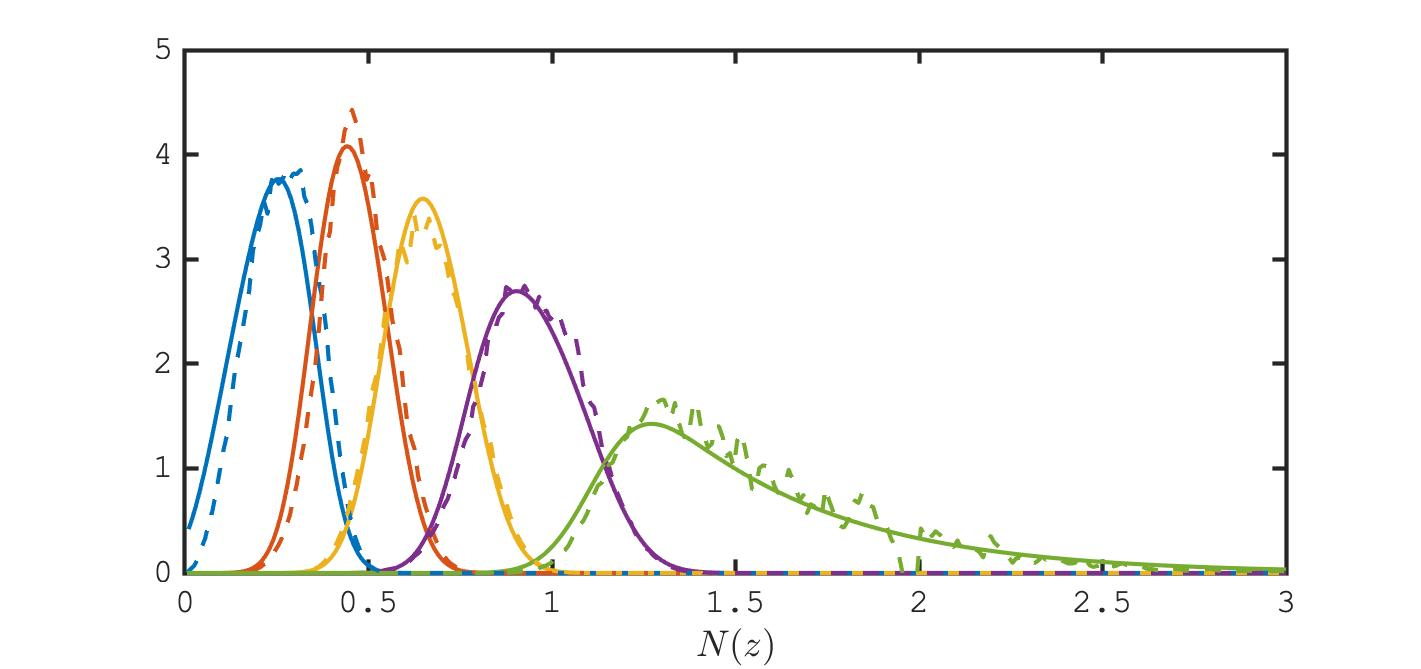
\includegraphics[width=\columnwidth]{graphs/Nz}
\caption{Redshift distributions in our simulations, either taken from the Year-1 specifications for LSST (solid) or from a matched selection applied to an HOD galaxy catalogue (dashed, see Sec. \ref{subsec:HOD}).}
\label{fig:Nz}
\end{figure}
%--------------


 Shear two-point correlation functions ($\gamma$-2PCFs hereafter) can be predicted with percent-level precision and are therefore an ideal quantity to validate weak lensing simulations. In the Limber approximation\footnote{See \citet{Kilbinger17} for a comparison between the Limber approximation and the exact calculations.}, the lensing power spectrum $C^{ij}_{\ell}$ is obtained from an integral over the three-dimensional matter power spectrum $P_{\delta}(k,z)$:
  \begin{eqnarray}
C_{\ell}^{ij} = \int_0^{\chi_{\rm H}}  \frac{q^i(\chi) \,q^j(\chi)}{\chi^2} \, P_{\delta}\, \bigg(\frac{\ell+1/2}{\chi},z(\chi)\bigg) \ {\rm d}\chi,
\label{eq:C_ell}
\end{eqnarray}
where $\chi_{\rm H}$ is the co-moving distance to the horizon, $c$ is the speed of light, $H_0$ the Hubble parameter,  and the  lensing kernels $q^{i}$ are given by:
\begin{eqnarray}
q^i(\chi) = \frac{3}{2}\Omega_{\rm m} \, \bigg(\frac{H_0}{c} \bigg)^2 \frac{\chi}{a(\chi)} \int_{\chi}^{\chi_{\rm H}} n^i(\chi')\frac{{\rm d}z}{{\rm d} \chi'}\frac{\chi' - \chi}{\chi'}{\rm d}\chi' \, .
\label{eq:q_lensing}
\end{eqnarray}
In the previous expression, $n^i(z)$ refers to the redshift distribution  in tomographic bin `$i$', while $a(\chi)$ is the scale factor at comoving distance $\chi$ from the observer.  
 The matter power spectrum is computed from  {\sc Halofit} \citep{Takahashi2012} in this work, however  other public tools provide accurate predictions, including e.g. {\sc HMcode} \citep{HMCode2020}, the {\sc EuclidEmulator} \citep{EuclidEmulator}, the {\sc Bacco} emulator \citep{BACCOEmulator} or the {\sc MiraTitan} emulator \citep{miraTitan}. 
 Predictions for the $\gamma$-2PCFs are finally computed from Eq. (\ref{eq:C_ell}) as:
 \begin{eqnarray}
\xi_{\pm}^{ij}(\vartheta) = \frac{1}{2\pi}\int_0^{\infty} C_{\ell}^{ij} \, J_{0/4}(\ell \vartheta) \, \ell \, {\rm d}\ell,
\label{eq:xipm_th}
\end{eqnarray}
where $J_{0/4}(x)$ are Bessel functions of the first kind. In this paper, these calculations are carried out by the {\sc CosmoSIS} cosmological inference package \citep{cosmoSIS}. The $n^i(z)$ are taken from the LSST Science Requirement Document \citep{LSST-SRD} and given by:
 \begin{eqnarray}
n(z) = N_0 z^2 {\rm exp} \left[-\left(\frac{z}{z_0}\right)^\alpha \right]\, ,
\label{eq:nz}
\end{eqnarray}
with $(z_0, \alpha) = (0.13, 0.78)$ and $N_0$ normalised to provide a number density of $n_{\rm eff}$ = 3.0 gal arcmin$^{-2}$. This lower than the expected number density for the first data release ($n_{\rm eff}\sim10$ gal arcmin$^{-2}$), but is large enough to validate our methods, and makes the calculation more tractable. This global $n(z)$ is further split into five equi-populated tomographic bins, and smoothed with a Gaussian filter of width $\sigma = 0.05(1+z)$ to mimic the photometric selection process [{\it confirm with Niko}], shown by the solid lines in Fig. \ref{fig:Nz}. 

The  weak lensing signal is  measured from the ellipticities $\epsilon_{1/2}$ of simulated or observed galaxies, which, in absence of systematics and secondary signals, are unbiased estimators  of the cosmic shear components $\gamma_{1/2}$. In particular, the $\gamma$-2PCF are estimated as:
 \begin{eqnarray}
 \widehat{\xi_{\pm}^{ij}}(\vartheta) = \frac{\sum_{a,b} w_a w_b \left[\epsilon_{a, \rm t}^i\epsilon_{b, \rm t}^j     \pm \epsilon_{a, \times}^i\epsilon_{b, \times}^j    \right]\Delta_{ab}(\vartheta)}{\sum_{a,b} w_a w_b} \, ,
 \label{eq:2PCF_estimator}
  \end{eqnarray}
where the sum is over all pairs of galaxies $a,b$ separated by an angular distance $\vartheta$ on the sky, respectively belonging to the tomographic bins $i$ and $j$. The tangential/cross components of their ellipticities are denoted as $\epsilon_{\rm t/\times}$, respectively. 
$\Delta_{ab}(\vartheta)$ is the binning operator, equal to unity if the angular separation between the two galaxies falls within the $\vartheta$-bin, and zero otherwise, while the shape weights $w_{a,b}$ are set to unity. In this paper, we construct lensing catalogues from numerical simulations (described in Sec. \ref{sec:sims}), from which we measure $ \widehat{\xi_{\pm}^{ij}}(\vartheta)$ with {\sc Treecorr} \citep{TreeCorr}. We set therein the {\sc bin\_slop} parameter to 0.05, then compute the correlations in 20 logarithmically-spaced angular bins with outer edges ranging from 0.5 to 475.5 arcmin. 
 
 
 %-------------------------
\subsection{Non-Gaussian lensing statistics}
\label{subsec:beyond-2pt}

Non-Gaussian statistics have the potential to extract cosmological information stored in the complex phases of the density field, outperforming in that sense the $\gamma$-2PCF that can only access information encoded in the complex amplitudes. No optimal estimator has been identified to-date as being able to capture `all' information, but numerous studies all show a clear gain in constraining power, especially when used in combination with two-point functions \citep{HD21, DESY3_Zurcher, HSC_PeaksSims}. While some of these act on galaxy catalogues directly, many non-Gaussian statistics are measured on convergence or aperture mass maps, requiring the post-process the galaxy catalogues with a mass-reconstruction algorithm. To accommodate a variety of case we therefore provide both galaxy catalogues and convergence maps, the latter being  produced from the galaxies' observed ellipticities with  the standard Kaiser \& Squires inversion technique \citep{KaiserSquires}. These are spherical {\sc Healpix}\footnote{{\sc Healpix}: http://healpix.sf.net}  maps \citep{healpix} with $N_{\rm side}=4096$ generated over an octant,  and includes a baseline 2.0 arcmin smoothing beam to suppress numerical noise. Note that this smoothing scales is quite small; some probes are difficult to model theoretically in that regime, in which case the modelling needs to be inferred from simulations directly \citep[as in][]{HD21, DESY3_Zuercher, HSCY1_Peaks_sims}. We do not discuss statistics based on aperture mass maps in this paper for the sake of conciseness, but all our methods can be applied to those estimators as well.
 
Whereas tomographic $\gamma$-2PCFs data consists of auto-correlation and cross-redshift correlations, some non-Gaussian statistics can learn additional information from analysing catalogues or maps constructed from triplets, quadruplets or quintuplet of redshift bins \citep{Martinet21a}.  We do not fully exploit this possibility here and consider auto-tomographic bin only, nevertheless all of our methods and findings can be easily generalised to include this. 
 
 
 
\subsection{Catalogue-based statistics}

A number of higher-order statistics work at the level of shear catalogue,  and here we consider the following:
\begin{enumerate}
\item {\it Three-point correlation functions (or $M_{\rm ap}^3(\vartheta)$)}:  [{\it Lucas/Laila, can you summarise the measurements and modelling, and provide references?}]
\item {\it Squeezed bispectrum}: [{\it Anik, can you summarise the measurements and modelling, and provide references?}]
\end{enumerate}

\subsection{Convergence-based statistics}

We further consider the following convergence map-based statistics:
\begin{enumerate}
\item {\it Convergence three-point correlation function}: [{\it Alejandro, can you summarise the measurements and modelling, and provide references?}]
\item {\it Peaks and Minima}: local maxima and minima in the {\sc Healpix} convergence maps are counted in bins of signal-to-noise ratios, $\nu$, computed from the global level of shape noise in the survey. These are amongst the most widely used non-Gaussian lensing statistics, as it is simple to measure yet highly sensitive to non-Gaussian structures. Although some theoretical models have been developed to describe the largest peaks \citep[see][]{Shan18, HSCY1_Peaks_th}, we report here the results on a much wider range of statistics, which can only be accurately modelled from numerical simulations.
\item {\it Lensing PDF}:  [{\it Cora/Lina, can you summarise the measurements and modelling, and provide references?}]
\item {\it Minkowski functionals}: [{\it Nisha, can you summarise the measurements and modelling, and provide references?}]
\end{enumerate}

 
 Each of these statistics probe different physical scales and non-linearities, causing their sensitivities to cosmological and systematics to vary. For example, a probe that is performing well at recovering cosmological information might be heavily affected by secondary signals such as IA and therefore deemed not robust. Having infused IA mocks at the field-level is therefore critical to answer such questions.
 
 
 %-------------------
 \section{Intrinsic alignment models}
 \label{sec:IA_th}
 %-------------------
 
Galaxies interact with the tidal forces caused by the large-scale structure  they live in, causing their intrinsic shapes to acquire correlated alignments that has nothing to do with the correlations caused by weak lensing. This therefore acts as a secondary signal that contaminates the shape correlation measurements carried out in a cosmic shear analysis. There is no consensus on the actual physical model that describes the IA signal, and even when adopting these, the free parameters they contain are only weakly constrained from the data \citep[see][for reviews]{IA_review1, IA_review2}.  %The most widely used model in the literature is the non-linear alignment model of \citet{NLA}, however it is now recognised that this is an effective model with limited precision, and the community is now progressively shifting towards more complex models. 
In this paper we consider two coupling models each applied on three galaxy bias cases, resulting in six different IA models, described in the following sub-sections. In all cases, our models couple the galaxy intrinsic shapes with the local over-density and projected tidal field, then prescribes an intrinsic ellipticity tensor $\gamma_{ij}^{\rm IA}$, from which intrinsic  ellipticities are extracted:
 \begin{eqnarray}
\epsilon_{1}^{\rm IA} = \gamma_{xx}^{\rm IA} - \gamma_{yy}^{\rm IA} \, , \hspace{1.5cm}\epsilon_{2}^{\rm IA} = 2 \gamma_{xy}^{\rm IA}\, .
\label{eq:tidal_th_deltaNLA}
\end{eqnarray}


 
\subsection{Non-linear alignment (NLA)}

 
%The observed ellipticity of a galaxy ${\boldsymbol \epsilon}_{\rm obs} $ is a combination of its intrinsic shape ${\boldsymbol \epsilon}_{\rm int}$ and a cosmic shear signal ${\boldsymbol \gamma}$, the former of which can be further divided in a random component ${\boldsymbol \epsilon}^{\rm ran}$ and an alignment term ${\boldsymbol \epsilon}^{\rm IA}$.
The NLA model of \citet{NLA} is the most widely used IA model in the cosmic shear literature thus far. According to the NLA, IA are caused by a linear coupling between galaxy shapes and the non-linear large-scale tidal field at the galaxy position. The intrinsic ellipticities $\epsilon_{1,2}^{\rm NLA}$ are related to tidal field $s_{ij}$ by:
 \begin{eqnarray}
\epsilon_1^{\rm NLA} = - \frac{A_{\rm IA}\bar{C_1}\bar{\rho}(z)}{D(z)} (s_{xx} - s_{yy}) \,\,\,\,,   \epsilon_2^{\rm NLA} = - \frac{2 A_{\rm IA}\bar{C_1}\bar{\rho}(z)}{D(z)} s_{xy}\;,
\label{eq:tidal_th}
\end{eqnarray}
where $s_{ij} = \partial_{ij}\phi$ are the Cartesian components of the tidal tensor of the gravitational potential,  $D(z)$ is the linear growth factor, $\bar{\rho}(z)$ is the mean matter density at redshift $z$ and $\bar{C_1}=5\times 10^{-14} M_{\odot}^{-1} h^{-2} {\rm Mpc}^3$ is a constant calibrated in \citet{Brown2002}. The strength of the tidal coupling is modulated by the amplitude parameter $A_{\rm IA}$, which is the main NLA parameter constrained by current cosmic shear surveys. Note that this model can be augmented by redshift and luminosity dependences, however we do not use these here. Also note that the term `non-linear' in the model name can be  misleading, as it refers to the non-linear matter power spectrum $P(k)$ that is used in its calculations; the coupling between the intrinsic galaxy shapes and the tidal field is still linear and   Eq.( \ref{eq:tidal_th}) is used to assign intrinsic ellipticities to galaxies, given maps of the tidal field components $s_{xx}$, $s_{yy}$ and $s_{xy}$ (presented in  Sec. \ref {subsec:IA_infusion}).





In the context of  two-point functions, these intrinsic shapes contribute to an intrinsic-intrinsic ($II$) term and an intrinsic-shear coupling ($GI$) term \citep{Hirata2004}, both secondary signals to the true cosmic shear ($GG$) term, with the $GI$ typically dominating the IA sector in cross-tomographic measurements.  The $II$ and $GI$ terms  can be both computed from the matter power spectrum as: 
 \begin{eqnarray}
P_{II}(k,z) =  \left(\frac{A_{\rm IA}\bar{C_1}\bar{\rho}(z)}{D(z)}\right)^2a^4(z) P_{\delta}(k,z)
\label{eq:Pk_II_th}
\end{eqnarray}
and
 \begin{eqnarray}
P_{GI}(k,z) = - \frac{A_{\rm IA}\bar{C_1}\bar{\rho}(z)}{D(z)}a^2(z) P_{\delta}(k,z) \, ,
\label{eq:Pk_GI_th}
\end{eqnarray}
which can then be past to the Limber integration (Eqs. \ref{eq:C_ell} and \ref{eq:xipm_th}) to compute  the secondary signals $\xi_{\pm}^{II}(\vartheta)$ and $\xi_{\pm}^{GI}(\vartheta)$. 


\subsection{$\delta$-NLA}
\label{subsec:IA_th_ext}

%[{\it here}]

%As discussed later, the key quantity of interest to cosmic shear analysis is not the tidal tensor itself but its trace-free version, since shape correlations with the density field are subdominant, even though peaks in high density environments are less elliptical on average. Consequently, the model itself has a restricted range of validity: on small scales, higher order couplings to the ellipticity field ${\boldsymbol \epsilon}^{\rm IA}$  become important, however these are neglected in the NLA model. Only the non-linear evolution of the tidal tensor itself is taken into account, since it does fit observations quite well.

%We note that the NLA predicts additional higher-order terms and non-zero $B$-modes \citep{Hirata2004} that we neglect  in this analysis. Also, as shown in \citet{IA_EFT}, the NLA model can be interpreted as the lowest order description of the alignment process of galaxies in the light of an effective field theory description. 


The NLA model presented in the last section has been widely used in cosmic data analyses, but it has important known limitations and is therefore bound to fail at describing the IA signal with high precision.
A perturbation theory extension to the NLA has been introduced in \citet{Blazek2015} and  \citet{Blazek2019},  where it is recognised that higher order couplings could be important and should be considered. The first additional term to be included is an over-density weighting term, which arises from the fact that  the intrinsic alignment of galaxies can only be observed at the galaxy positions, which are not distributed randomly on the sky but instead trace the underlying matter density.  Accounting for this extra term in theoretical predictions is done with one-loop perturbation theory  \citep{Blazek2019} by assuming that the over-density  `$\delta$' is linearly traced by the galaxies. Physically, it corresponds to adding a $\delta$-weight to the NLA predictions at the local galaxy positions. At the level of numerical simulations, this could be done in principle simply by augmenting the NLA ellipticities with this weight, namely:
 \begin{eqnarray}
\epsilon_{1/2}^{\delta-\rm NLA} = \epsilon_{1/2}^{\rm NLA}\times(1 + b_{\rm TA}\delta) \, ,
\label{eq:tidal_th_deltaNLA}
\end{eqnarray}
where the term $b_{\rm TA}$ corresponds to the (largely unconstrained) biasing relation between the galaxies and the underlying matter field. In practice however, we find this method to be noisy, as many galaxies placed at random actually live in regions of negative or small $\delta$. It is instead preferable to generate mock catalogues with the linear biasing directly applied when assigning galaxy positions, after which no weighting is necessary. Subsequently, Eq. (\ref{eq:tidal_th_deltaNLA}) can be used to modify the value of the effective $b_{\rm TA}$ if not wanting to re-populate the light-cone. Indeed, from a mock with a given bias $b_{\rm TA, orig}$, we can rescale the IA contribution to a different $b_{\rm TA, new}$  as:
\begin{eqnarray}
{\boldsymbol \epsilon}^{\rm int}_{b_{\rm TA, new}}  = \frac{(1 + b_{\rm TA, new}\delta)}{(1 + b_{\rm TA, orig}\delta)}{\boldsymbol \epsilon}^{\rm int}_{b_{\rm TA, orig}} \, .
\label{eq:bta_rescale}
\end{eqnarray}


Compared to the NLA, the $\delta$-NLA is a stronger IA model, especially on small scales \citep{Blazek2019}, and seems to be preferred by some hydrodynamical simulations \citep{Hilbert_IA2017}. It is also better motivated from a physical point of view, since galaxies are not randomly distributed in our Universe as the NLA assumes. 

Finally, we note that fully modelling our infusion method includes contributions beyond one-loop calculations in the $II$ term. Indeed, the two-point function correlating ellipticities (Eq. \ref{eq:tidal_th_deltaNLA}) between redshift bins $i,j$ is given by:
 \begin{eqnarray}
\langle \epsilon_{i}^{\delta-\rm NLA} \epsilon_{j}^{\delta-\rm NLA}\rangle &=& \langle \epsilon_{i}^{\rm NLA}\times(1 + b_{\rm TA}\delta_i) \epsilon_{j}^{\rm NLA}\times(1 + b_{\rm TA}\delta_j)\rangle\\
&=& \langle \epsilon_{i}^{\rm NLA}  \epsilon_{j}^{\rm NLA}\rangle \nonumber \\
&+& b_{\rm TA} \times \left(\langle \epsilon_{i}^{\rm NLA}  \epsilon_{j}^{\rm NLA}\delta_j  \rangle + \langle \epsilon_{i}^{\rm NLA}  \epsilon_{j}^{\rm NLA}\delta_i  \rangle \right)\nonumber\\
&+& b_{\rm TA}^2 \langle \epsilon_{i}^{\rm NLA}  \epsilon_{j}^{\rm NLA}\delta_i  \delta_j \rangle \, ,
\label{eq:2pcf_deltaNLA}
\end{eqnarray}
where the last term is fourth order and involves two-loop calculations. For this reason, our $\delta$-NLA model is not expected to be well described by the one-loop calculations. Note that replacing one of the ellipticity terms by the cosmic term includes only terms up to third order in the field (e.g $\langle \epsilon_{i}^{NLA}\delta_i \gamma_j \rangle$, ...), hence  we expect the GI term to be well described. The above equation also predict that the deviations from one-loop theory scales as $b_{\rm TA}^2$, hence should be larger for population that are more biased.

%-----------------------------------
\subsection{Tidal Torque (TT)}
\label{subsec:IA_th_TT}

As shown in \citet{Blazek2019}, one-loop perturbative calculations include another term, by which galaxies acquire an intrinsic alignment via a coupling between their angular momentum and the tidal field, which can be re-expressed as a quadratic coupling between the tidal field and their shape. In this tidal torque model (TT), intrinsic ellipticities are given by:
\begin{eqnarray}
\gamma_{ij}^{\rm IA, TT} = C_2 \left[ \sum_{k=x,y,z} s_{ik} s_{kj} -\frac{1}{3} \delta_{ij} s^2 \right] \, ,
\label{eq:tidal_th_TT}
\end{eqnarray}
where 
\begin{eqnarray}
C_2 = \frac{5 A_2 \bar{C_1} \Omega_{\rm m} \rho_{\rm crit}}{D^2(z)} \,  = \left[ \frac{-5 A_2}{A_1 D(z)} \right] C_1.
\end{eqnarray}
Under the approximation that line-of-sight alignments are mostly suppressed from cosmic shear measurement due to the broad lensing kernels, 
we show in  Appendix \ref{app:2d_TT} that the terms inside the square bracket in Eq. (\ref{eq:tidal_th_TT}) leads to:
\begin{eqnarray}
\epsilon_1^{\rm TT} = C_2  \left[ s_{xx}^2 - s_{yy}^2\right] \, , \epsilon_2^{\rm TT} = 2 C_2 s_{xy}\left[s_{xx}+s_{yy}  \right]\, ,
\end{eqnarray}
both quadratic in the tidal field components. In this model, galaxies are also assumed to be randomly distributed on the sky; the $\delta$-weighted term requires third order perturbations.


%-----------------------------------
\subsection{$\delta$-TT}
\label{subsec:IA_th_TT}

%Following the relation between the NLA and the $\delta$-NLA model, galaxies in the TT model are also assume to be randomly scattered on the sky, which we know to be a bad approximation. 
Computing the next-order contribution to the TT model involves two-loop perturbation theory calculations that have not been carried out  yet due to the significantly complexity of such task. In simulations however, the $\delta$-weighting term is straight-forward to implement, as it involves to simply infuse the TT model onto galaxies that trace the matter field with a non-zero biasing factor. As for the $\delta$-NLA model, the $\delta$-TT ellipticities can  be related to the TT model as:
\begin{eqnarray}
\epsilon_{1/2}^{\delta-\rm TT} = \epsilon_{1/2}^{\rm TT}\times(1 + b_{\rm TA}\delta) \, ,
\label{eq:tidal_th_deltaTT}
\end{eqnarray}
however we choose instead here again to use galaxy positions that themselves are linearly biased.
As there are currently no theoretical models for $\delta$-TT, predictions from this model are, at the moment, completely simulation-based. 
 
 %-----------------------------------
\subsection{$b_{\rm nl}$-TATT}
\label{subsec:HOD-TATT}

The previous four models combine the linear and quadratic couplings to the cosmic tidal forces  (Eqs. \ref{eq:tidal_th} and \ref{eq:tidal_th_TT} respectively) with galaxies positioned  either at random or linearly tracing the total matter distribution. While these are interesting and useful approximations, the connection between galaxies and dark matter is far more complex, and a more accurate picture consists of galaxies populating dark matter haloes, typically with a relaxed, older galaxy close to the centre, and a number of other satellite galaxies orbiting the former. This halo occupation distribution (HOD) formalism has been used to describe many galaxy samples \citep[e.g.][]{SDSS-HOD, BOSS-HOD, GAMA-HOD, DESI-HOD} and is therefore routinely used to in-paint galaxies in dark matter-only simulations. The last two models from this paper exploit such HOD galaxy samples, extracted from the same underlying distributions, but in this case the galaxy bias is non-linear (labelled $b_{\rm nl}$), with levels on non-linearity that vary with HOD parameters (see Sec. \ref{subsec:HOD}).  We couple these galaxies with both Eqs. \ref{eq:tidal_th} and \ref{eq:tidal_th_TT}, resulting in two final models which we name  $b_{\rm nl}$-NLA and  $b_{\rm nl}$-TT, both being combined into the more general  $b_{\rm nl}$-TATT model.


%Finally, it is worth recalling here that other IA models exist in the literature, and that at this point observations are not precise enough to set strong constraints on them, further motivating our flexible multi-model approach.  


%\subsection{Likelihood}
%\label{subsec:likelihood}

%Multi-Gaussian likelihood, analytical Covariance matrix (Gauss + non-Gauss + SSC) from {\sc TJPCov}, Firecrown, sampler, priors.

%---------------------
\section{Simulations}
\label{sec:sims}

%-------------
\subsection{Cosmic shear galaxy catalogues} 
\label{subsec:WL_cats}

The weak lensing simulations developed for this work are based on ray-tracing mass sheets produced from the {\it Outer Rim} $N$-body simulation \citep{OuterRim}, which evolved 10,240$^3$ particles in a (5.225 Gpc)$^3$ cosmological volume, assuming a flat $\Lambda$CDM cosmology with $\Omega_{\rm m}$=0.2648, $\Omega_{\rm b}$=0.0448, $h$=0.71, $\sigma_8$ = 0.801, $n_{\rm s}$= 0.963, $w_0$=-1.00. A total of 101 particle snapshots were originally saved, of which we use only those with $z<4.0$. Particles from each dump are assigned to curved mass shells approximately 114 Mpc thick, producing a sequence of 57 {\sc Healpix} maps $\delta(\theta,\phi,\chi_i)$ with {\sc nside} = 8192 and $i=1..57$, filling up a light-cone over an octant up to $z=3$. %More details on this procedure can be found  in \citet{cosmoDC}, where lensing quantities are computed specifically for the generation of the {\sc cosmoDC2}  synthetic sky catalogue.

Ray-tracing is performed in the Born approximation, summing over the mass shells using the $\chi$-integral of Eq. (\ref{eq:C_ell}). A source plane is placed at the high-redshift edge of every mass planes, resulting in a series of convergence  maps  $\kappa(\theta,\phi,\chi_i)$ that are subsequently transformed into shear maps $\gamma_{1/2}(\theta,\phi,\chi_i)$ using the Kaiser-Squires methods \citep{KaiserSquires}, which is implemented via efficient {\sc HealPy alm2map} routines. We finally position galaxies in the light cone following three distinct algorithm, each impacting the strength of the IA signal:
\begin{enumerate}
\item {\it Random:} galaxies are distributed randomly on the octant, thereby reproducing one of the  fundamental assumptions in the NLA and TT models. 
\item {\it Linear bias:} galaxy positons are sampled from the mass sheets smoothed\footnote{We also tried sampling the field with 0.1 and 0.5 $h^{-1}$Mpc but this resulted in noisier results.} with a  1.0 $h^{-1}$Mpc (comoving) beam, assuming a linear bias of $b_{\rm TA}$, thereby building the one of the key assumptions of the $\delta$-NLA and $\delta$-TT models. We assume $b_{\rm TA}=1.0$ as our fiducial case but also consider $b_{\rm TA}=2.0$ to test  the  model flexibility. 
\item{\it Non-linear bias:} galaxy positions are obtained by populating dark matter haloes with the Halo Occupation Distribution prescription described in \citet{cosmoDC2}. 
\end{enumerate}
Note that while cases (i) and (ii) exactly the SRD-Y1 $N(z)$ presented in Fig. \ref{fig:Nz} (solid lines), the $N(z)$ in the latter case is not a perfect match (dashed lines); we return to this in Sec. \ref{subsec:HOD}, where we describe the HOD model and related quantities.  


%----------
\subsection{Projected tidal fields}
\label{subsec:IA_sims}

\begin{figure*}
\caption{Density field and the associated projected tidal field tensors.}
\label{fig:maps}
\end{figure*}

Our infusion method completely relies on couplings between intrinsic galaxy shapes and the local tidal field, hence the first step in our method consist in extracting the tidal field maps $s_{ij}(\theta,\phi,\chi_i)$ from the mass maps $\delta(\theta,\phi,\chi_i)$ that source them. In three dimensions, trace-free tidal tensor $s_{ij}(\boldsymbol x)$ can be obtained from the matter over-density field $\delta(\boldsymbol x)$ as   \citep{Catelan_IA_Tidal}:
\begin{eqnarray}
 \widetilde{s}_{ij} (\boldsymbol k)  = \left[\frac{k_i k_j}{k^2} - \frac{\delta_{ij}}{3}\right]  \widetilde {\delta}(\boldsymbol k) \mathcal{G}(\sigma_{\rm G}) \, ,
 \label{eq:sij}
\end{eqnarray}
where $\mathcal{G}(\sigma_{\rm G})$ is a three-dimensional Gaussian function described by a single (free) parameter $\sigma_{\rm G}$ that  controls the physical scales which are allowed to affect the IA term in our model. 
Tilde symbols  denote Fourier transformed quantities,  the indices $(i,j)$ label the components of the Cartesian wave-vector $\boldsymbol{k}^T = (k_x,k_y,k_z)$, and $k^2 = k_x^2 + k_y^2 + k_z^2$. 
As shown in \citet{Tidalator} for Cartesian coordinates, projected tidal fields  computed from projected mass sheets provide and excellent agreement with the NLA model, which in contrast computes the full tidal fields from the three-dimensional matter density and project along the radial dimension at the end. We promote this transformation to curved-sky in this work, exploiting the  polarisation {\sc alm2map} operations built in {\sc Healpy}. In particular, noting that $Q=s_{xx}-s_{yy}$, $U=s_{xy}$ and $\delta=s_{xx}+s_{yy}$, we compute the curved-sky tidal field tensors ${s}_{ij}({\boldsymbol \theta})$ as:
 \begin{eqnarray}
s_{xx}({\boldsymbol \theta})  =  \left[\frac{ \delta + Q}{2}  - \frac{\delta}{3}\right] \, ,s_{yy}({\boldsymbol \theta})  =  \left[\frac{\delta - Q}{2}  - \frac{\delta}{3}\right] \, , s_{xy}({\boldsymbol \theta}) = U
 \label{eq:sij_2D_sph}
 \end{eqnarray}
where the $U({\boldsymbol \theta})$ and $Q({\boldsymbol \theta})$ maps are smoothed by the Gaussian beam with width $\sigma_{\rm G}$. We suppress large artificial tidal fields at the maps boundary by replicating 8$\times$ the density maps defined on the octant and working on a full sky density $\delta$; we re-apply the octant mask on the tidal field maps after the operation. Note that the value of $\sigma_{\rm G}$ is a free parameter both in the infusion technique described in this paper and in the NLA and TATT models. We therefore explore two cases, $\sigma_{\rm G}=0.1$Mpc and 0.5Mpc, however this may be further optimised in the future. Finally, the full-sky density field is downgraded from $N_{\rm side}=8192$ to $N_{\rm side}=4096$ since the smoothing washed the smallest angular scales. 



%are specified within the NLA model. Smoothing amounts to selecting physical scales that do not contribute to the alignment of galaxies, which is still a debatable quantity, but is also introduced for numerical stability. \citet{Blazek2015} argues that 1.0 $h^{-1}$Mpc could be a reasonable fiducial value, being larger then the typical halo size, but recognizes that one-halo terms are also required to better match the observations. In their later work, \citet{Blazek2019} do not include smoothing at all, and neither do the KiDS-1000 nor DES-Y1 analyses based on the NLA model \citep{KiDS1000_Asgari,DESY1_Troxel}. In this work we used a two-dimensional Gaussian filter and calibrated $\sigma_{\rm G}$ empirically to $\sigma_{\rm G}=0.1h^{-1}$Mpc (see Sec. \ref{subsubsec:sigma_G}), however these two choices are arbitrary and could possibly be better optimised in the future; we also explore $\sigma_{\rm G}=0.5h^{-1}$Mpc later on.  We note that the smoothing scale is degenerate with the resolution of the simulation itself, and that one should use caution when smoothing on scales that approach the resolution limits.

%We employ a numerical technique worth mentioning here: the Fourier transforms involved in computing Eq. (\ref{eq:sij_2D}) are computed from the full (projected) periodic boxes of the simulations, then interpolated on the light-cones. We find that tidal field computed directly from the $10\times10$ deg$^2$ light-cones introduces significant large scales features in the tidal field maps, largely caused by  the non-periodic boundary conditions, which our method avoids.
Projected tidal field maps $s_{11}$, $s_{22}$ and $s_{12}$ are constructed that way for each mass sheets; Fig. \ref{fig:maps} shows the  three tidal fields and the mass maps for one of them. We can clearly see the connection between all maps around over-dense regions. {\it (Include a figure of $s_ij$ and $\delta$)}. 

{\it [Mention normalisation of the tidal fields by $0.6252 = H_0/114$ = 1/shell-thickness}

%of every light-cones and interpolated at the position of every galaxy. Fig. \ref{fig:tidalator} illustrates this process for a small zoomed-in patch at $z\sim0$, starting from a $\delta_{2D}(\boldsymbol \theta)$ map (upper large panel), computing the tidal field components (middle four panels) and comparing the results with the cosmic shear signal generated by the same mass distribution (bottom two panels). The tidal field maps clearly reproduce the cosmic shear maps, and the minus sign in front of both terms in Eq. (\ref{eq:tidal_th}) causes the IA to undo some of the lensing signal.

\subsection{Infusion of intrinsic alignments}
\label{subsec:IA_infusion}

Having now produced shear catalogues and tidal field maps, we can now use Eq. \ref{eq:tidal_th} to couple linearly the alignment of galaxies with the local tidal field, or Eq. \ref{eq:tidal_th_TT} to use instead a quadratic coupling. These allow us to compute the intrinsic ellipticities ${\boldsymbol \epsilon}^{\rm int}$ for the four IA models described in Sec. \ref{sec:IA_th}, which we combine with the cosmic shear signal ${\boldsymbol g}$ to compute observed ellipticities: 
\begin{eqnarray}
{\boldsymbol \epsilon}^{\rm obs} = \frac{{\boldsymbol \epsilon}^{\rm int} + {\boldsymbol g}}{1 + {\boldsymbol \epsilon}^{\rm int}{\boldsymbol g^*}} \,, {\rm with \, \, } 
{\boldsymbol \epsilon}^{\rm int}  = \frac{{\boldsymbol \epsilon}^{\rm IA} + {\boldsymbol \epsilon}^{\rm ran}}{1 + {\boldsymbol \epsilon}^{\rm IA}{\boldsymbol \epsilon^{\rm ran, *}}}.
\label{eq:eps_obs}
\end{eqnarray}
In the above expressions, the denominators ensures that the combined  ellipticities never exceed unity.
The complex spin-2 reduced shear ${\boldsymbol g} \equiv (\gamma_1 + {\rm i} \gamma_2)/(1+\kappa)$ is computed from the shear  $(\gamma_{1/2}$) and convergence ($\kappa$) maps, interpolated at the galaxy positions and redshifts. The  random orientation term ${\boldsymbol \epsilon}^{\rm ran}$ is drawn from two Gaussians (one per component) with their standard deviations matching the LSST-Y1 forecast, $\sigma_{\epsilon} = 027$. We further constraint  the random ellipticity to satisfy $|{\boldsymbol \epsilon}^{\rm ran}| \le 1.0$. 
%We recall that since our simulated galaxy catalogues trace the dark matter density, our default IA-infusion method  is consistent with the $\delta$-NLA model (see Sec. \ref{subsec:IA_th_ext}). Analytical predictions for the two-point functions are more involved in this case \citep[see][]{Blazek2019} and not yet available on the public {\sc cosmoSIS} release. We therefore validate our methods with the standard NLA first, which we infuse by `correcting' the $\delta$-NLA measurement with Eq. (\ref{eq:tidal_th_deltaNLA}), i.e. by replacing ${\boldsymbol \epsilon}^{\rm IA}$ by ${\boldsymbol \epsilon}^{\rm IA}/(1 + b_{\rm TA} \delta)$ in our simulations. Once again, these are less realistic but better suited for validation of the measured $\gamma$-2PCFs against a theoretical model; after this is established, we use the $\delta-$NLA catalogues as our fiducial infusion model. 
We re-iterate here that the same tidal fields, shear maps and IA coupling equations are used for the NLA and $\delta$-NLA models, and separately for the TT and $\delta$-TT models; these  only differ by the fact that in one case the galaxies are placed at random on the octant, while in the other case they are linearly tracing the dark matter.


Also note that our current IA models make no differentiation between galaxy colours or type, and instead treats the full sample as a single population that has a single, effective, alignment signall \citep[see][for an example with a red/blue split]{DESY1_IA_Samuroff}.


Finally, once all galaxies have been placed in the light-cone, we interpolate the shear and IA quantities at their exact location.

%---------------------
\section{Validation with $\xi_{\pm}$}
\label{sec:validation}




% Requires the booktabs if the memoir class is not being used
\begin{table}
   \centering
   %\topcaption{Table captions are better up top} % requires the topcapt package
   \begin{tabular}{@{} lcr @{}} % Column formatting, @{} suppresses leading/trailing space
      \hline
      \hline
       %\multicolumn{2}{c}{Item} \\
      model   		& ($A_{\rm IA}, b_{\rm TA}, A_2)$ \\
      \hline
      NLA     		& {($\pm$1,0,0) }&  \\
      \multirow{2}{*}{$\delta-$NLA }  	&   {($\pm$1,1,0)}   \\
      							&  {(1,2,0)}   \\
      TT 			&  {(0,0,$\pm$1)} &  \\
      \multirow{2}{*}{$\delta$-TT} 	&  {(0,1,$\pm$1)}   \\
      				&  {(0,2,1)}   \\
      TATT- fiducial	&  { (1,1,1)}  \\
      %TATT-DESY3	&   (-0.7,1,1.9) & \\
      \hline
      \hline

   \end{tabular}
   \caption{IA models infused in this work.}
   \label{table:IAmodels}
\end{table}


%------------------------------
\subsection{NLA model}
\label{subsubsec:sigma_G}

See Fig. \ref{fig:xi_NLA}
%---------------
\begin{figure*}
%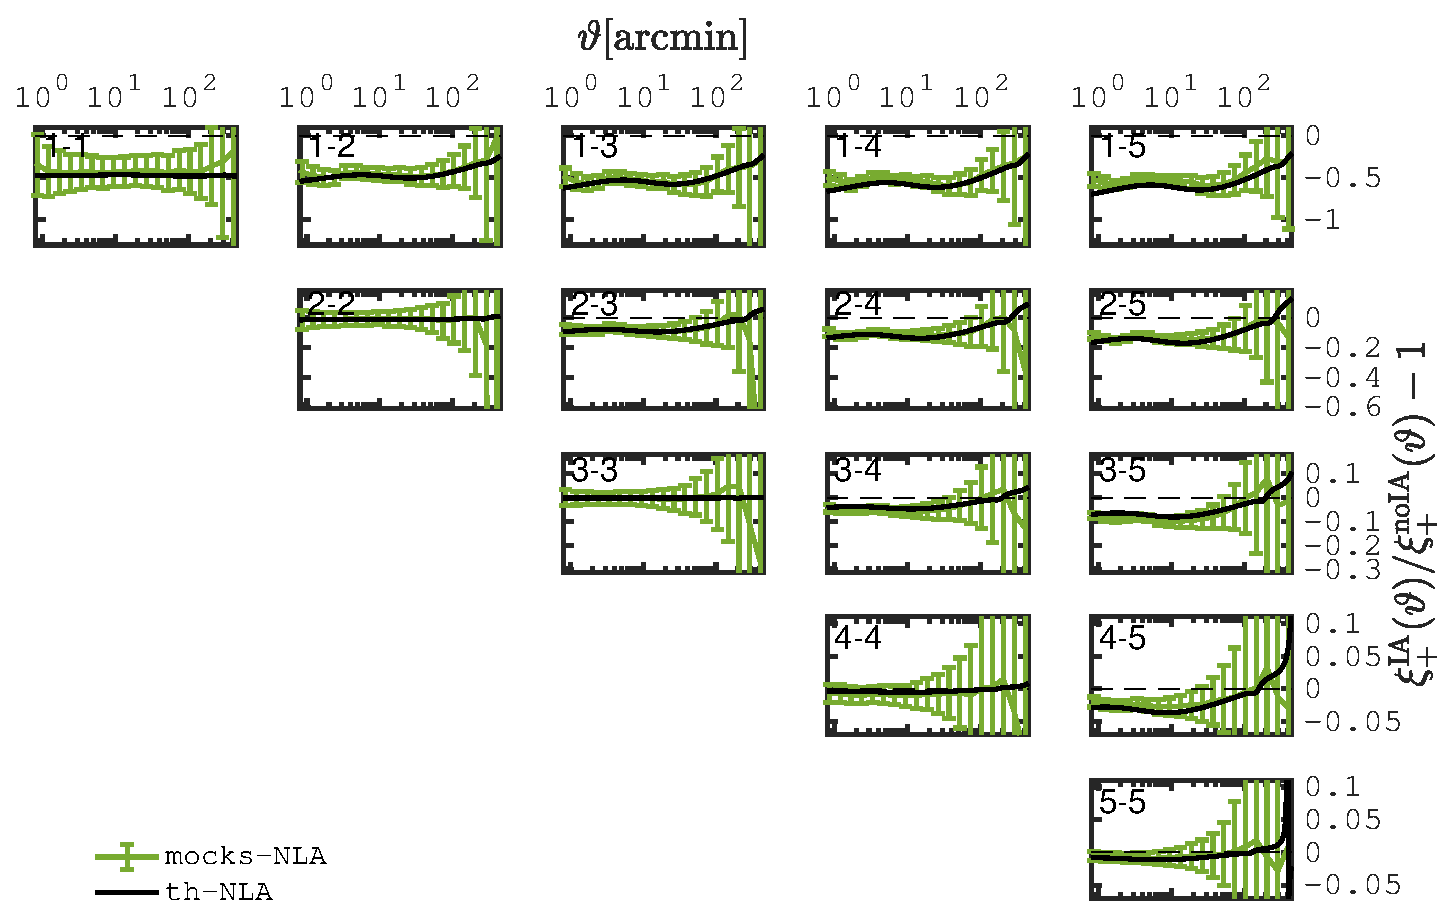
\includegraphics[width=\columnwidth]{graphs/frac_xip_IA1_skysim}
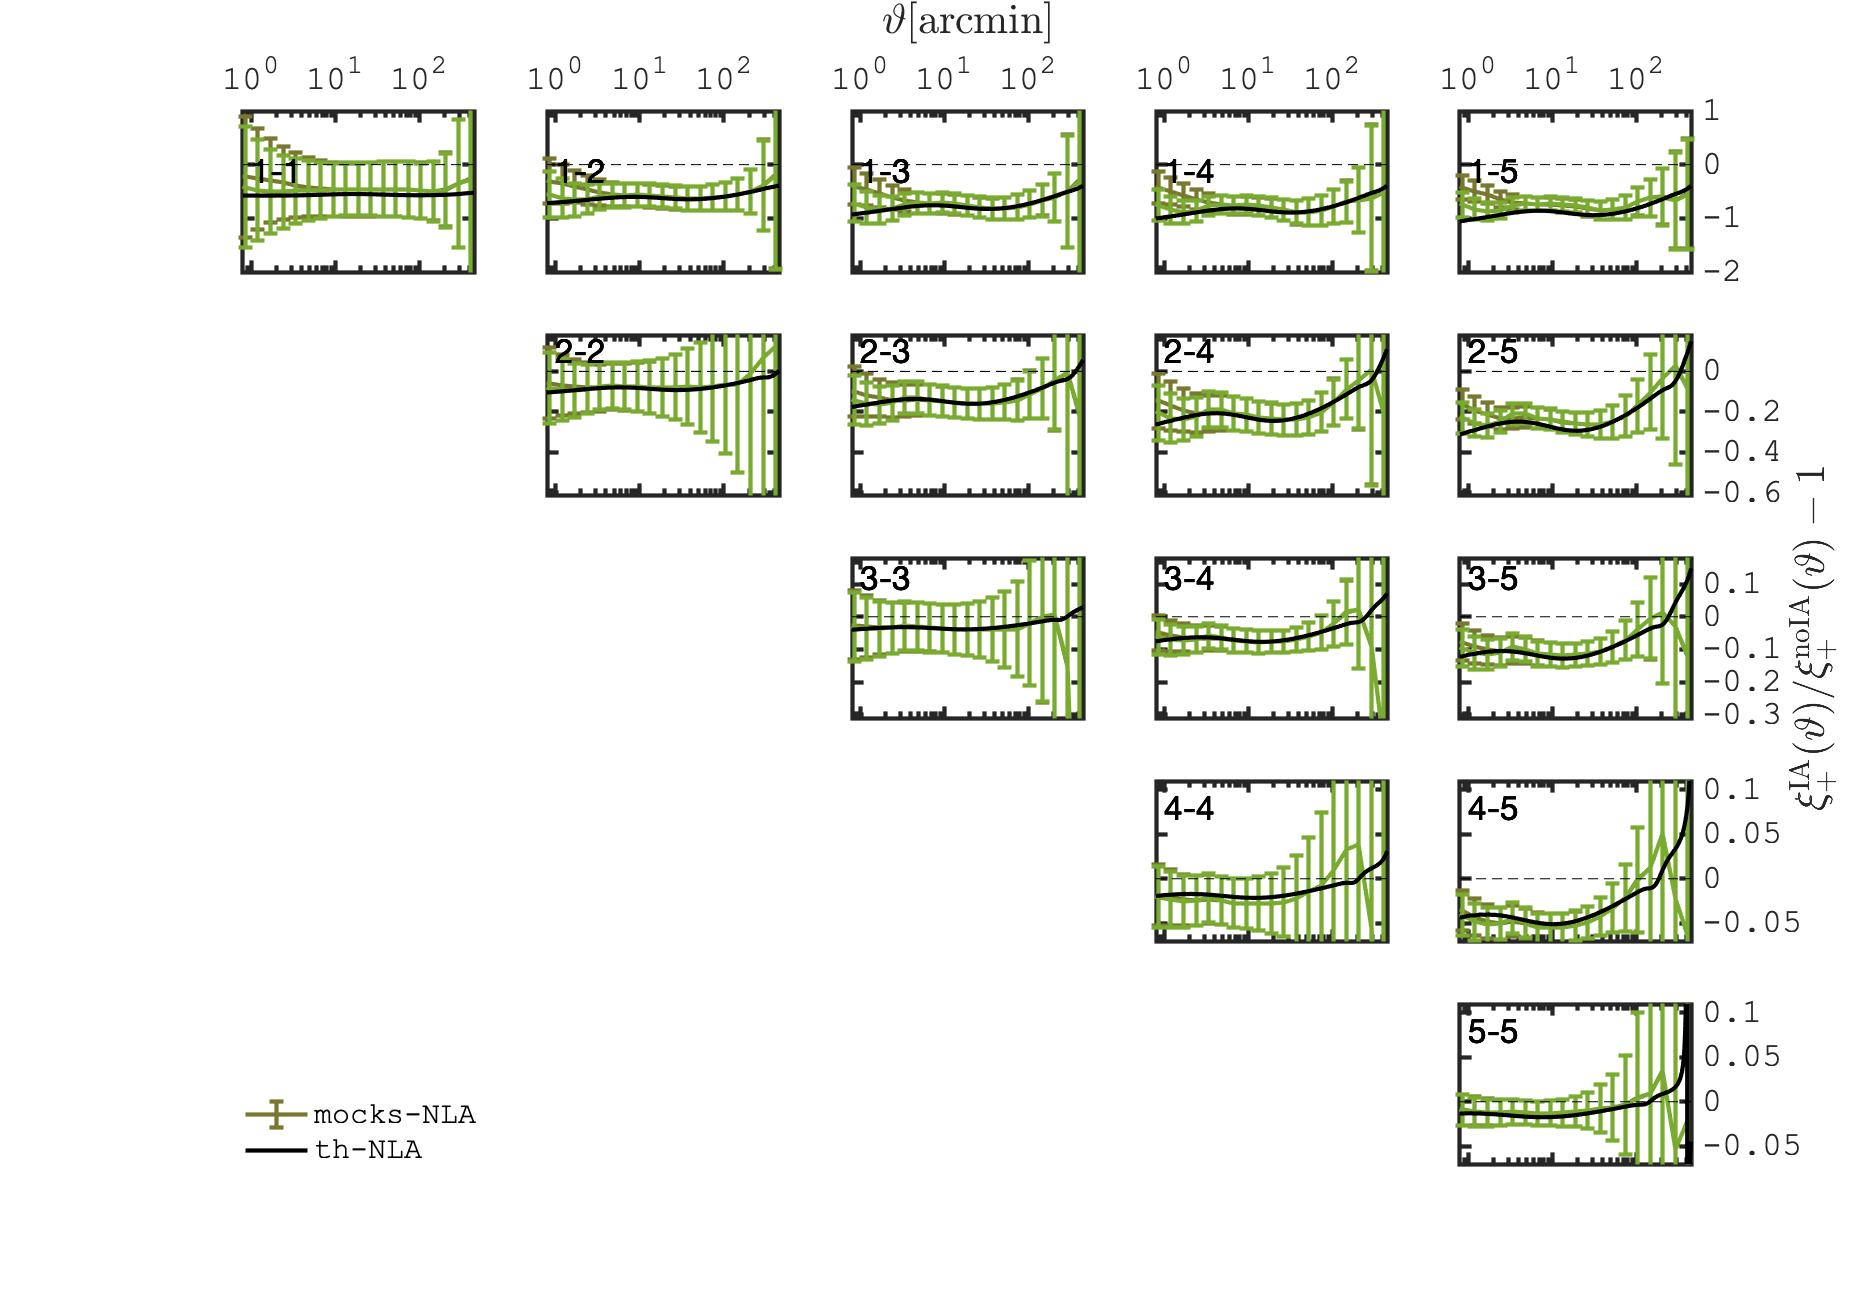
\includegraphics[width=\columnwidth]{graphs/frac_xip_IA1_skysim_NLA_srd.jpg}
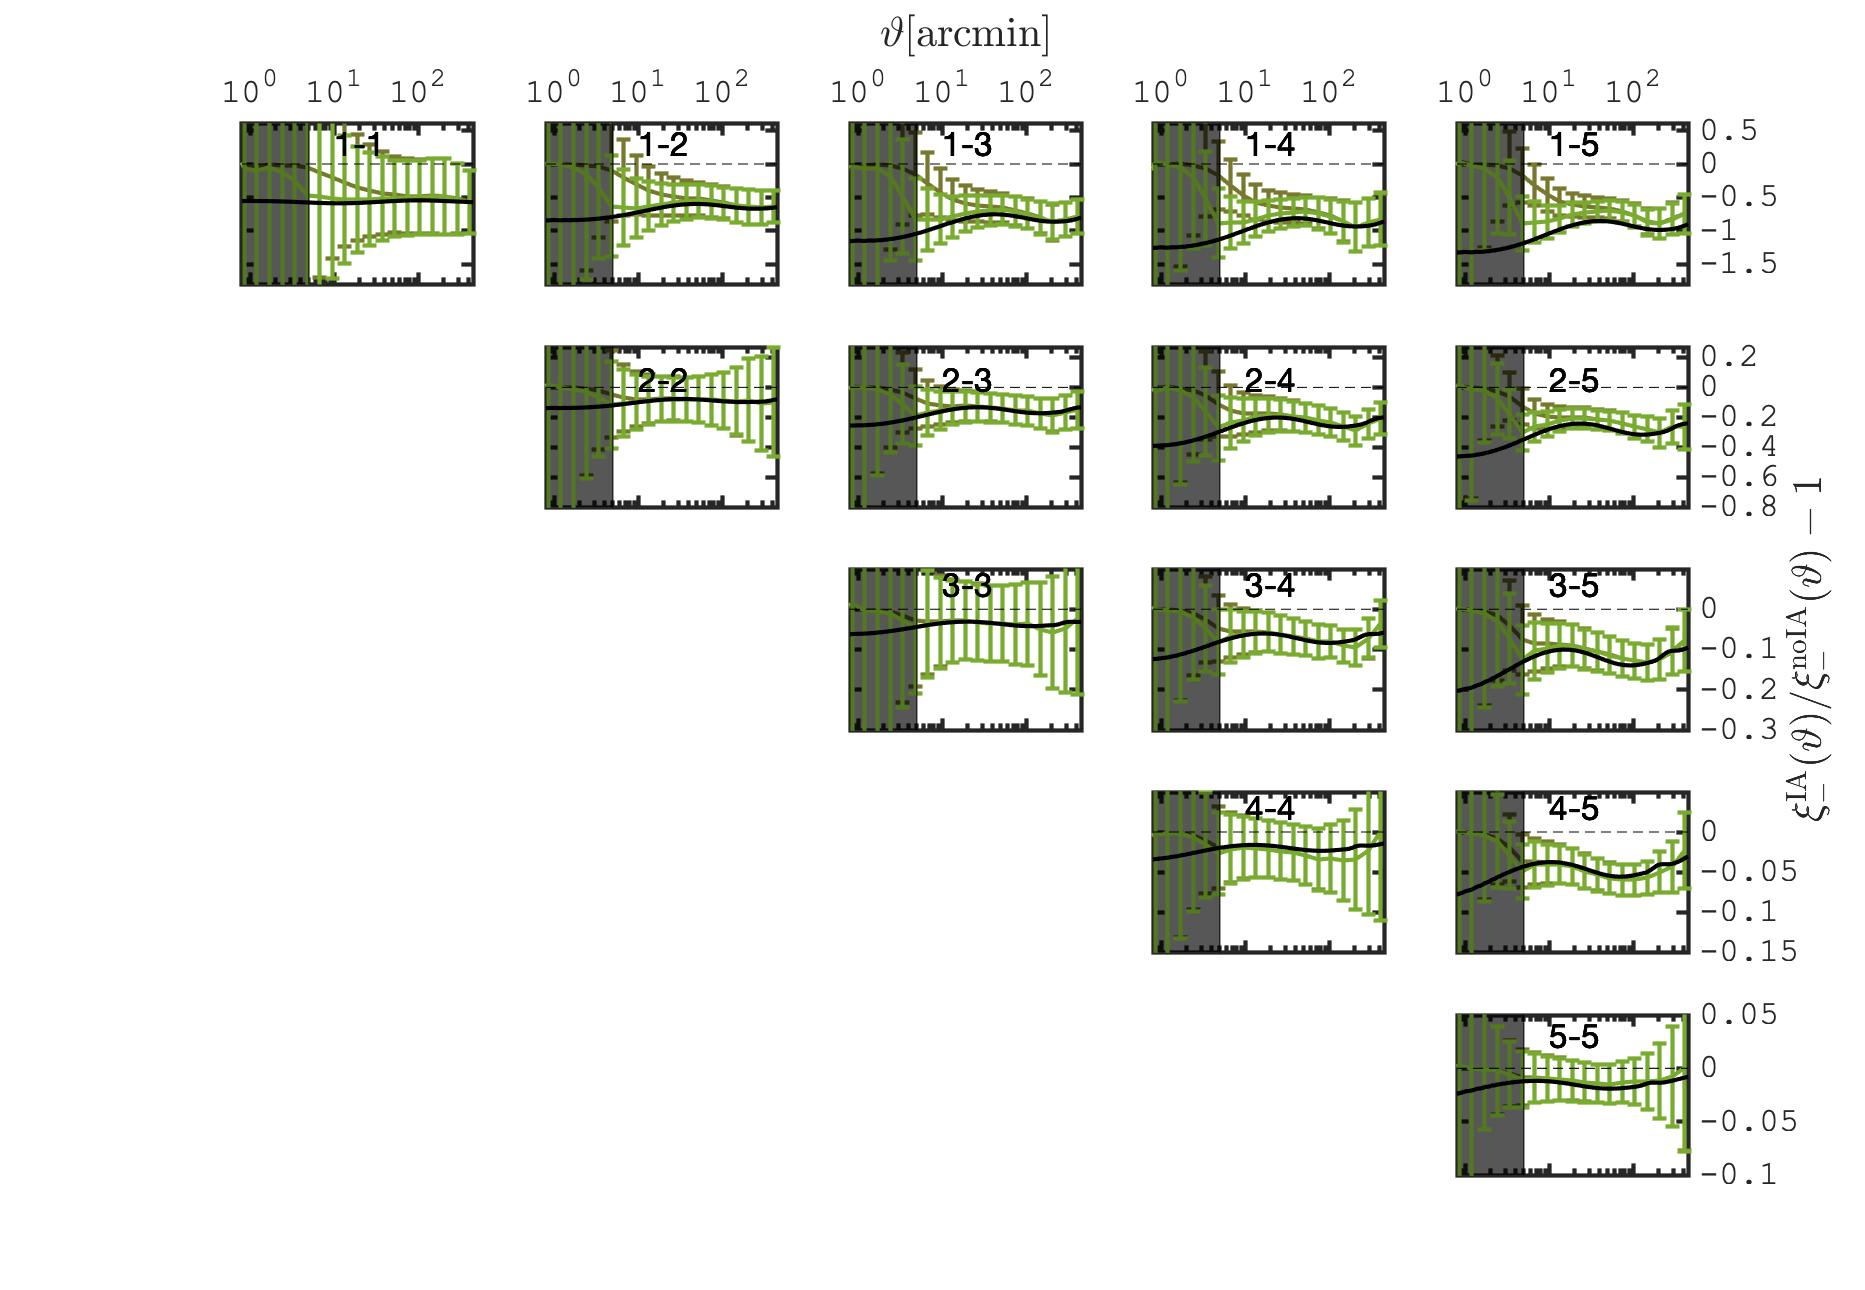
\includegraphics[width=\columnwidth]{graphs/frac_xim_IA1_skysim_NLA_srd.jpg}
\caption{Ratio between the shear correlation functions with and without IA, assuming the NLA model with $A_{\rm IA}=1.0$ both in the simulations and theory. Measurements shown in green and brown correspond to smoothing scales of 0.1 and 0.5 $h^{-1}$Mpc in the tidal field. There is no shape noise in the simulations, but it is included in the error bars.}
\label{fig:xi_NLA}
\end{figure*}
%---------------


%------------------------------
\subsection{$\delta$-NLA model}
\label{subsec:deltaNLA}

See Fig. \ref{fig:xi_deltaNLA}.

\begin{figure*}
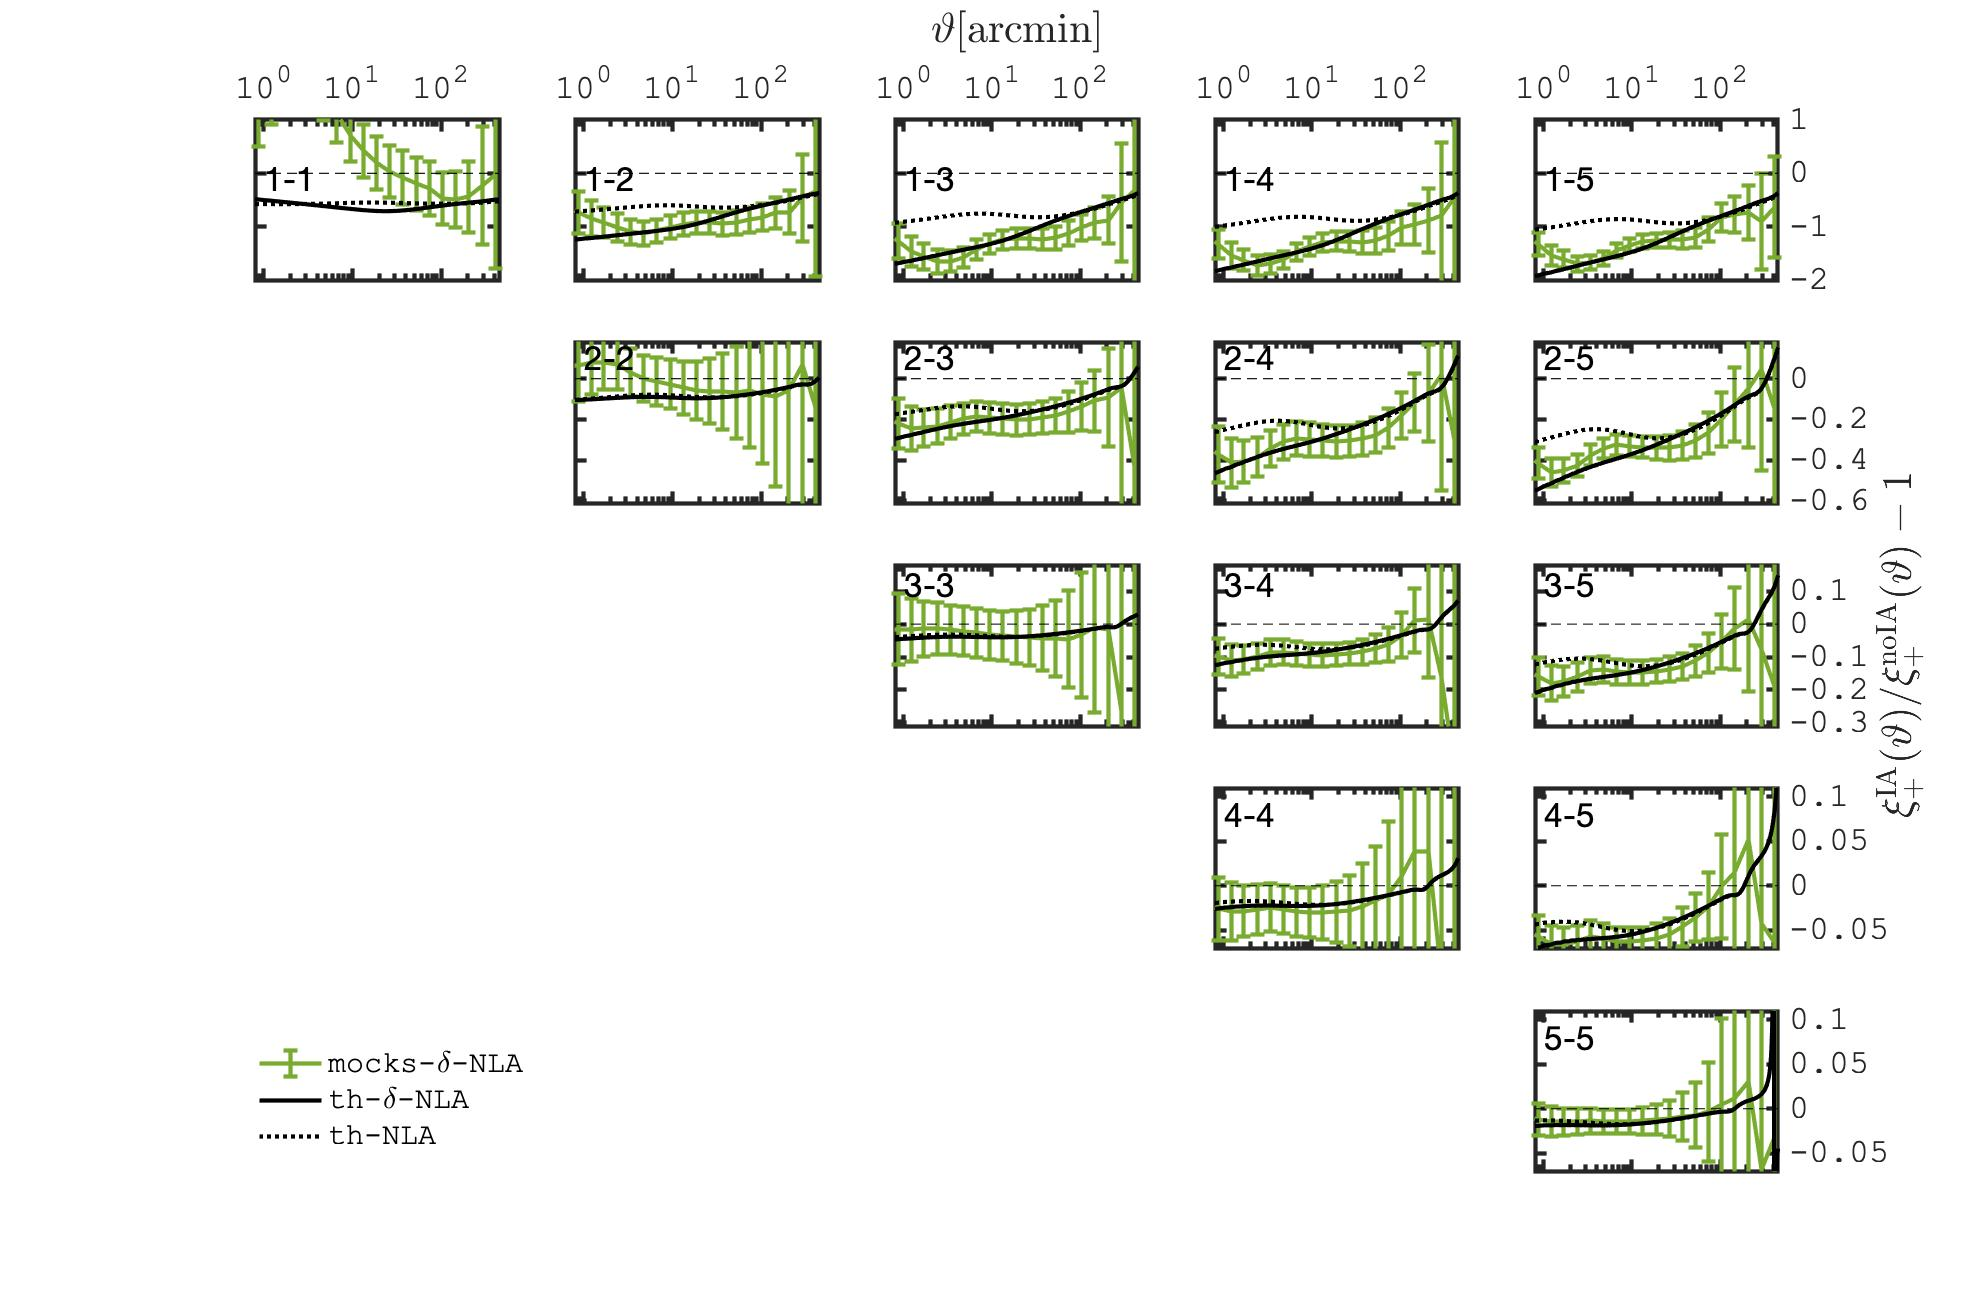
\includegraphics[width=\columnwidth]{graphs/frac_xip_IA1_skysim_deltaNLA_srd}
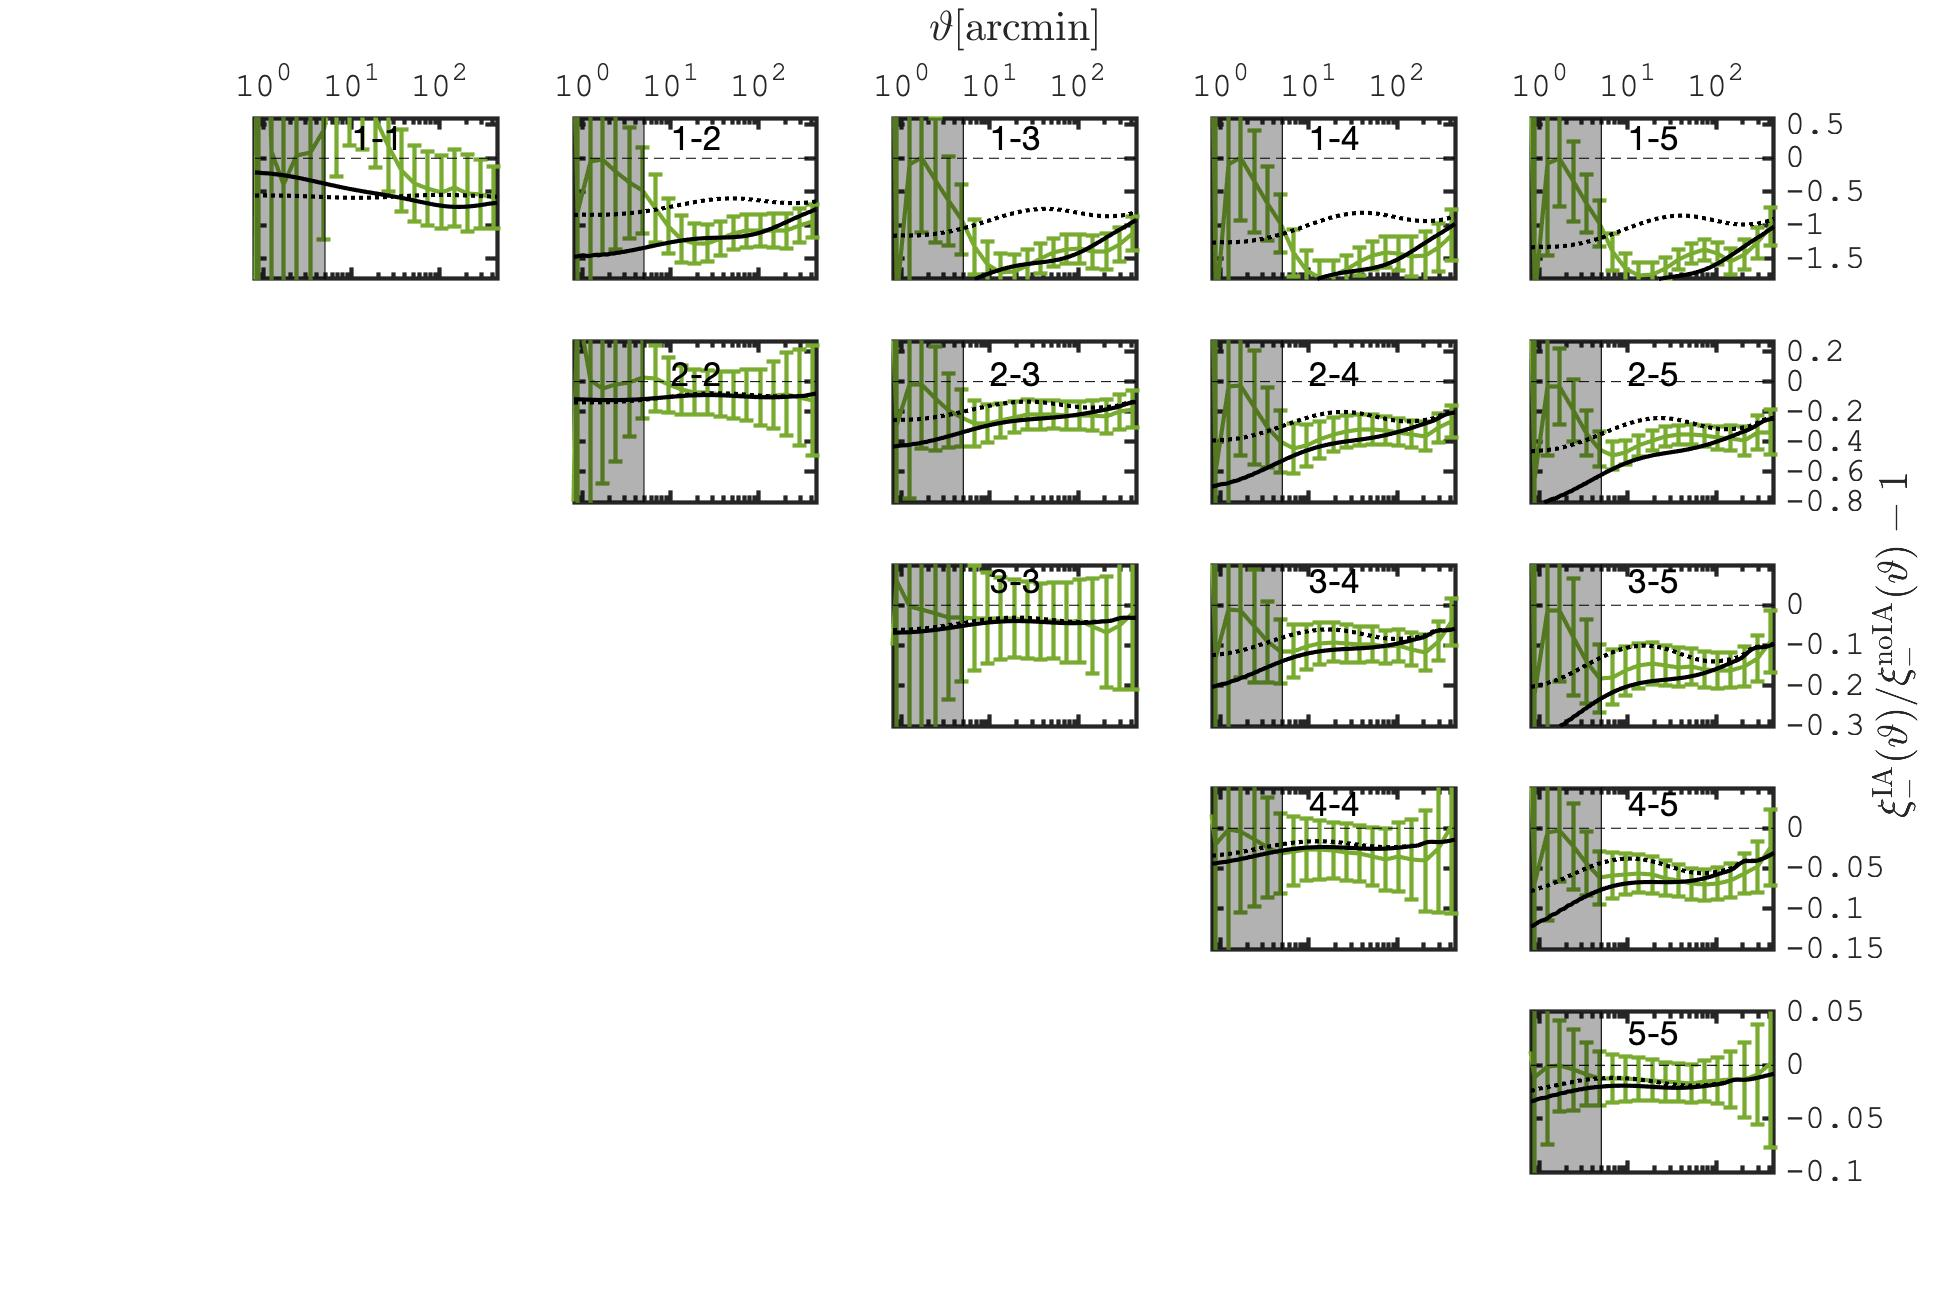
\includegraphics[width=\columnwidth]{graphs/frac_xim_IA1_skysim_deltaNLA_srd}
\caption{Same as Fig. \ref{fig:xi_NLA}, but for the $\delta$-NLA model with $A_{\rm IA}=1.0$ and $b_{\rm TA}=1.0$, and only for smoothing of 0.5$h^{-1}$Mpc. The dashed black lines show the NLA predictions to better highlight the differences.  }
\label{fig:xi_deltaNLA}
\end{figure*}



\begin{figure}
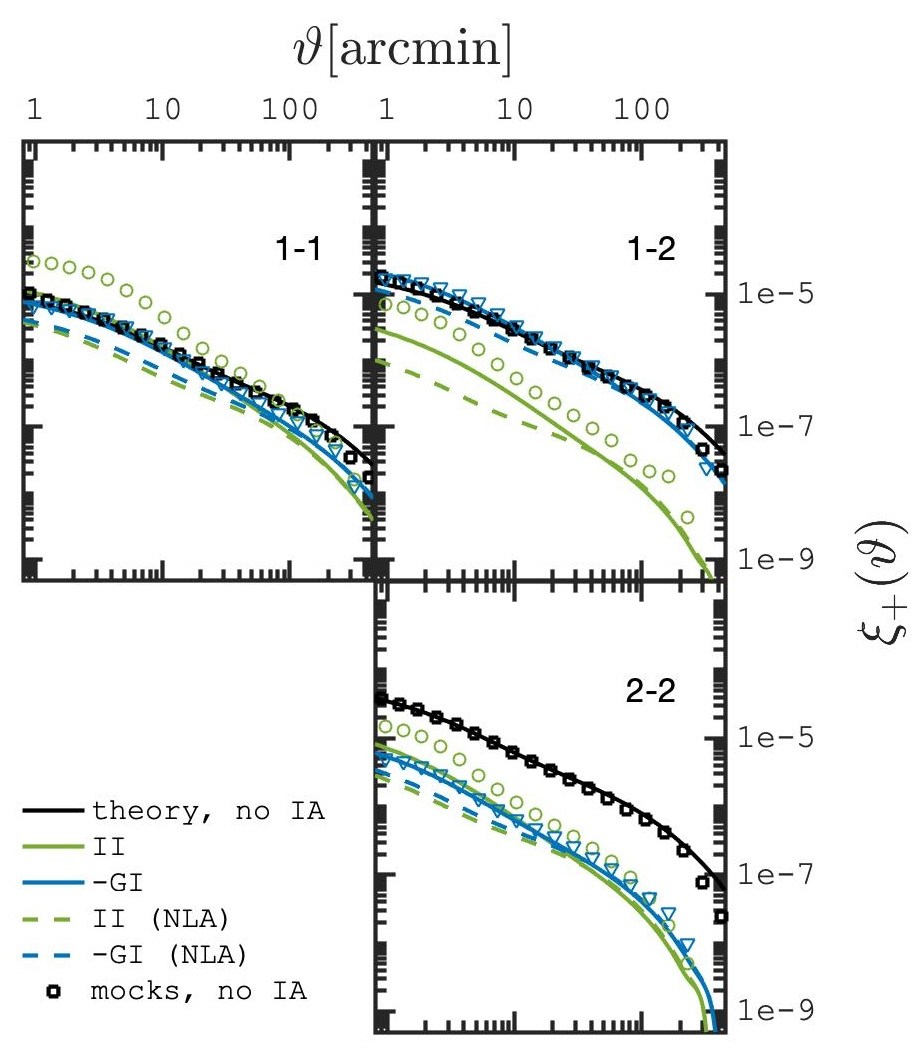
\includegraphics[width=\columnwidth]{graphs/xip_deltaNLA_bta1.jpg}
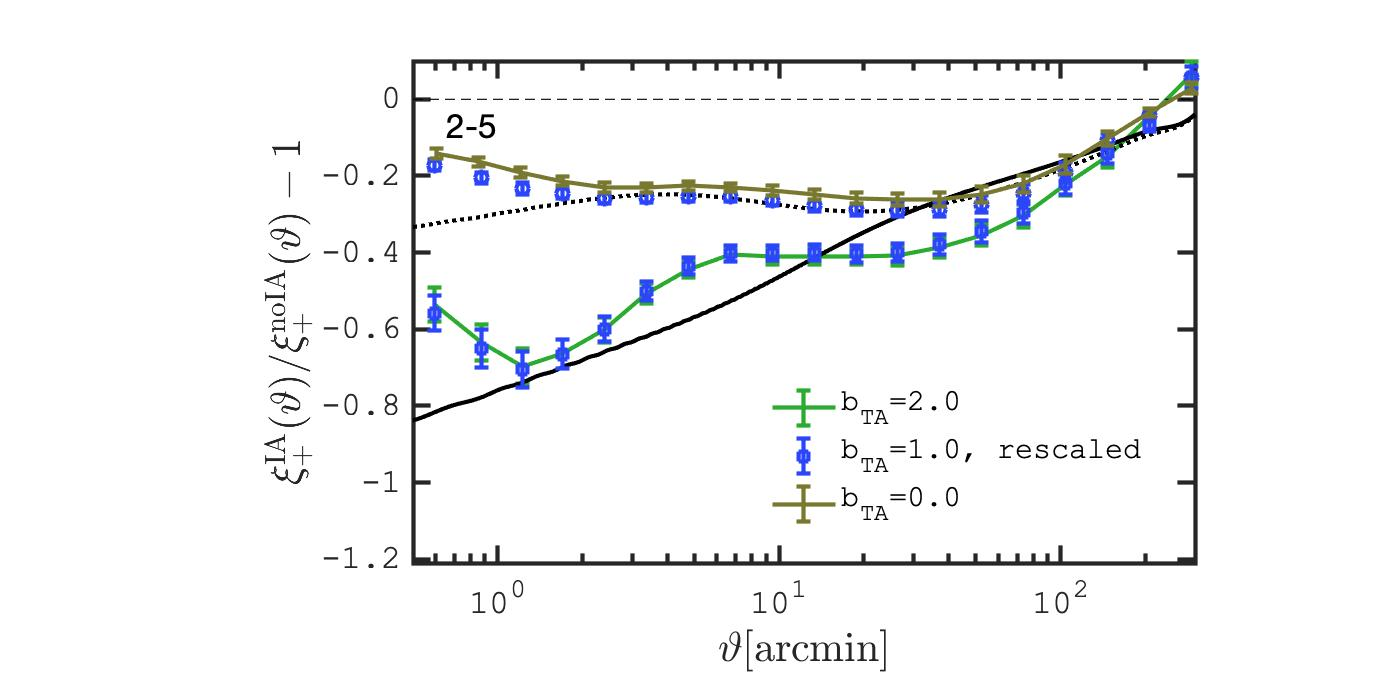
\includegraphics[width=\columnwidth]{graphs/frac_xip_bta1_rescaled}
\caption{Ratio between the shear correlation functions with and without IA in tomographic bin combination 2-5. The brown and green symbols show measurements from simulations constructed with $b_{\rm TA}$ = 0.0 and 2.0 respectively,  the black solid and dotted lines shown their predictions, while the blue symbols are obtained by rescaling $b_{\rm TA}$ = 1.0 simulations using Eq. \ref{eq:bta_rescale}.  }
\label{fig:xi_deltaNLA_rescaled}
\end{figure}


We verified that it works equally well for $b_{\rm TA}$ = 1.0 and 2.0.

%------------------------------

Using this, we $b_{\rm TA}$-rescale our $b_{\rm TA}=1.0$ mock to $b_{\rm TA}=2.0$ and to $0.0$ mocks. Results are shown in Fig. \ref{fig:xi_deltaNLA_rescaled} for one of the tomographic bin. It works reasonably well, but lower redshift are less accurate due to the increased  shot noise (not shown), hence we do not recommend using this.

%------------------------------
\subsection{TT model}
\label{subsec:TT}

See Fig. \ref{fig:xi_TT}

\begin{figure*}
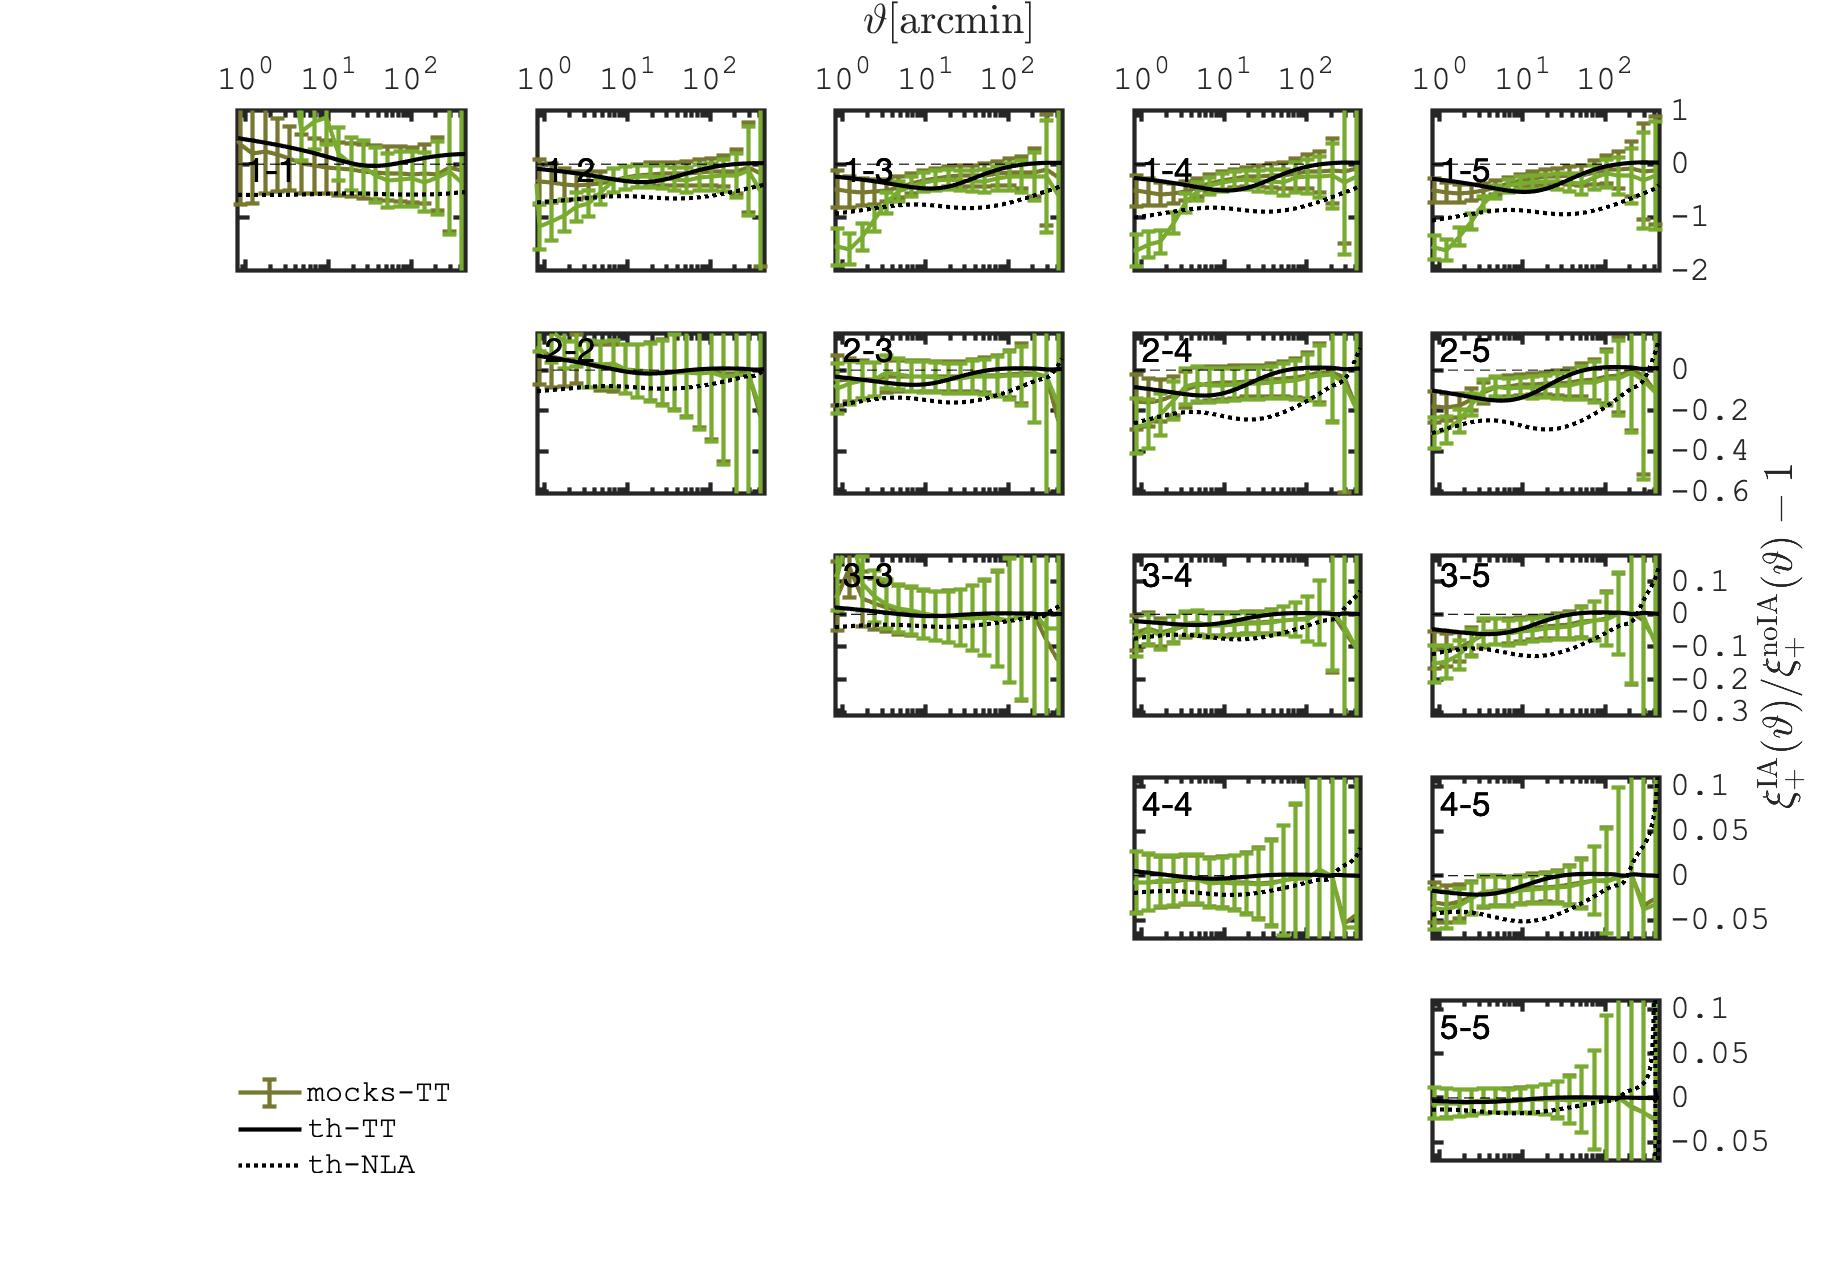
\includegraphics[width=\columnwidth]{graphs/frac_xip_IA1_skysim_TT_srd.jpg}
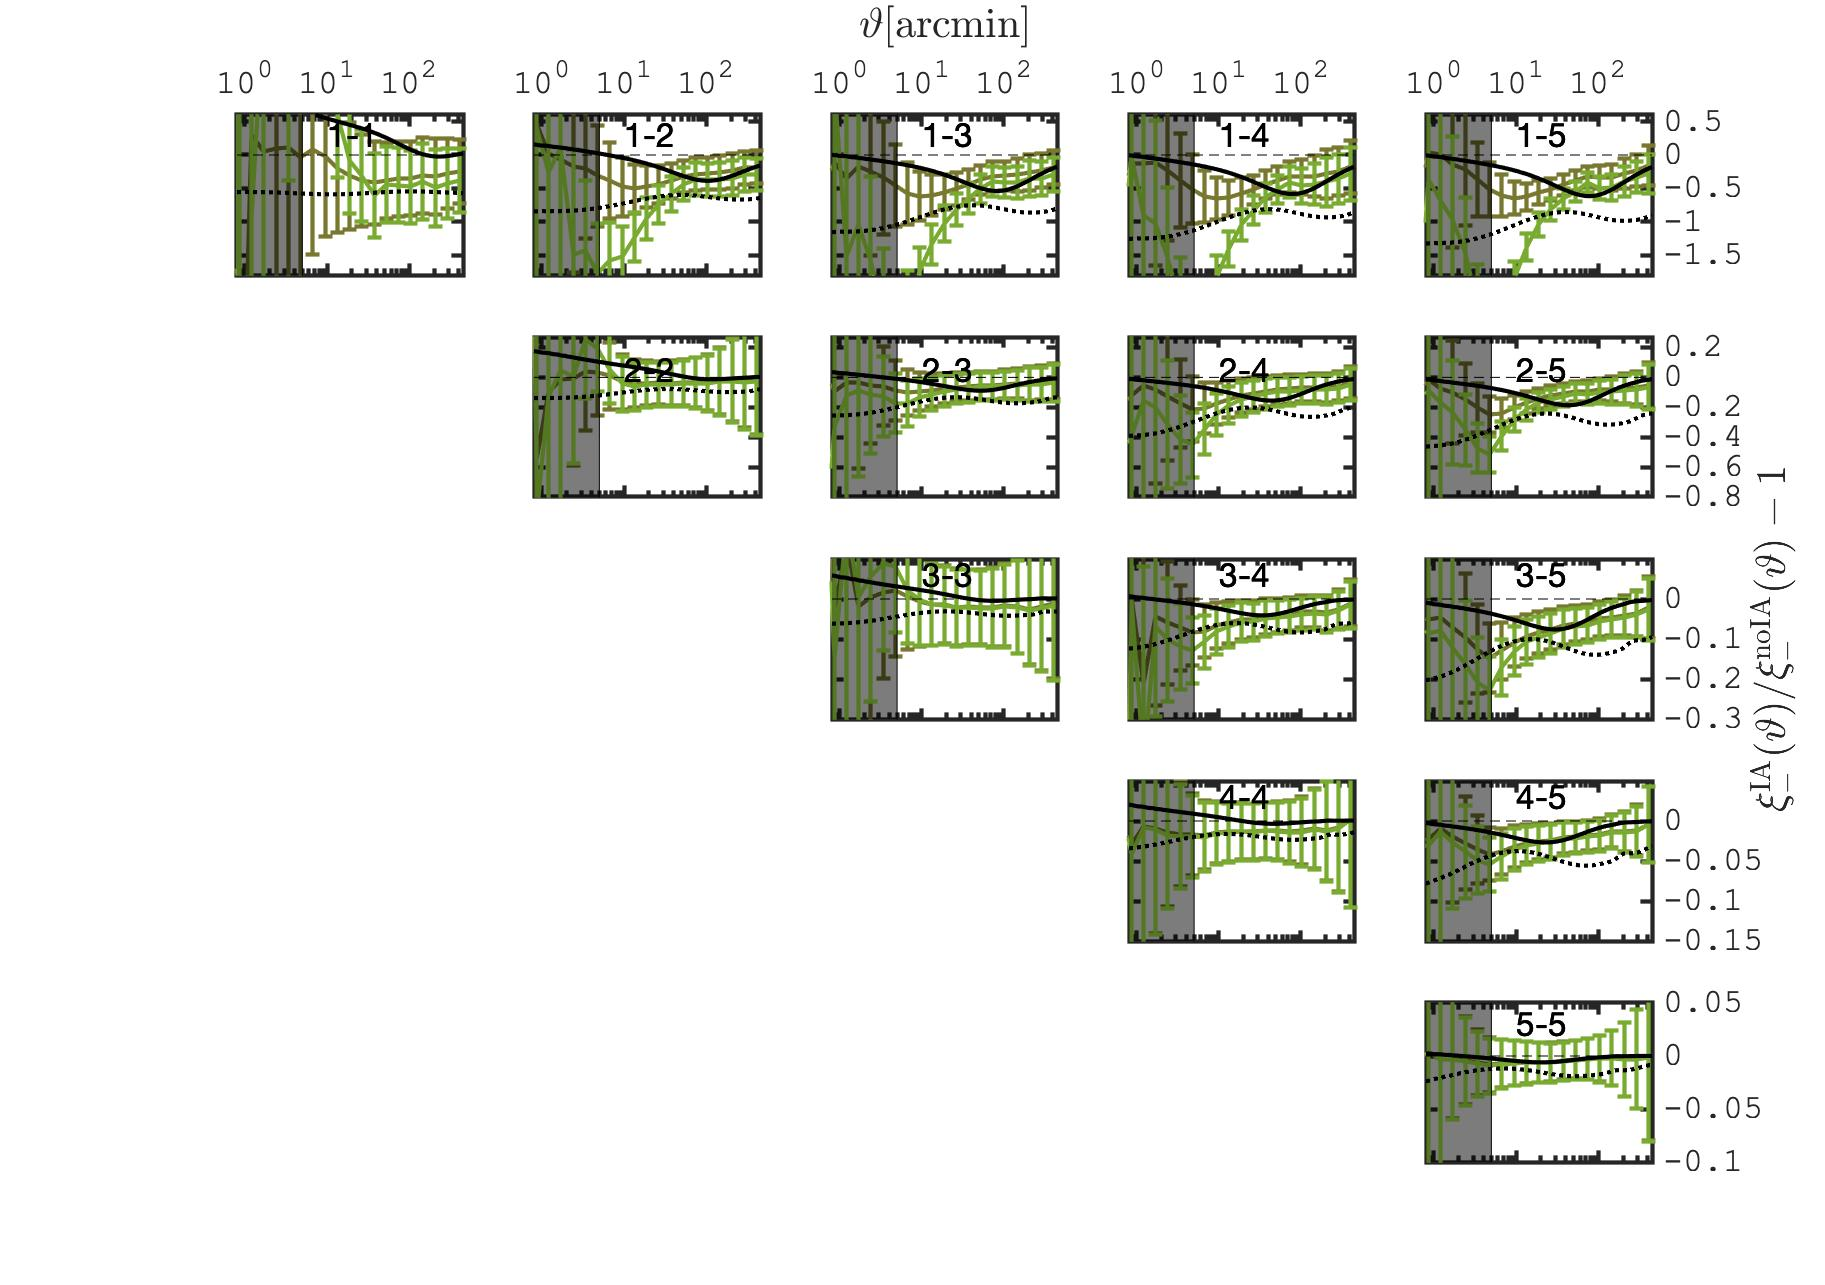
\includegraphics[width=\columnwidth]{graphs/frac_xim_IA1_skysim_TT_srd.jpg}
\caption{Same as Fig. \ref{fig:xi_NLA}, but for the TT model with $A_2=1.0$. Here, the dashed black lines show the NLA predictions to better highlight the differences. }
\label{fig:xi_TT}
\end{figure*}

\begin{figure*}
%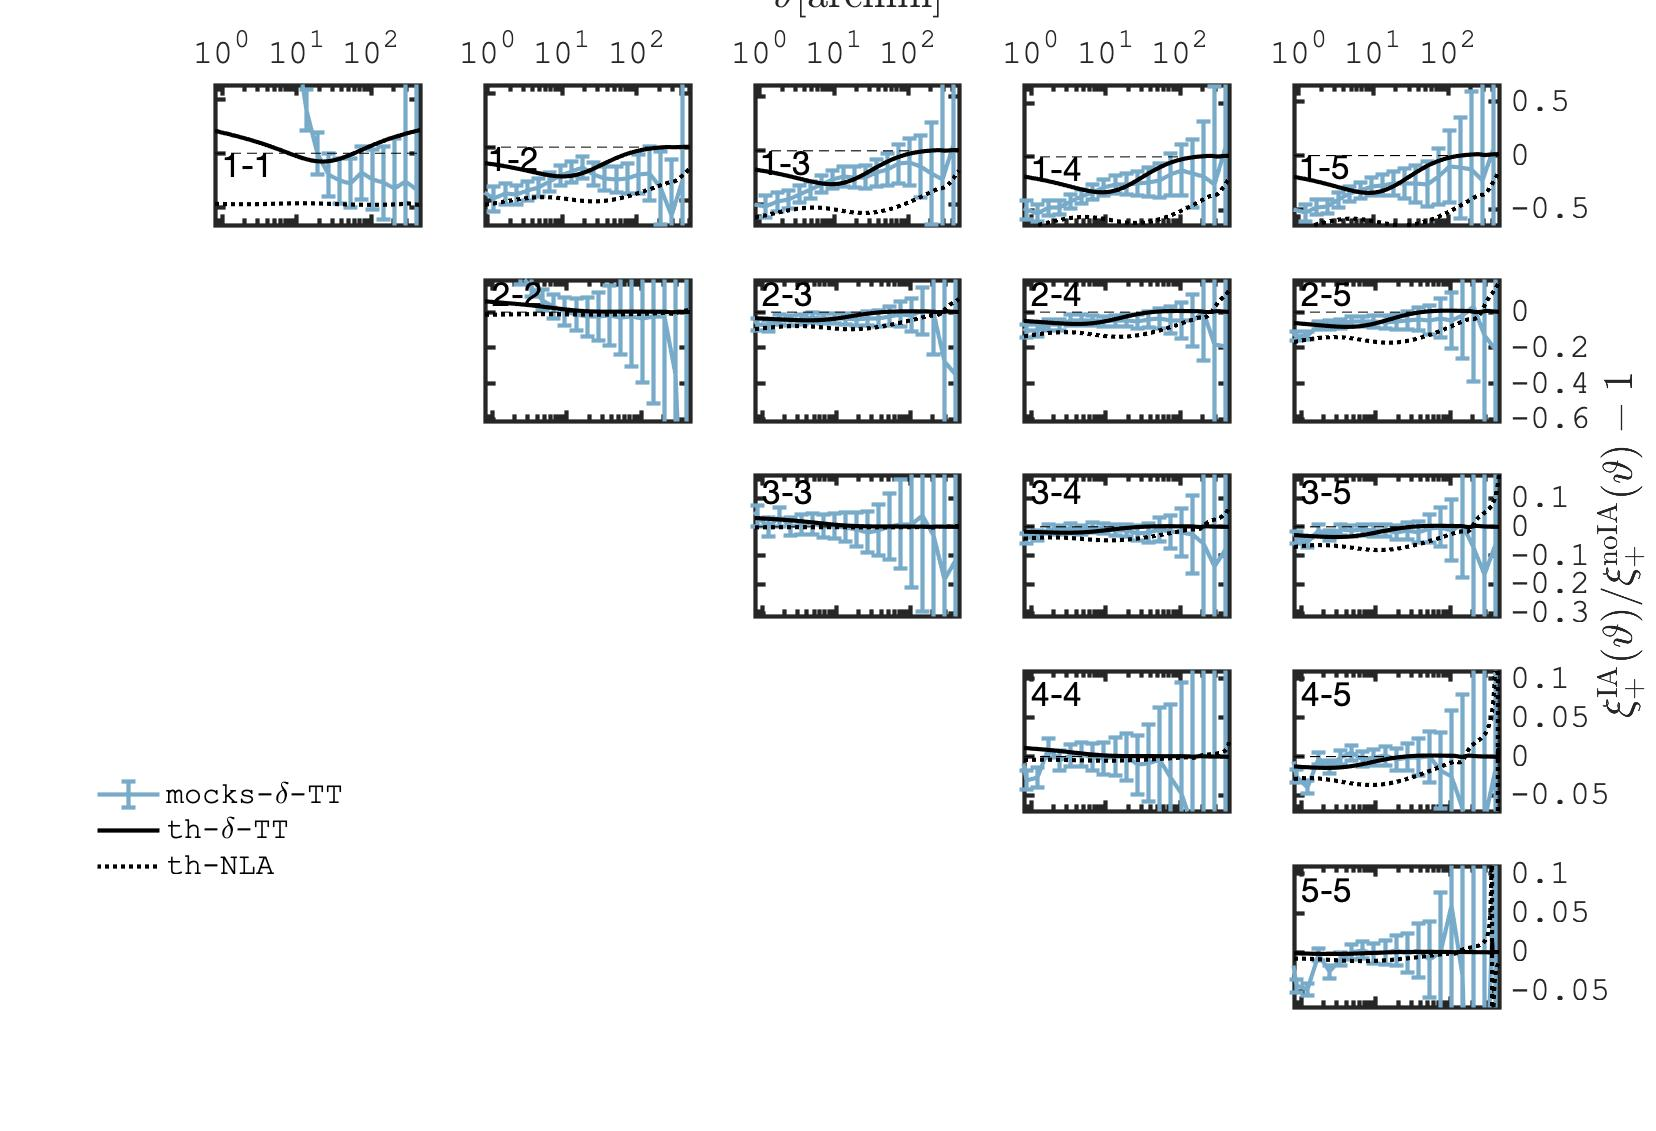
\includegraphics[width=\columnwidth]{graphs/frac_xip_C2_m1_skysim_deltaTT}
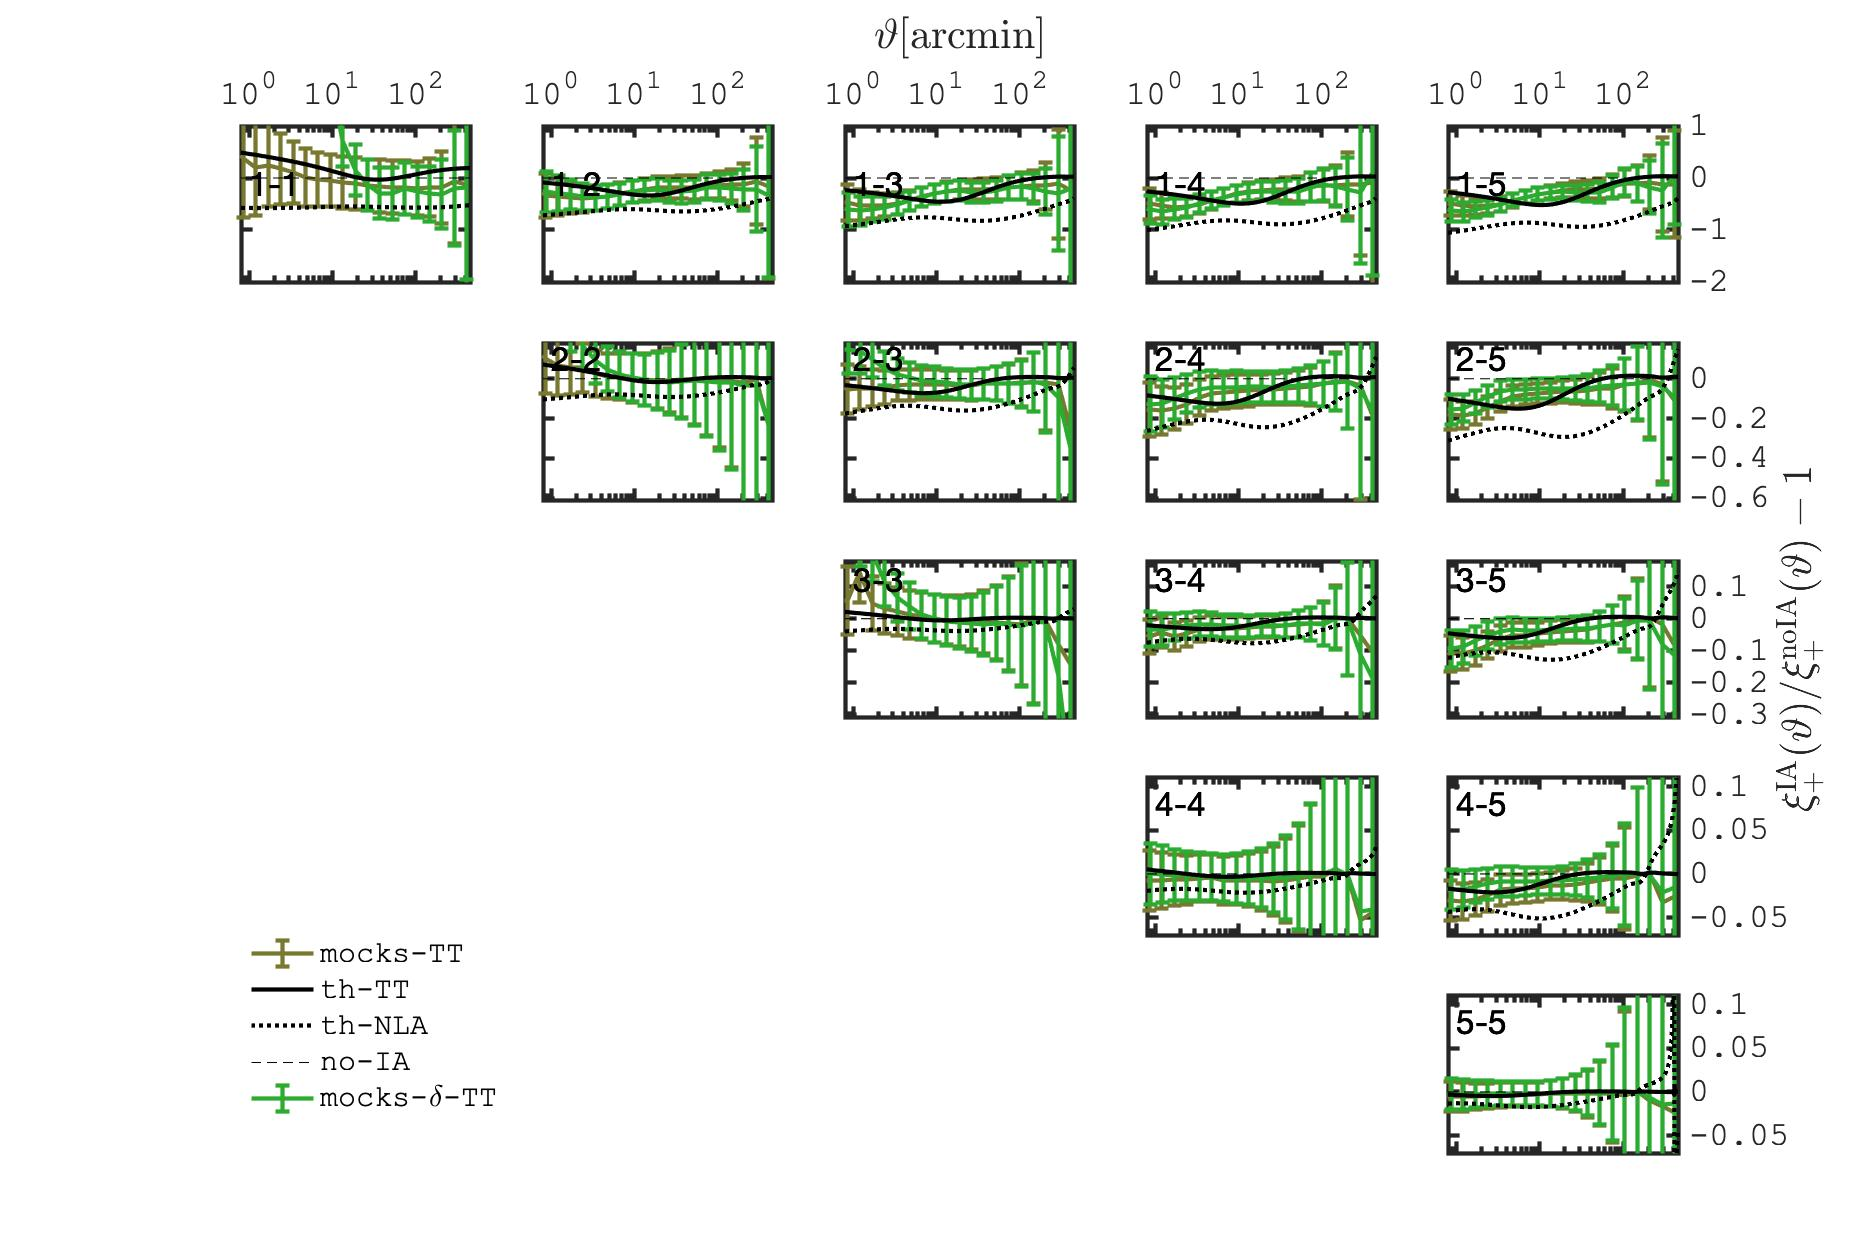
\includegraphics[width=\columnwidth]{graphs/frac_xip_IA1_skysim_deltaTT_srd.jpg}
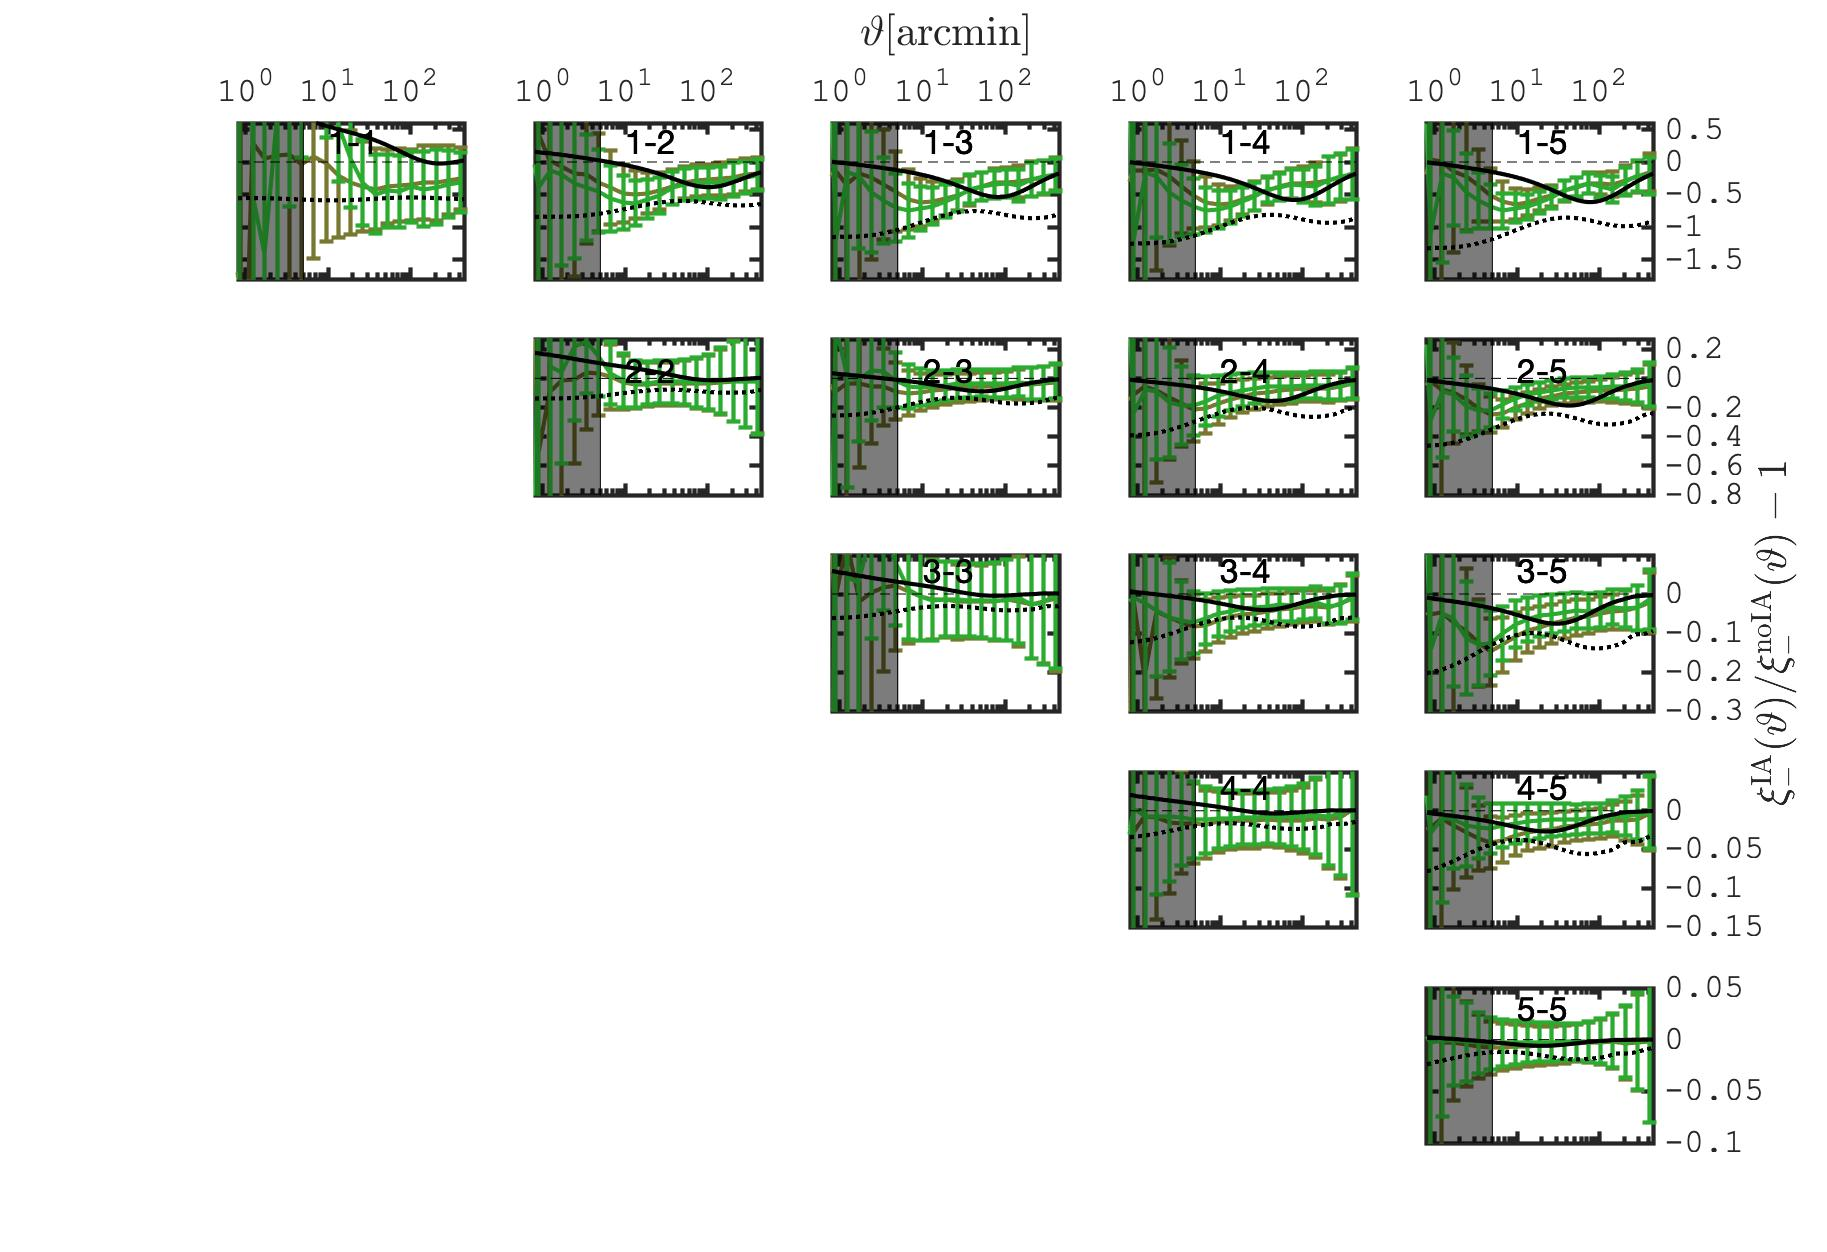
\includegraphics[width=\columnwidth]{graphs/frac_xim_IA1_skysim_deltaTT_srd.jpg}
\caption{Same as Fig. \ref{fig:xi_deltaNLA}, but comparing the TT and the $\delta$-TT models, with $A_2=1.0$, $b_{\rm TA}$ = 1.0, and only for smoothing of 0.5$h^{-1}$Mpc. }
\label{fig:xi_deltaTT}
\end{figure*}



To match the theory, we need to apply the following calibration: $\epsilon^{\rm IA, TT}(z<0.5) \rightarrow \epsilon^{\rm IA, TT} /2.5$.

%------------------------------
\subsection{$\delta$-TT model}
\label{subsec:TT}

See Fig. \ref{fig:xi_deltaTT}

To match the TT theory, we need to apply the following calibration: $\epsilon^{\rm IA, TT}(z<0.5) \rightarrow \epsilon^{\rm IA, TT} /5.0$, followed by $\epsilon^{\rm IA, TT} \rightarrow \epsilon^{\rm IA, TT}/7.0$.

%------------------------------
\subsection{HOD-NLA model}
\label{subsec:HOD}


%--------------
\begin{figure*}
%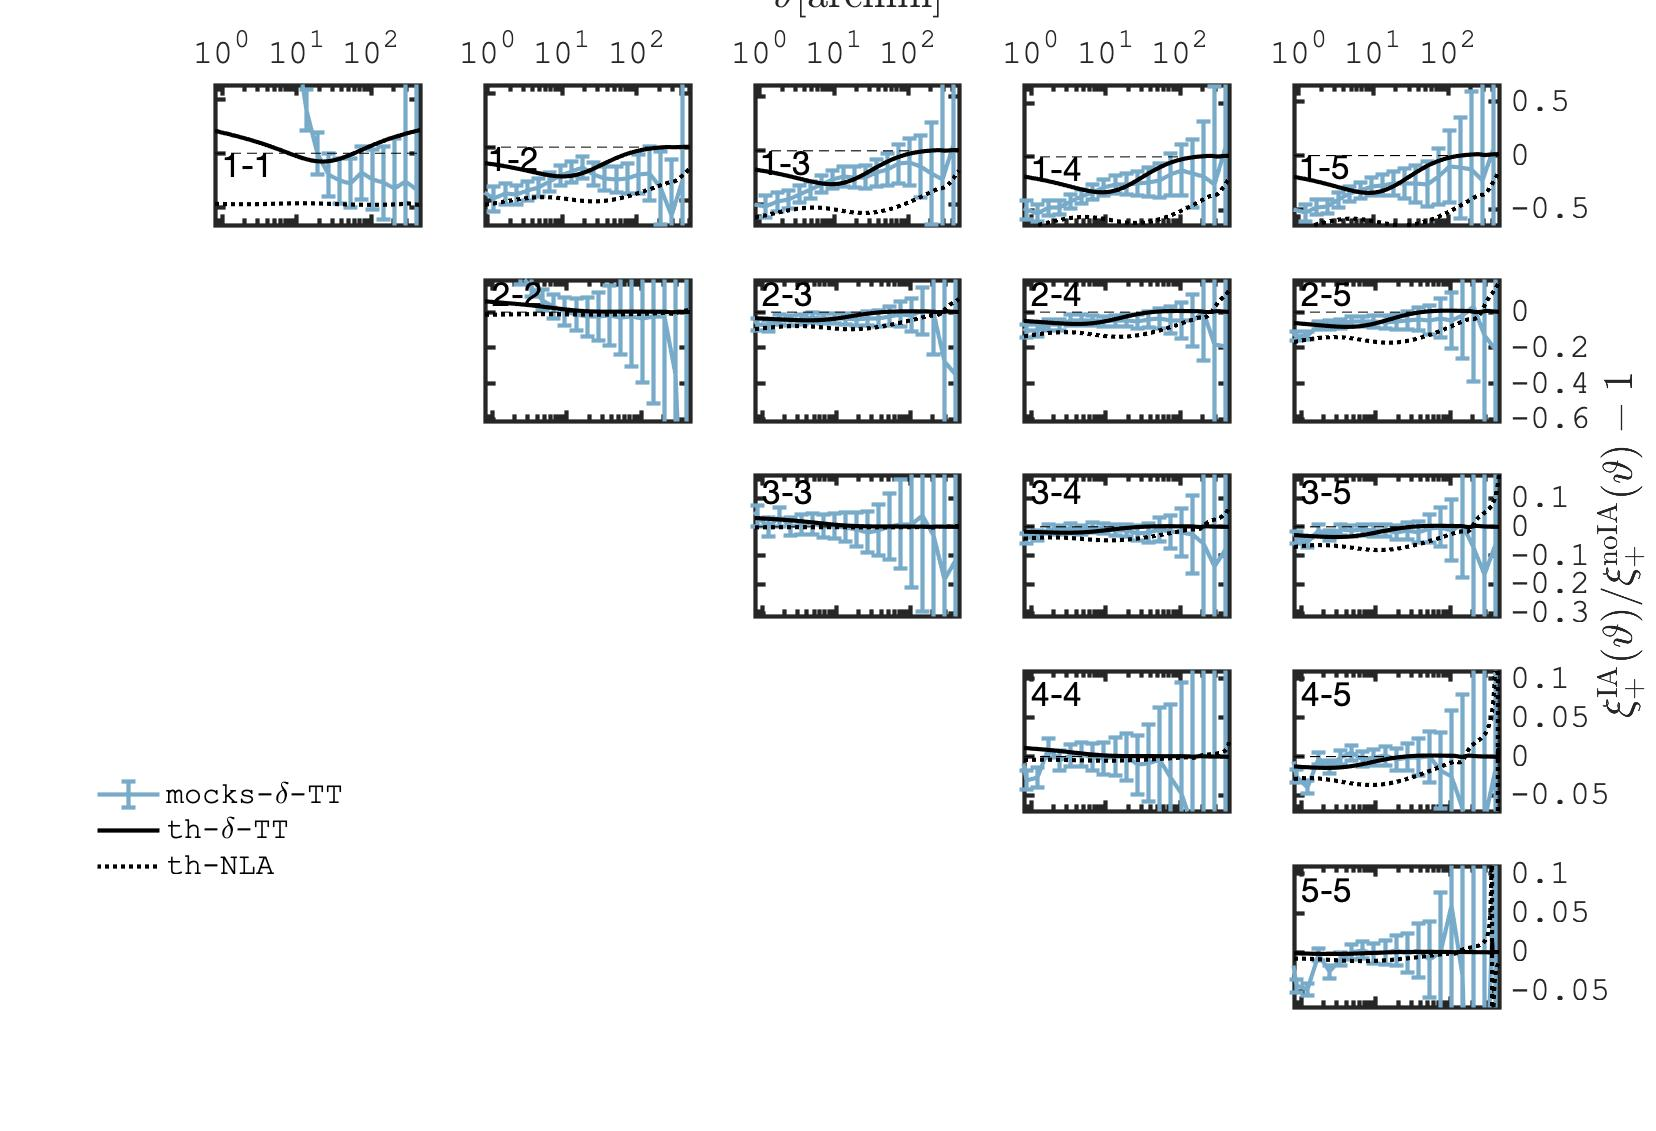
\includegraphics[width=\columnwidth]{graphs/frac_xip_C2_m1_skysim_deltaTT}
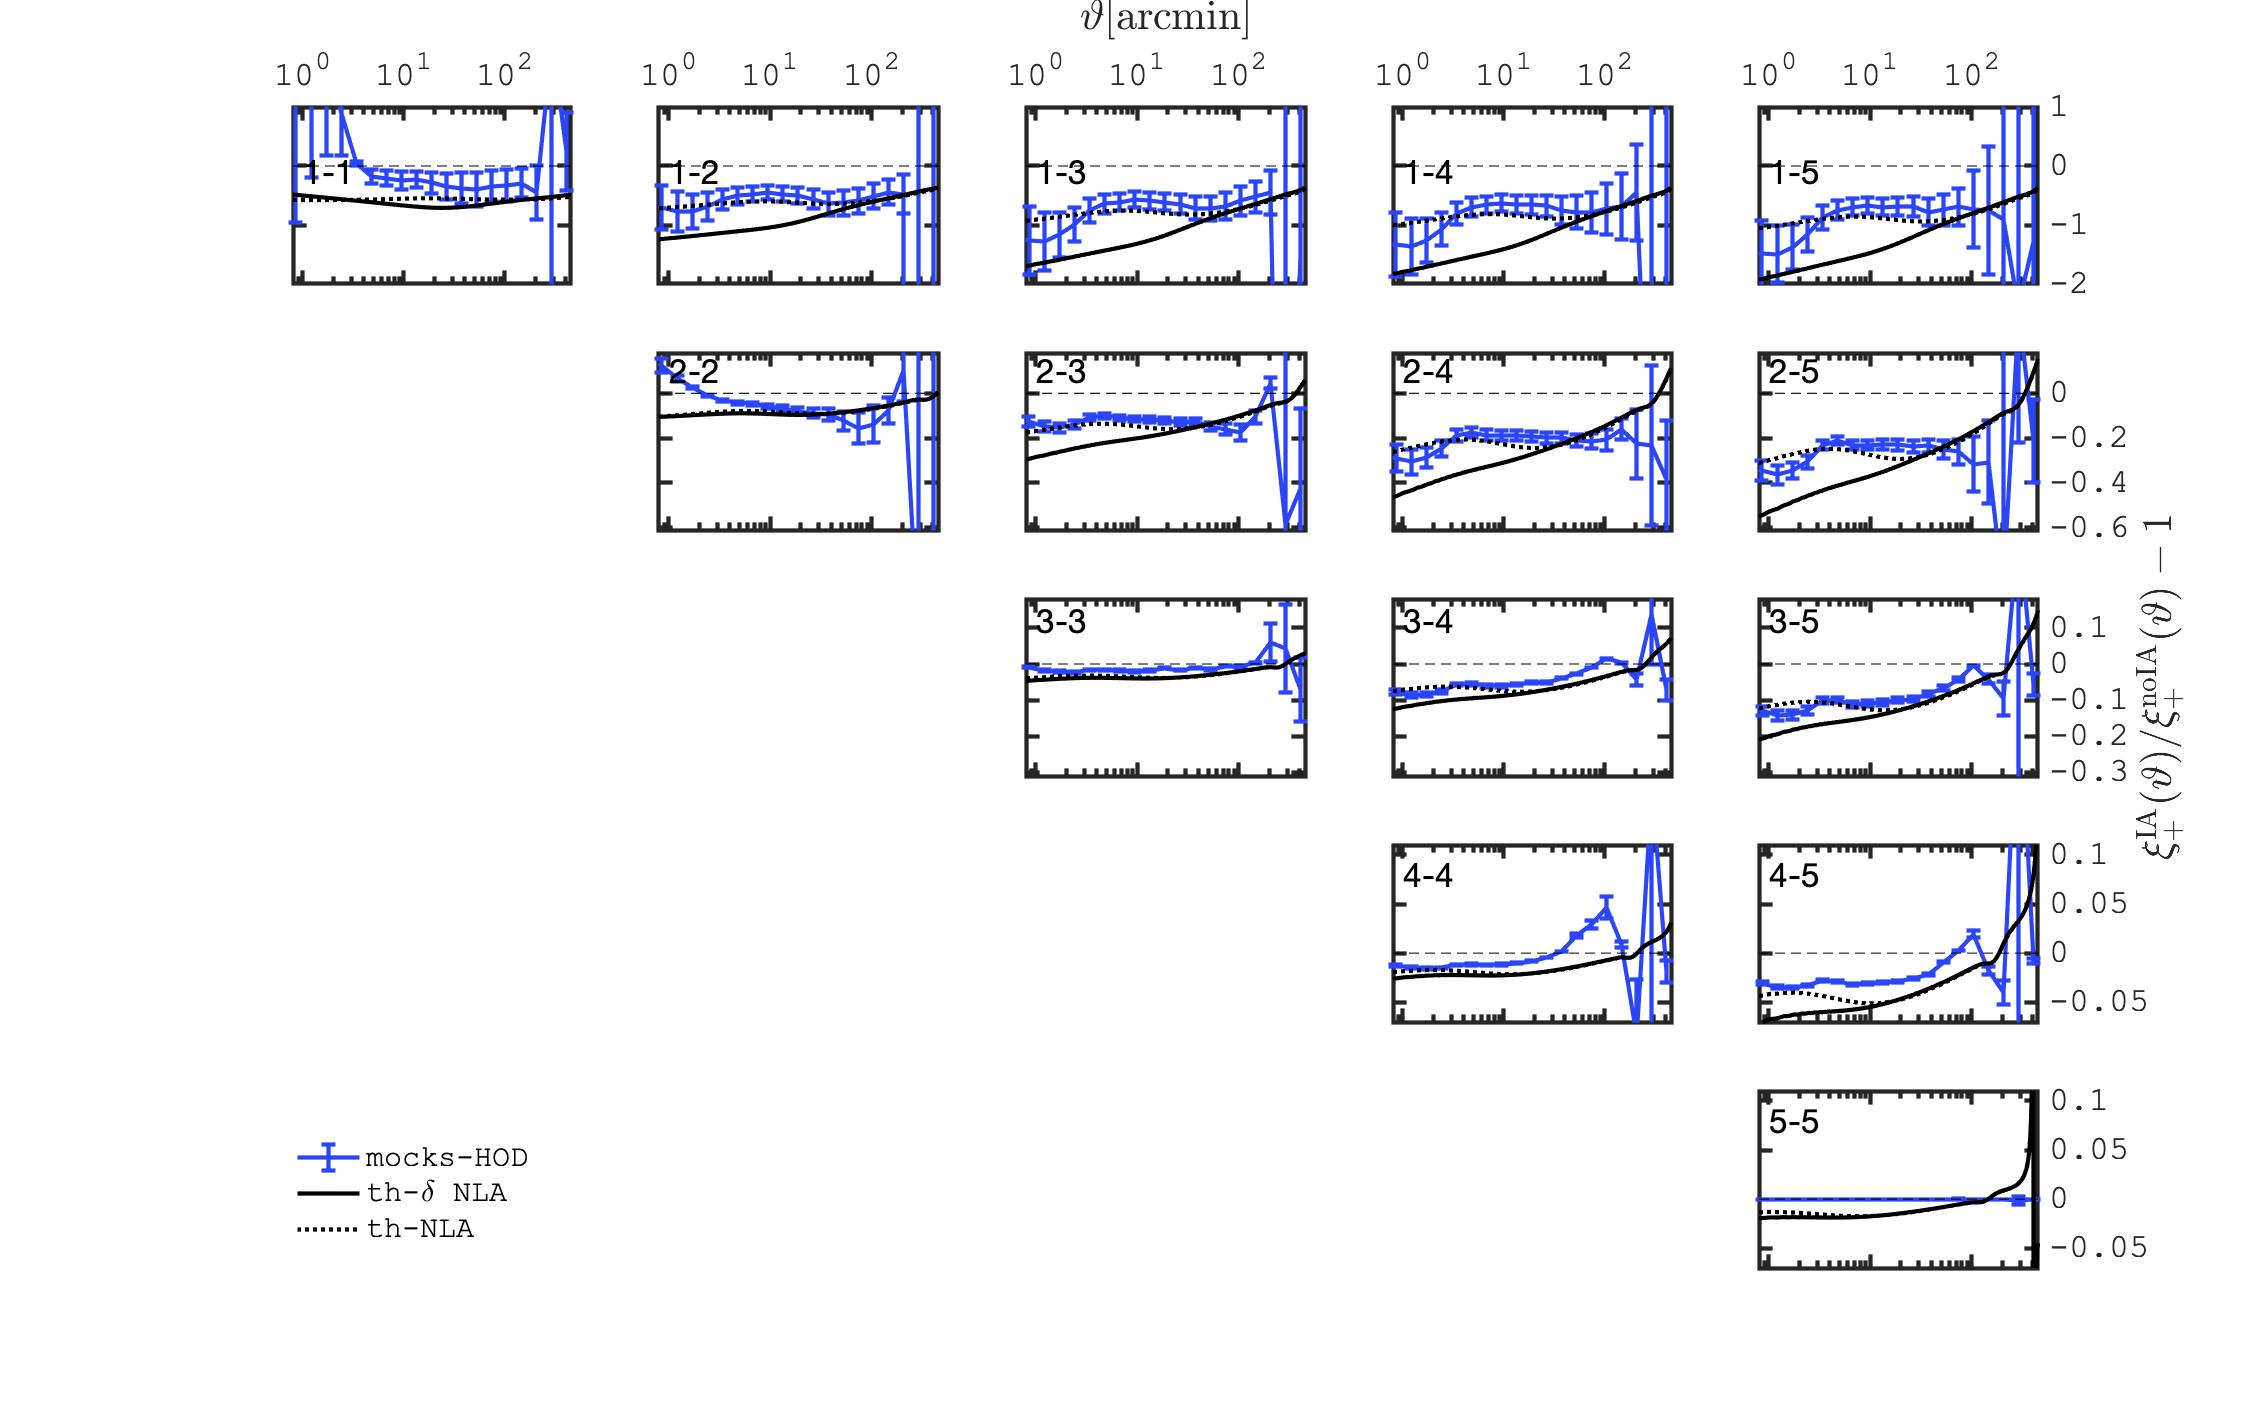
\includegraphics[width=\columnwidth]{graphs/frac_xip_sims_HOD.jpg}
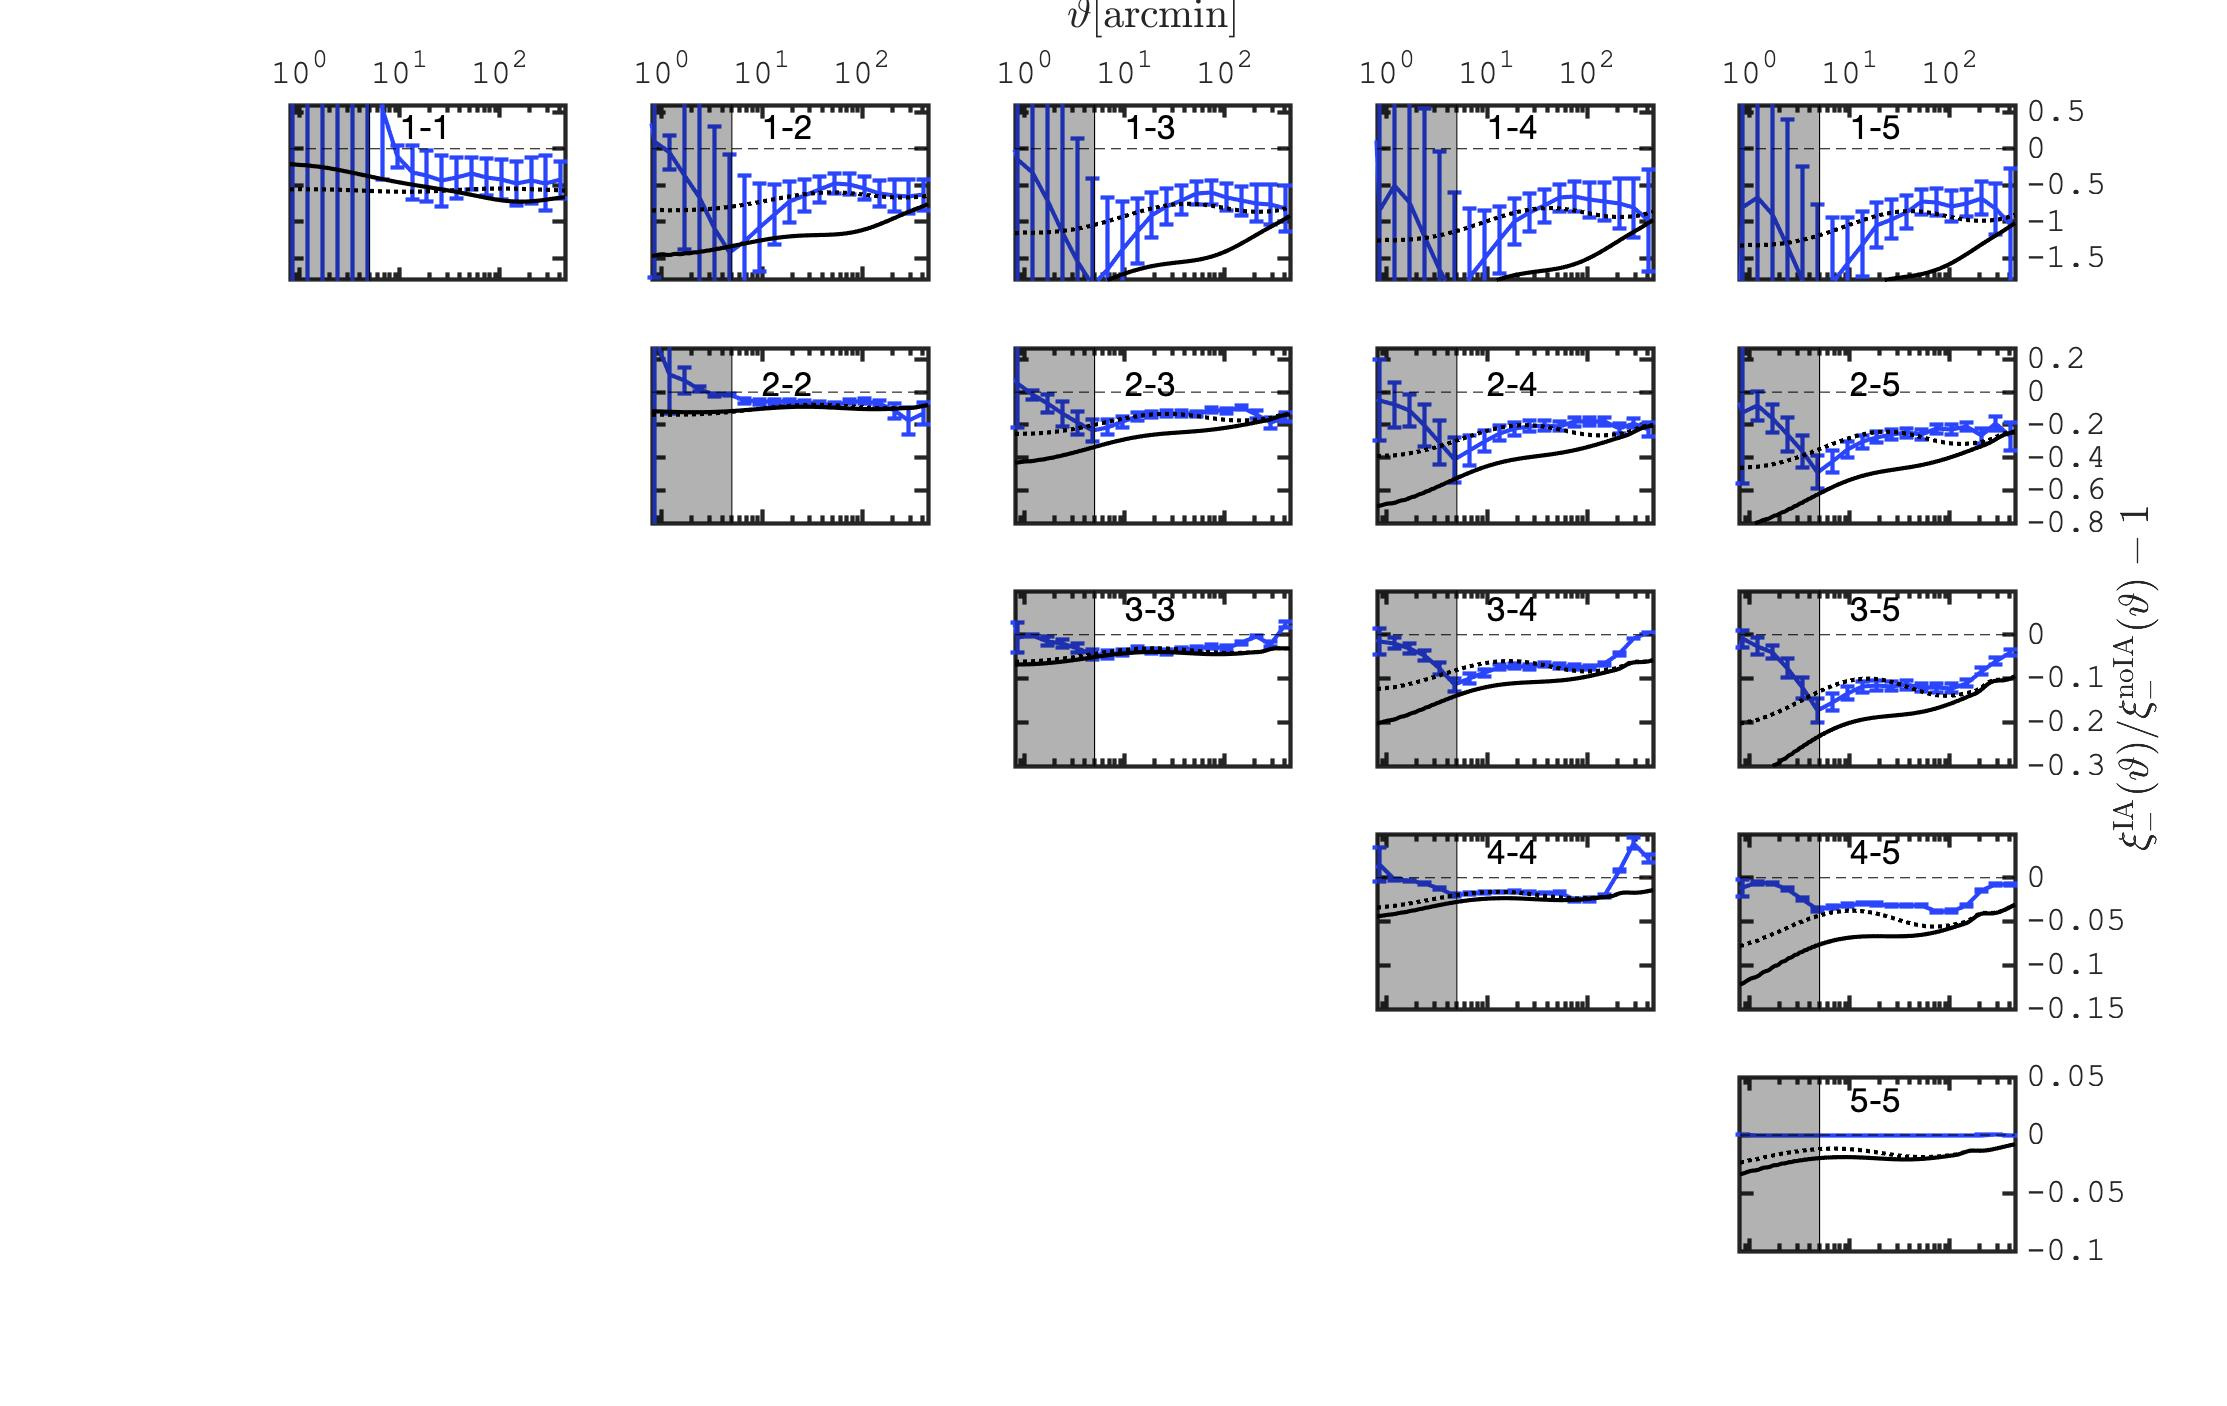
\includegraphics[width=\columnwidth]{graphs/frac_xim_sims_HOD.jpg}
\caption{Same as Fig. \ref{fig:xi_deltaNLA}, but showing the HOD galaxies with shapes linearly coupled with the tidal field. }
\label{fig:xi_HOD}
\end{figure*}

%--------------
\begin{figure*}
%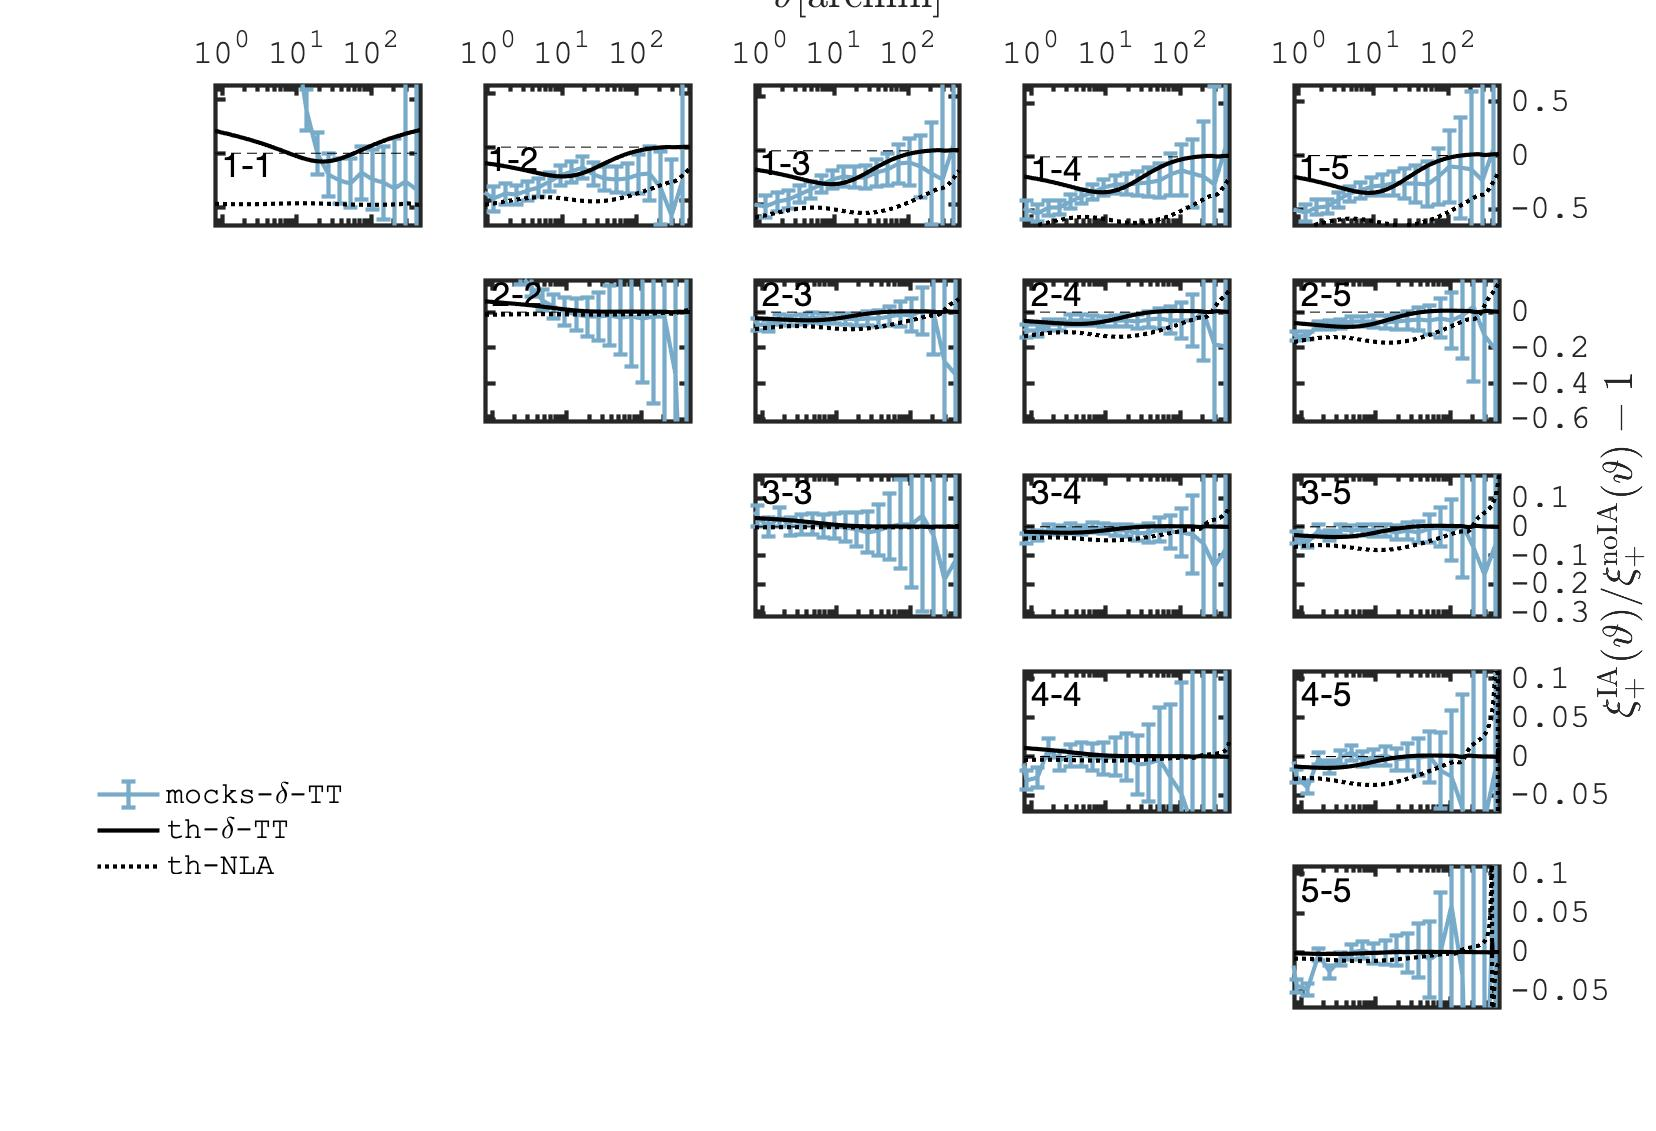
\includegraphics[width=\columnwidth]{graphs/frac_xip_C2_m1_skysim_deltaTT}
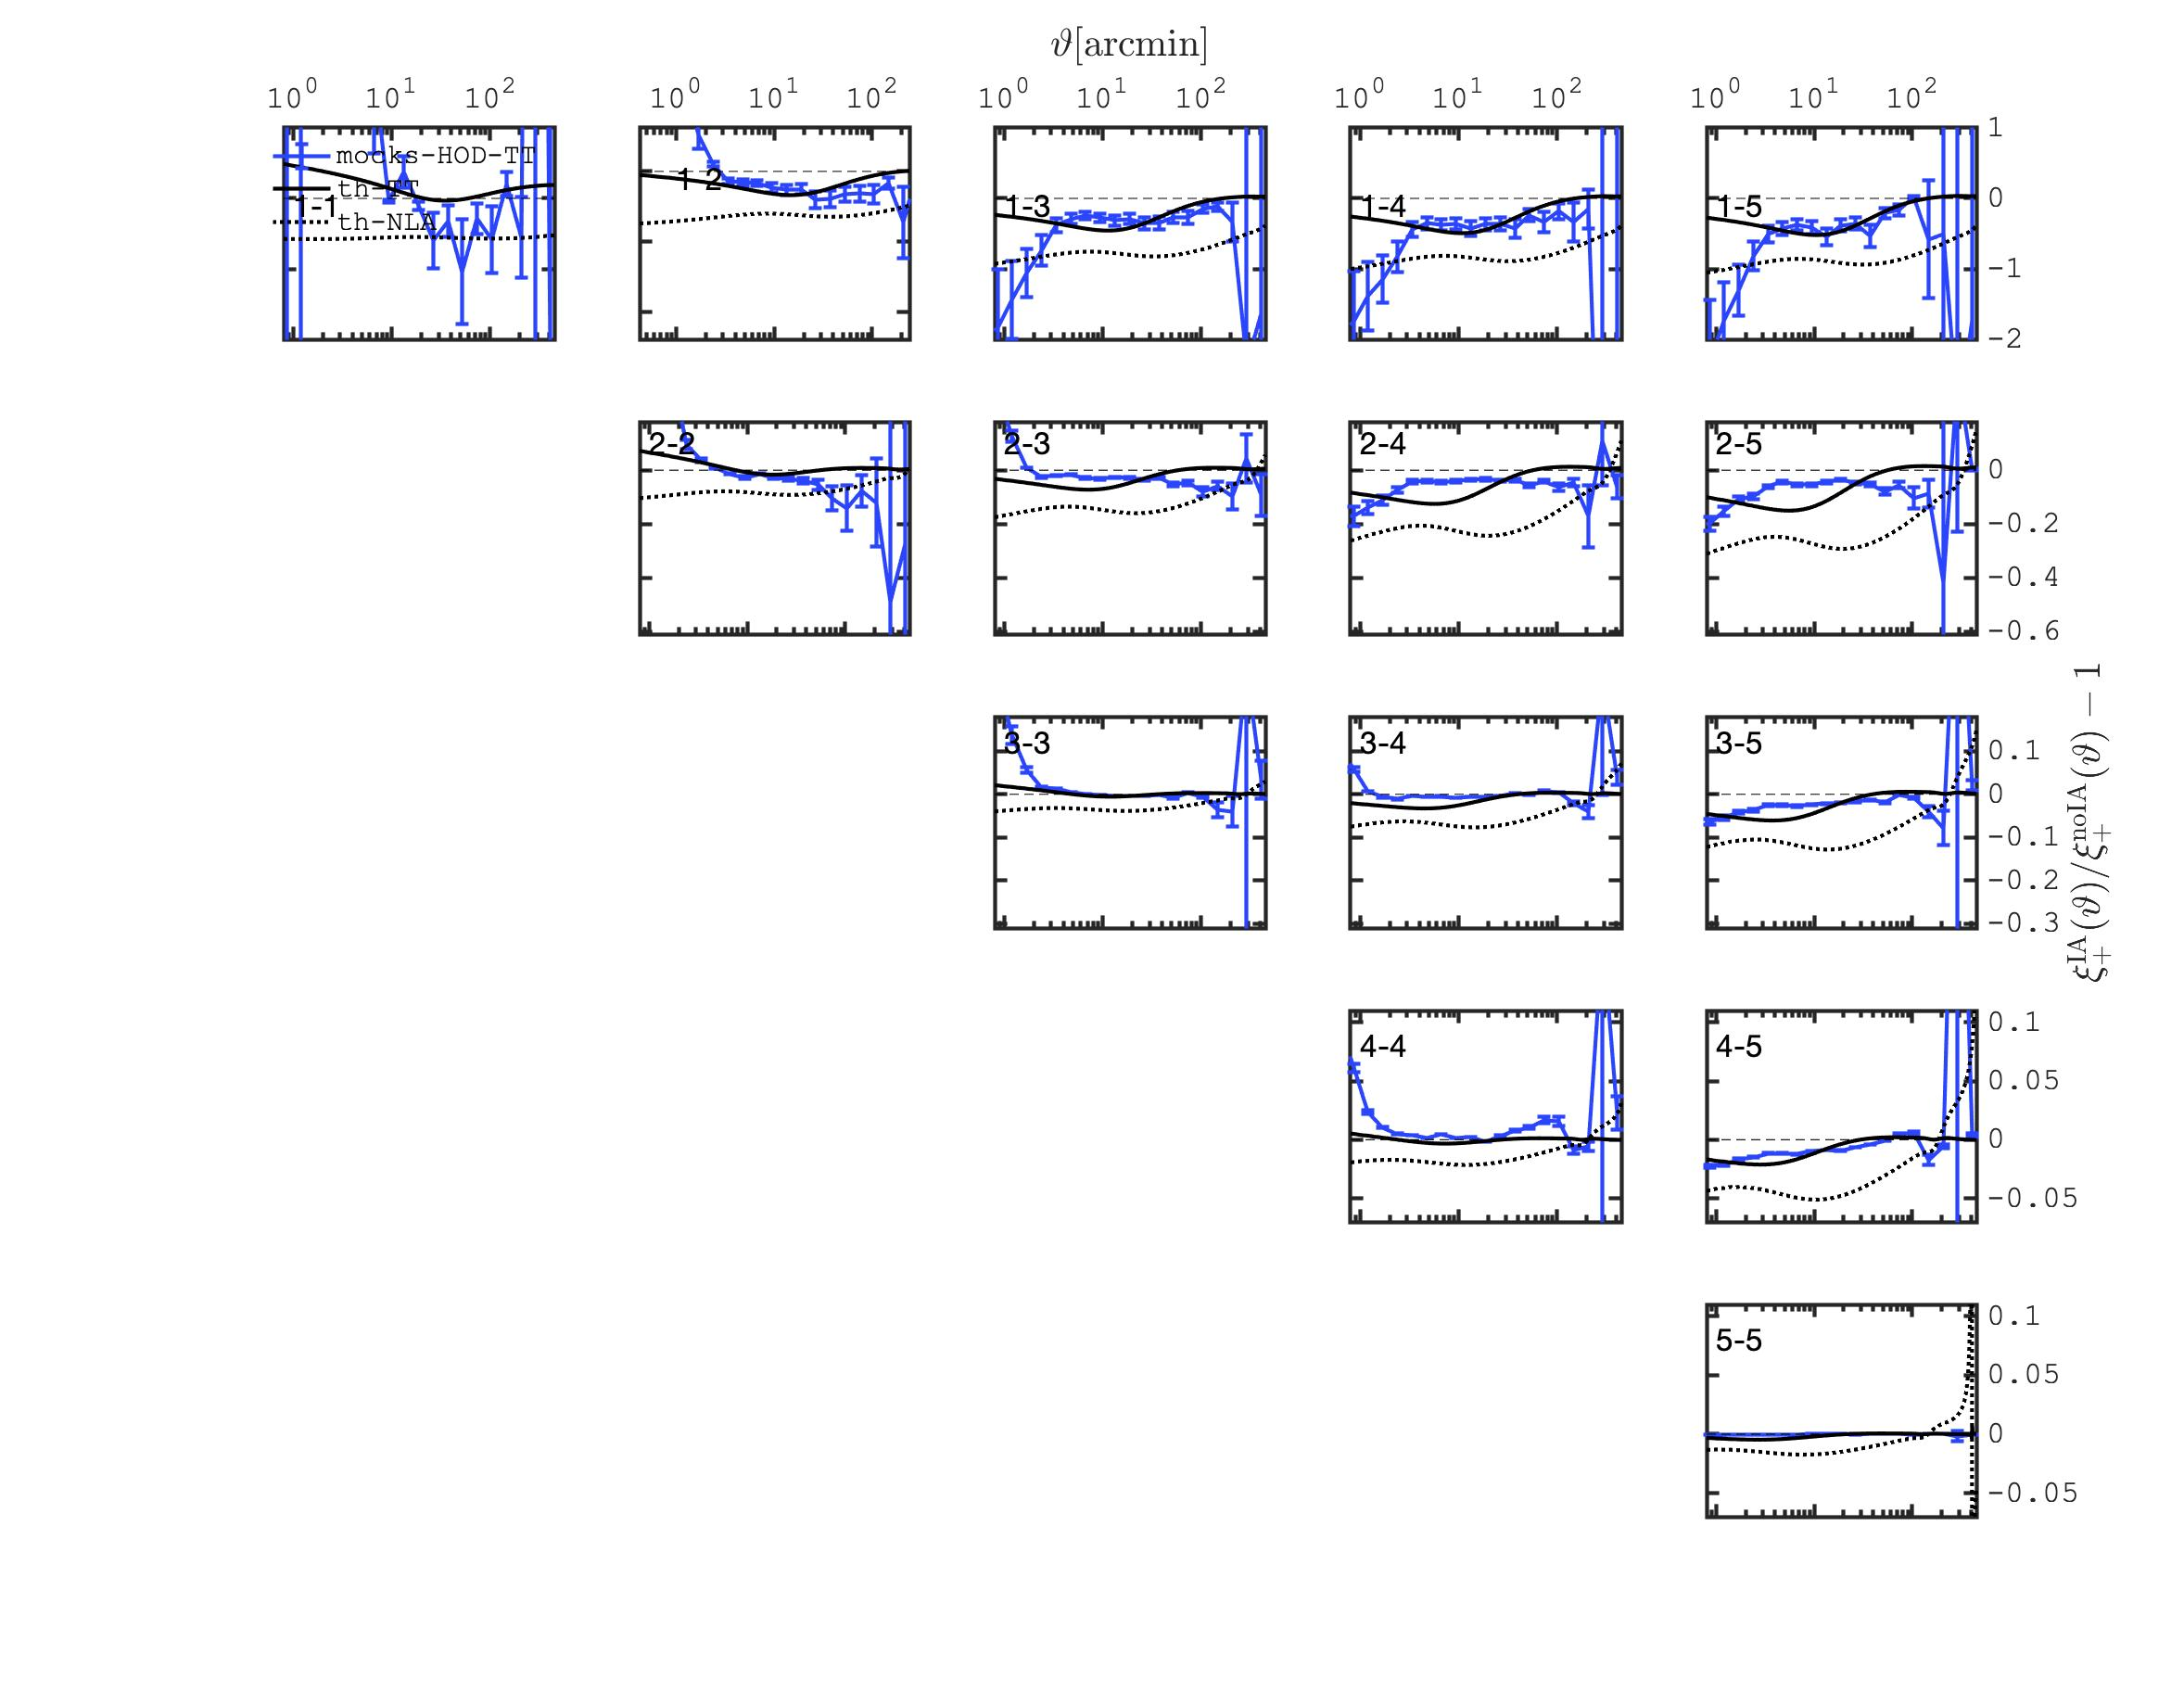
\includegraphics[width=\columnwidth]{graphs/frac_xip_sims_HOD_TT.jpg}
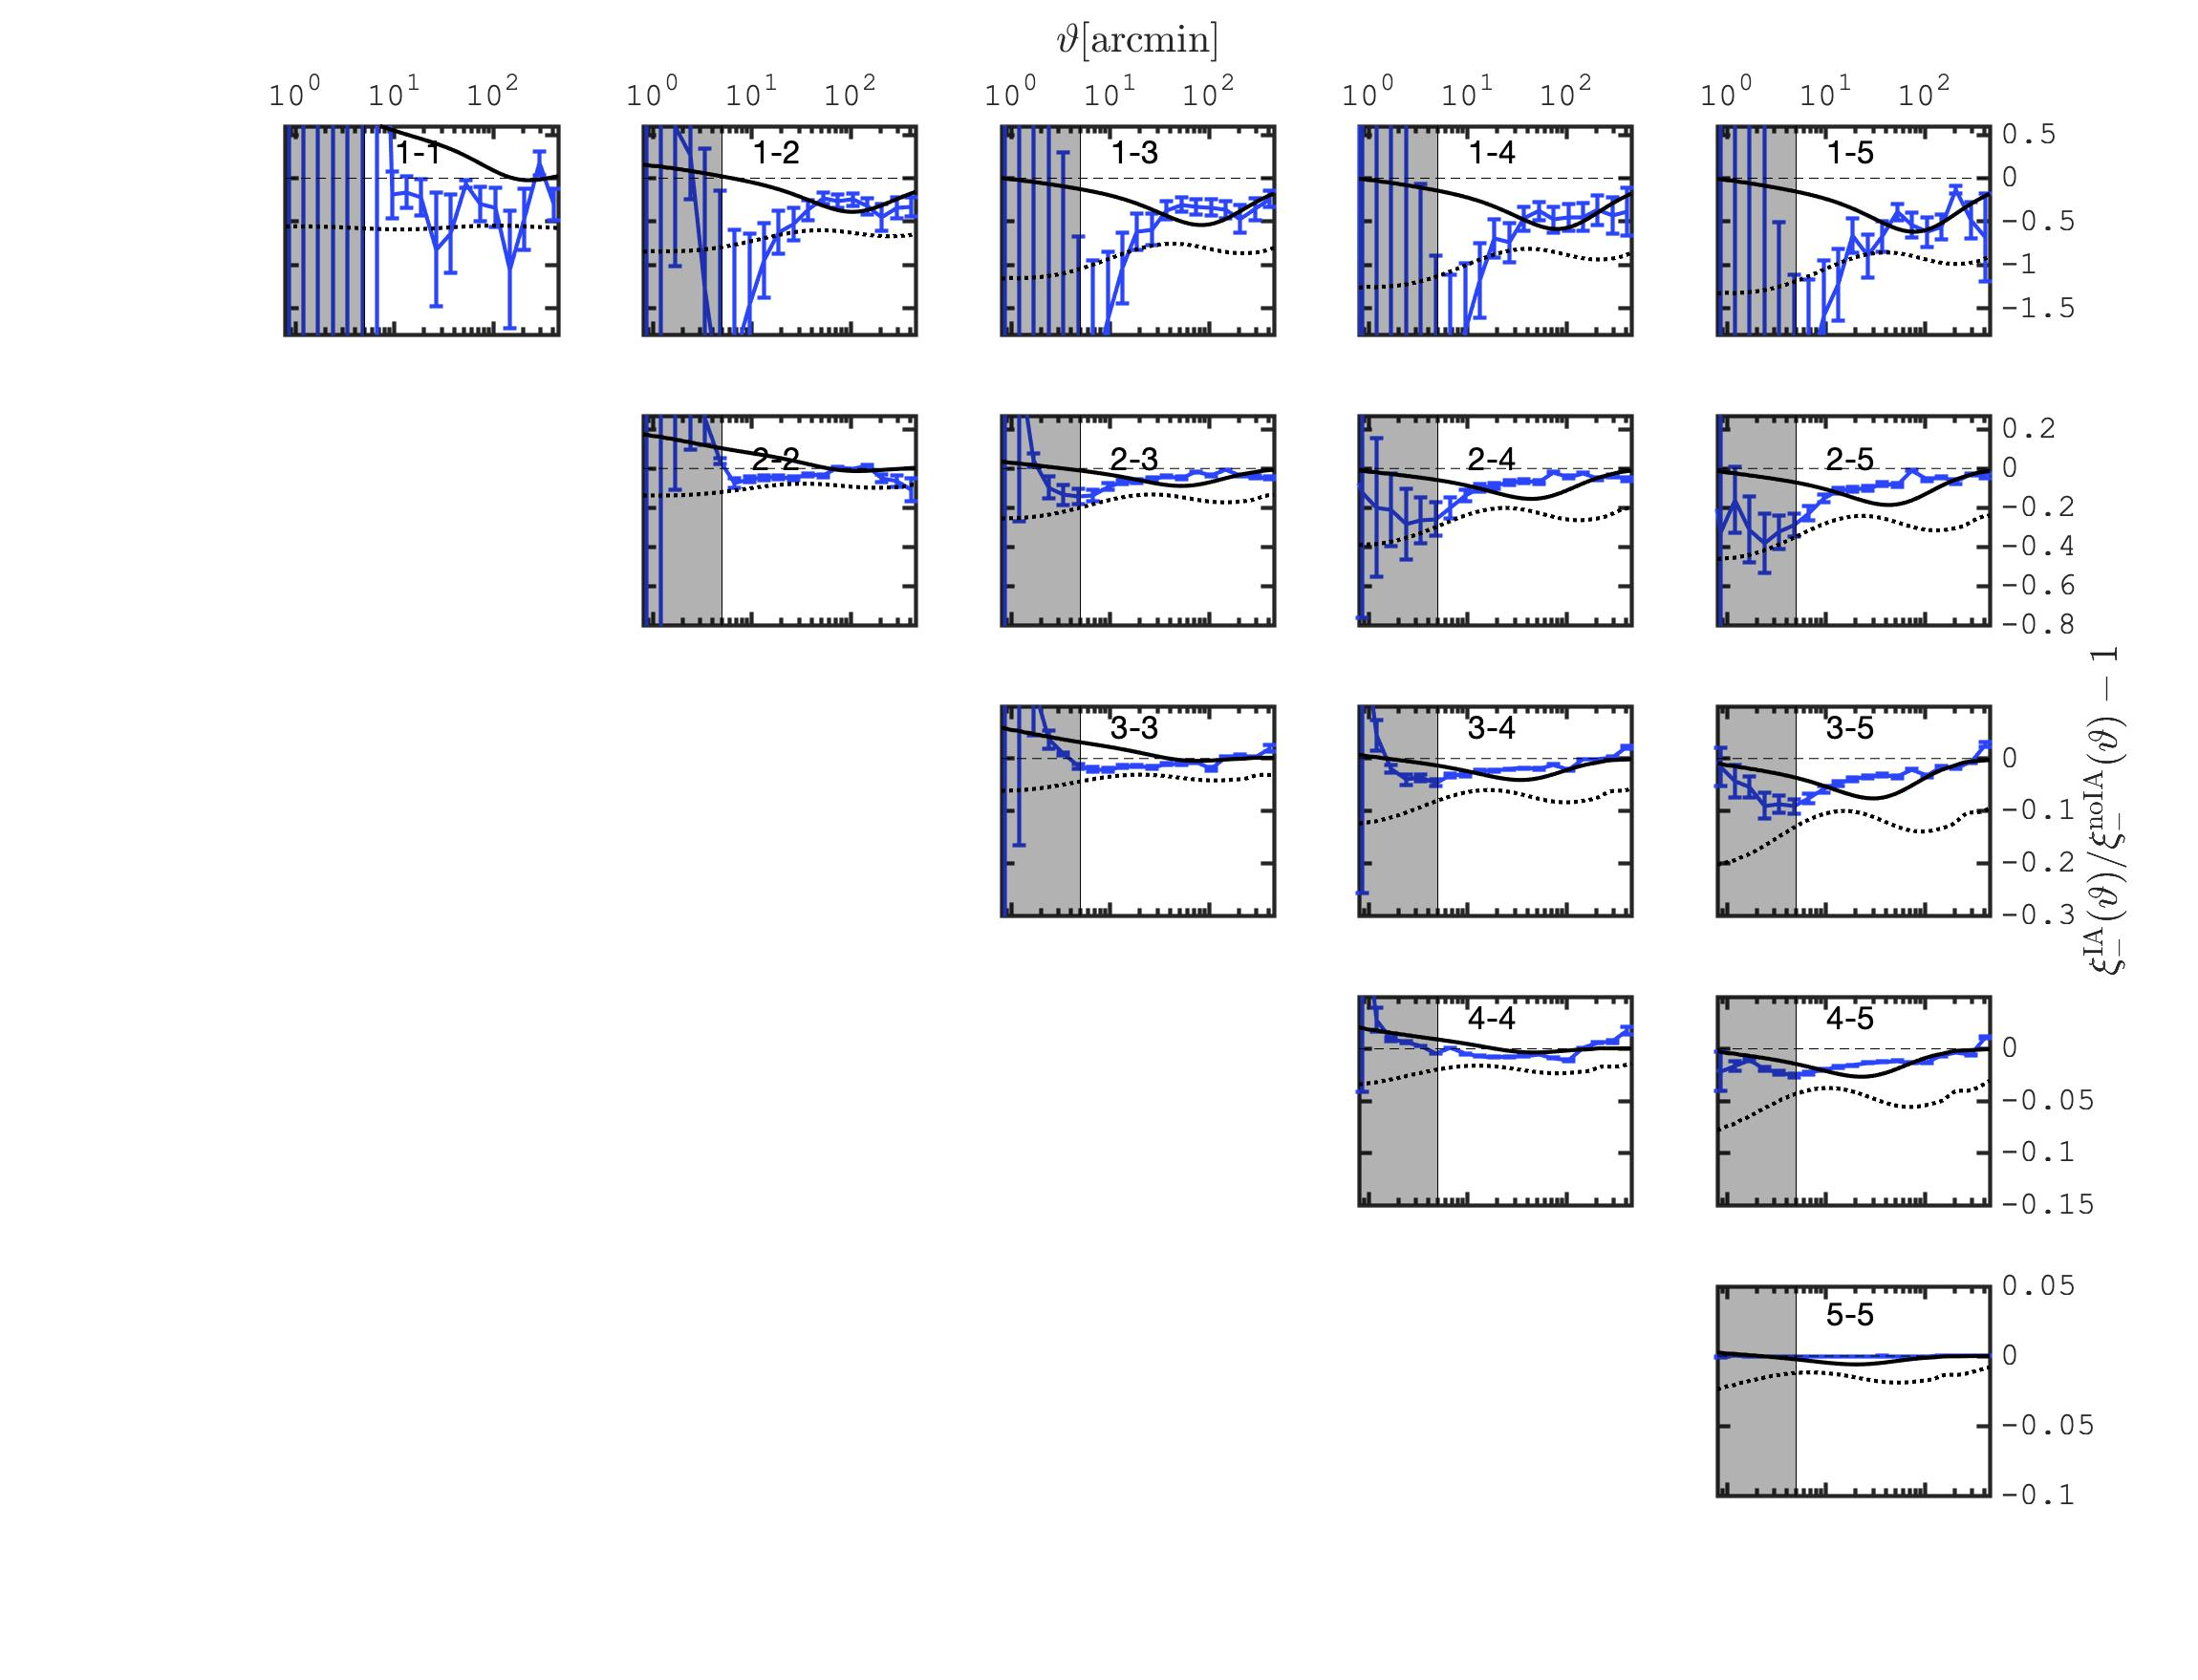
\includegraphics[width=\columnwidth]{graphs/frac_xim_sims_HOD_TT.jpg}
\caption{Same as Fig. \ref{fig:xi_deltaTT}, but showing the HOD galaxies with shapes quadratically coupled with the tidal field. }
\label{fig:xi_HOD}
\end{figure*}



The NLA and extended-NLA models respectively assume a null and a linear bias between the source galaxies and the underlying matter field, both of which are approximations to the galaxy dark matter connection. In fact, galaxies populate dark matter over-densities in a more complex manner \citep{GalaxyPopulationPapers}, which is better described by the Halo Occupation Distribution approach (HOD hereafter). The largest difference here is that these HOD galaxies are non-linear biased tracers of the matter distribution, which means that a larger number can populate regions of large over-densities, where the tidal fields are generally stronger. We therefore expect the impact of IA to be stronger in this case.

We investigate this effect with HOD galaxies extracted from the  SkySim5000 simulation \citep{SkySim5000_HOD} \footnote{We used version: {\tt skysim5000\_v1.2}, as detailed in XYZ..}, which are obtained by [...] (mention the TXPipe paper). Specifically, we select objects over a patch of 732.20 des$^2$ given by  0$<$RA$<$ 20 and -36.61$<$Dec$<$0, we apply a magnitude cut of mag$_r<$24.8, and further downsample randomly to retain 20\% of the galaxies, 
therefore matching the global galaxy redshift distribution and number density found in the rest of this paper (Eq. \ref{eq:nz}).  The sample is further split into five tomographic bins by using Charlie's magical code (Charlie), resulting in the $n(z)$ presented in Fig. \ref{fig:NzHOD}. Compared to the analytical SRD-Y1 presented in Fig. \ref{fig:Nz}, the mean redshifts of the five tomographic bins are shifted by [-0.027, -0.018,  0.003, -0.010,  0.038], respectively.

[{\it To put somewhere?: Since source clustering is a higher order effect in cosmic shear, the measured $\xi_{\pm}$ from these three mocks (random, $b_{\rm TA}=1.0$ and $b_{\rm TA}=2.0$) show negligible differences ({\it to quantify and cite}). In contrast, the impact on the IA contamination is significant and can double the secondary signal in certain circumstances. The main explanation for this is that while clustered sources are uncorrelated with the foreground matter responsible for the lensing signal, the high-density regions they live are also subject to the largest tidal fields. 
}]


\subsection{Validation with full inference}
 \label{sec:inference}
\begin{figure}
%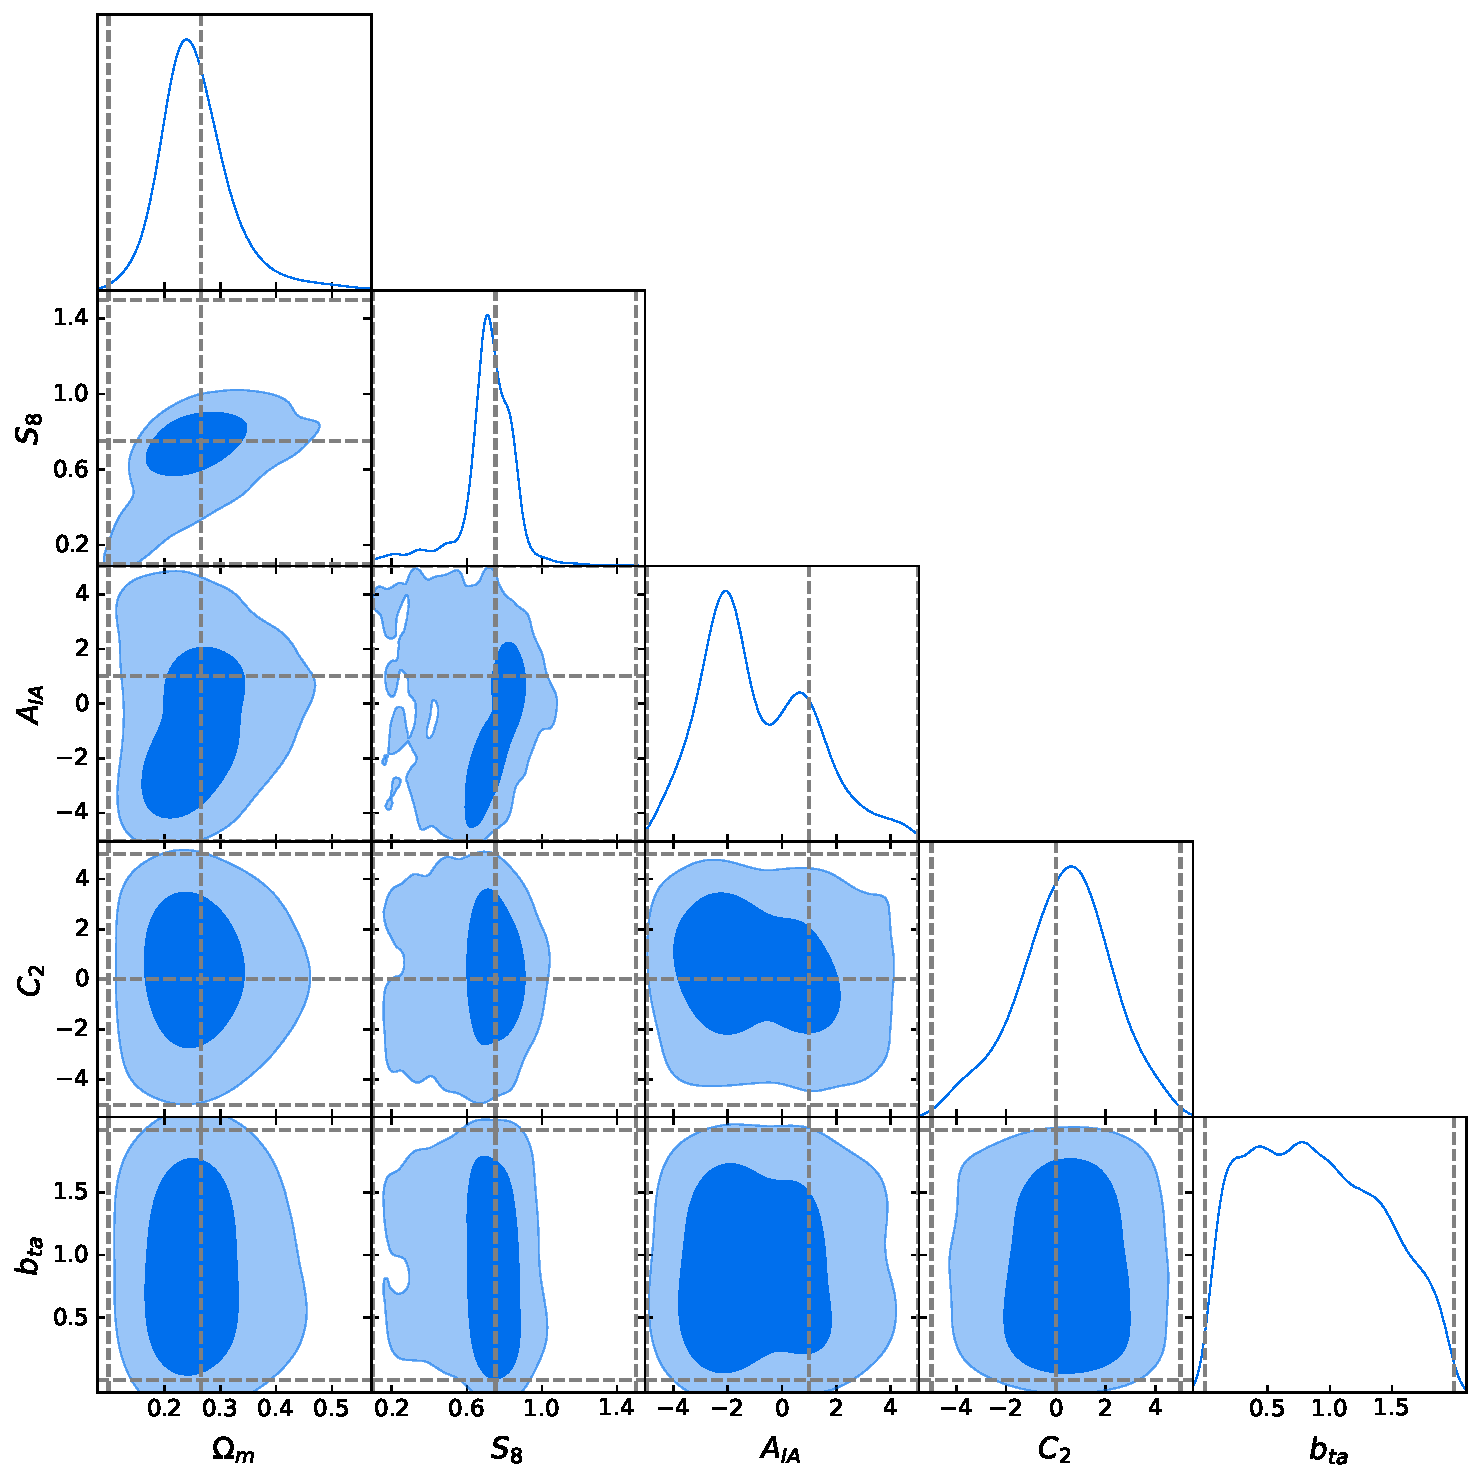
\includegraphics[width=\columnwidth]{graphs/triangle_nla_5D.pdf}
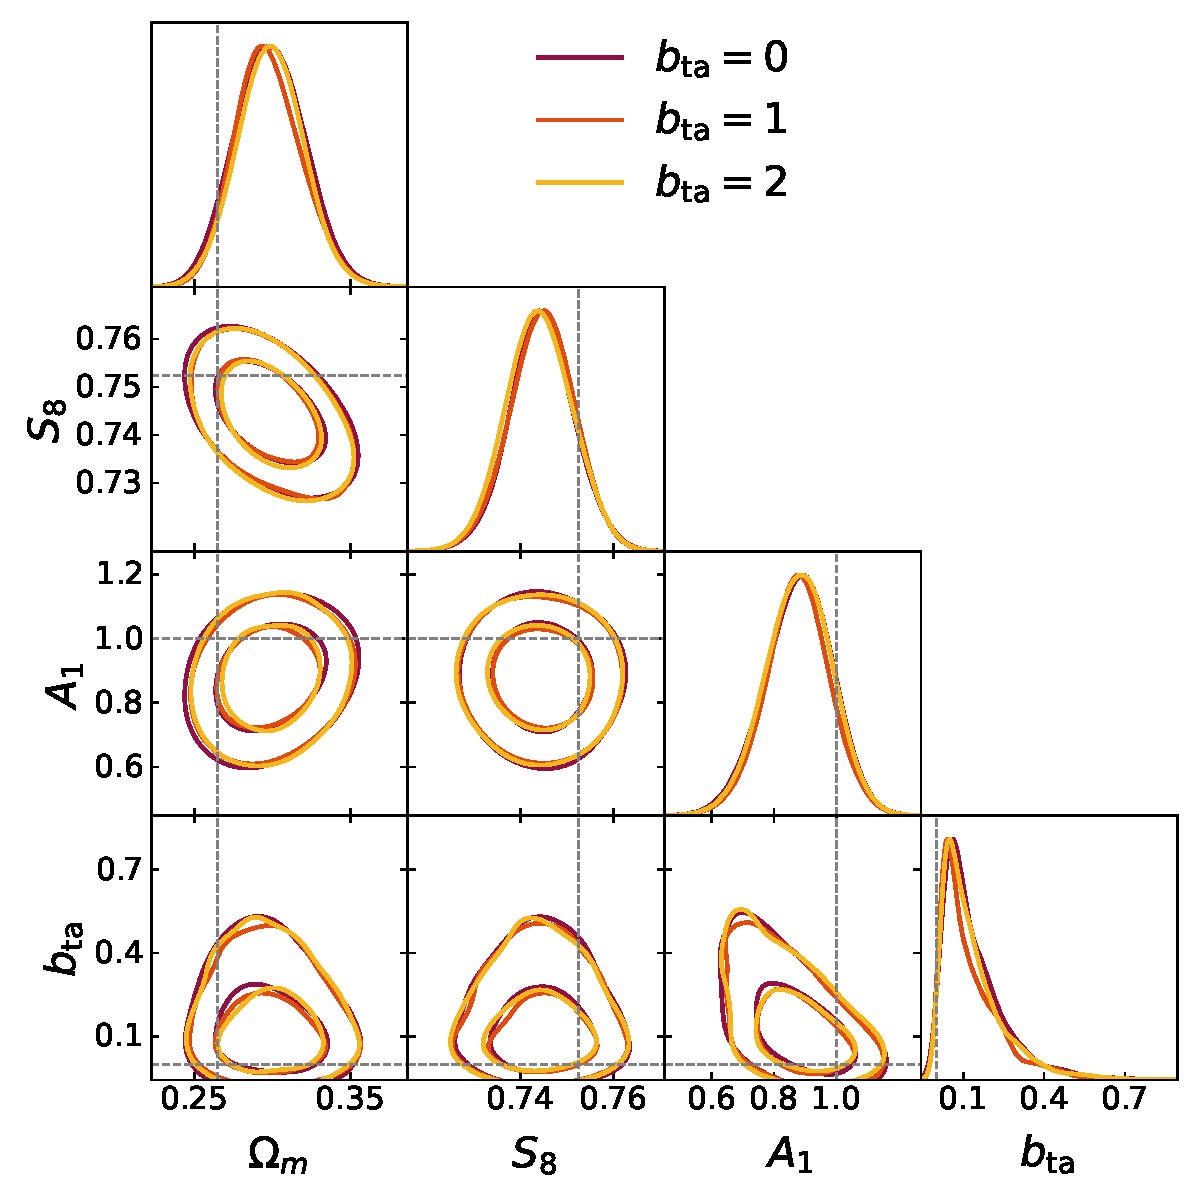
\includegraphics[width=\columnwidth]{graphs/triangle_bta_sweep.pdf}
\caption{Cosmological inference from the NLA-infused simulations, analysed the extended-NLA model. The cross-hairs represent the truth as fixed in the {\it Outer Rim} $N$-body simulations \citep{OuterRim}.}
\label{fig:triangle_nla}
\end{figure}
priors, {\sc CosmoSIS}, Takahashi $P(k)$, etc.


\section{Higher-order weak lensing statistics}
\label{sec:HOWLS}

... use the mocks from Table \ref{table:IAmodels} to compute derivatives. Show.


%----------
\section{Conclusions}
\label{sec:conclusion}
%----------

\section*{Acknowledgements}

JHD acknowledges support from an STFC Ernest Rutherford Fellowship (project reference ST/S004858/1). Ray-tracing computations were carried on the NERSC [acknowledgments] ... HACC [acknowledgements] ... {\it Outer Rim}[Acknowledgments]
\\

Some of the results in this paper have been derived using the {\sc healpy} and {\sc HEALPix} packages.
\\
\\
\\
{\footnotesize All authors contributed to the development and writing of this paper. JHD led the analysis.... }




%%%%%%%%%%%%%%%%%%%%%%%%%%%%%%%%%%%%%%%%%%%%%%%%%%
\section*{Data Availability}

 
%The SLICS numerical simulations can be found at http://slics.roe.ac.uk/, while the cosmo-SLICS can be made available upon request.
The construction of our tomographic $n^i(z)$ can be reproduced in {\tt github...CCL\_SRD\_Niko}.


%%%%%%%%%%%%%%%%%%%% REFERENCES %%%%%%%%%%%%%%%%%%

% The best way to enter references is to use BibTeX:

\bibliographystyle{hapj}
\bibliography{IA} % if your bibtex file is called example.bib


% Alternatively you could enter them by hand, like this:
% This method is tedious and prone to error if you have lots of references
%\begin{thebibliography}{99}
%\bibitem[\protect\citeauthoryear{Author}{2012}]{Author2012}
%Author A.~N., 2013, Journal of Improbable Astronomy, 1, 1
%\bibitem[\protect\citeauthoryear{Others}{2013}]{Others2013}
%Others S., 2012, Journal of Interesting Stuff, 17, 198
%\end{thebibliography}

%%%%%%%%%%%%%%%%%%%%%%%%%%%%%%%%%%%%%%%%%%%%%%%%%%

%%%%%%%%%%%%%%%%% APPENDICES %%%%%%%%%%%%%%%%%%%%%

\appendix


\begin{figure*}
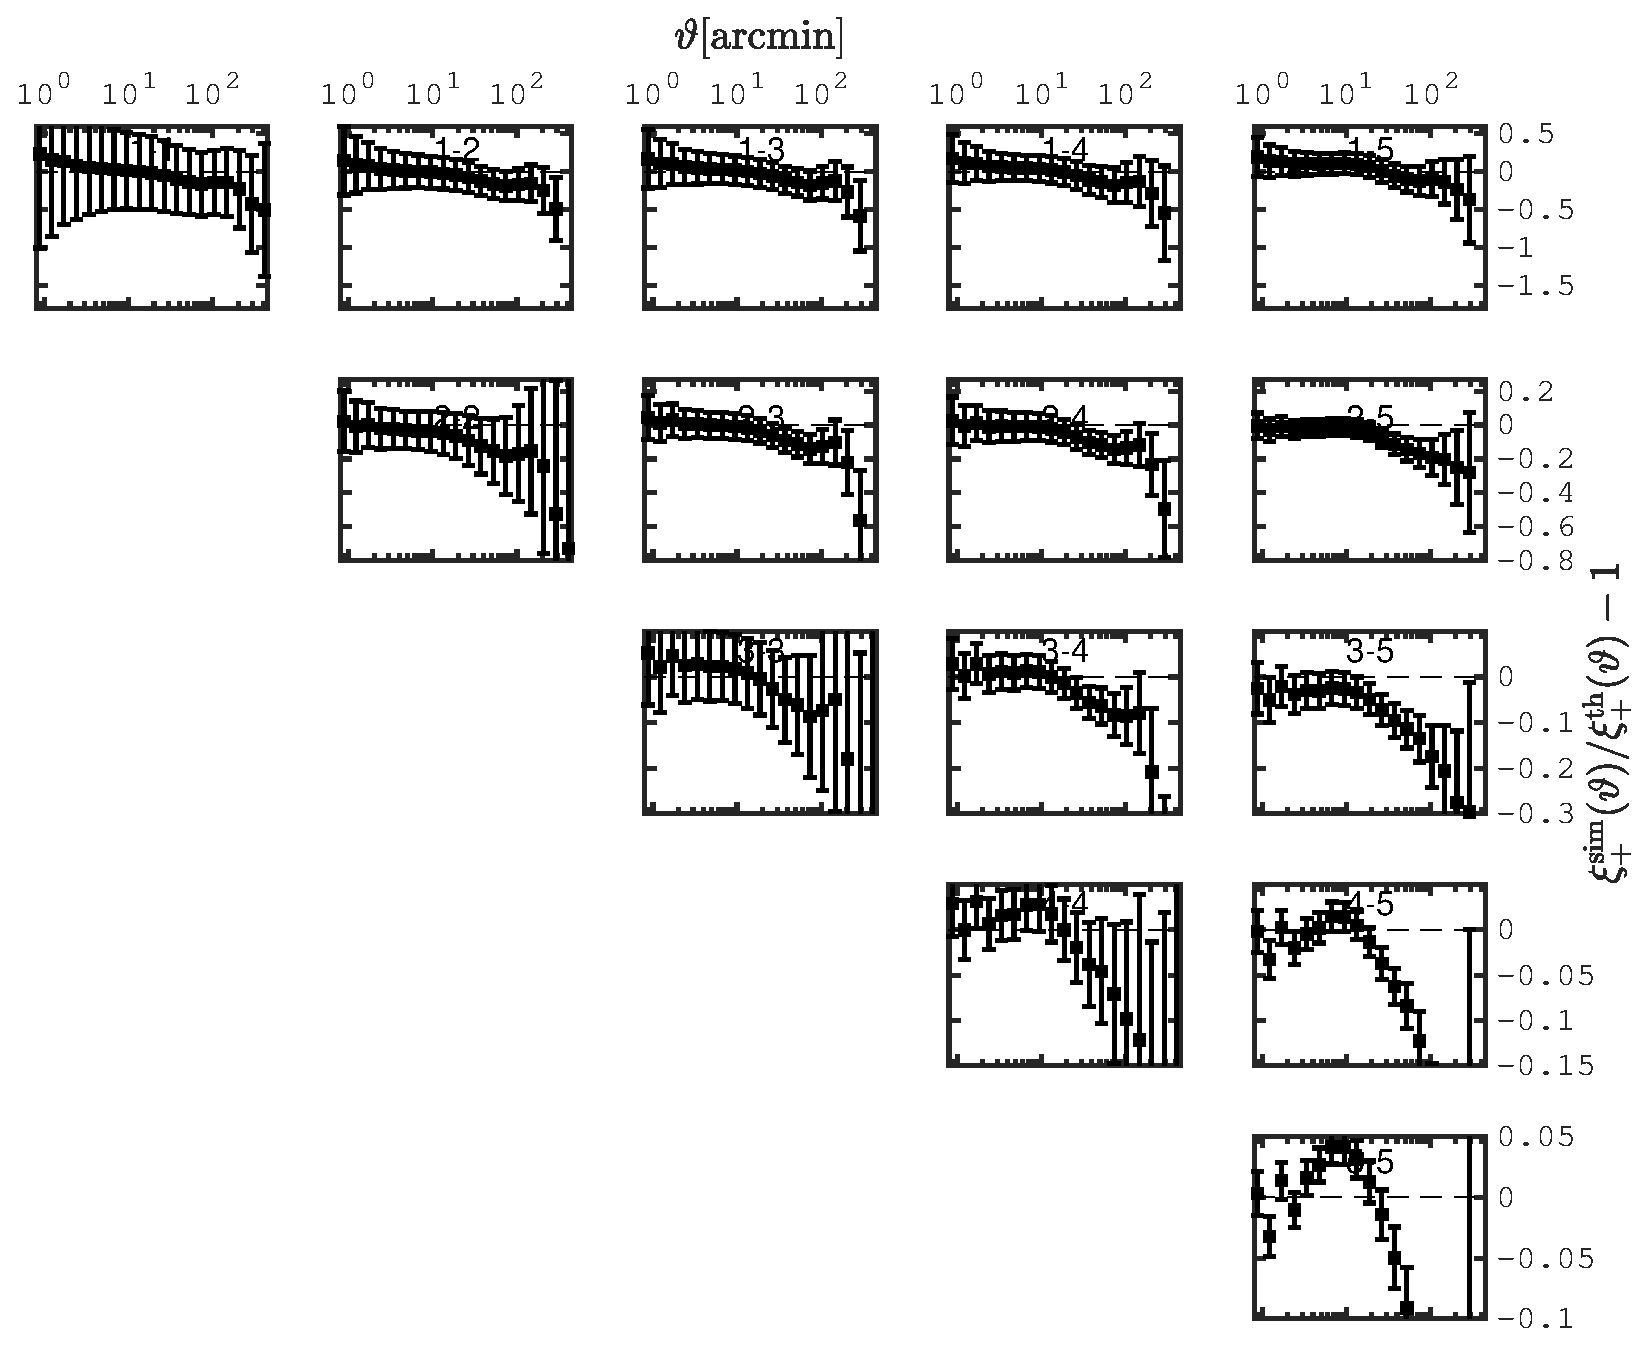
\includegraphics[width=\columnwidth]{graphs/xip_sims_vs_th.eps}
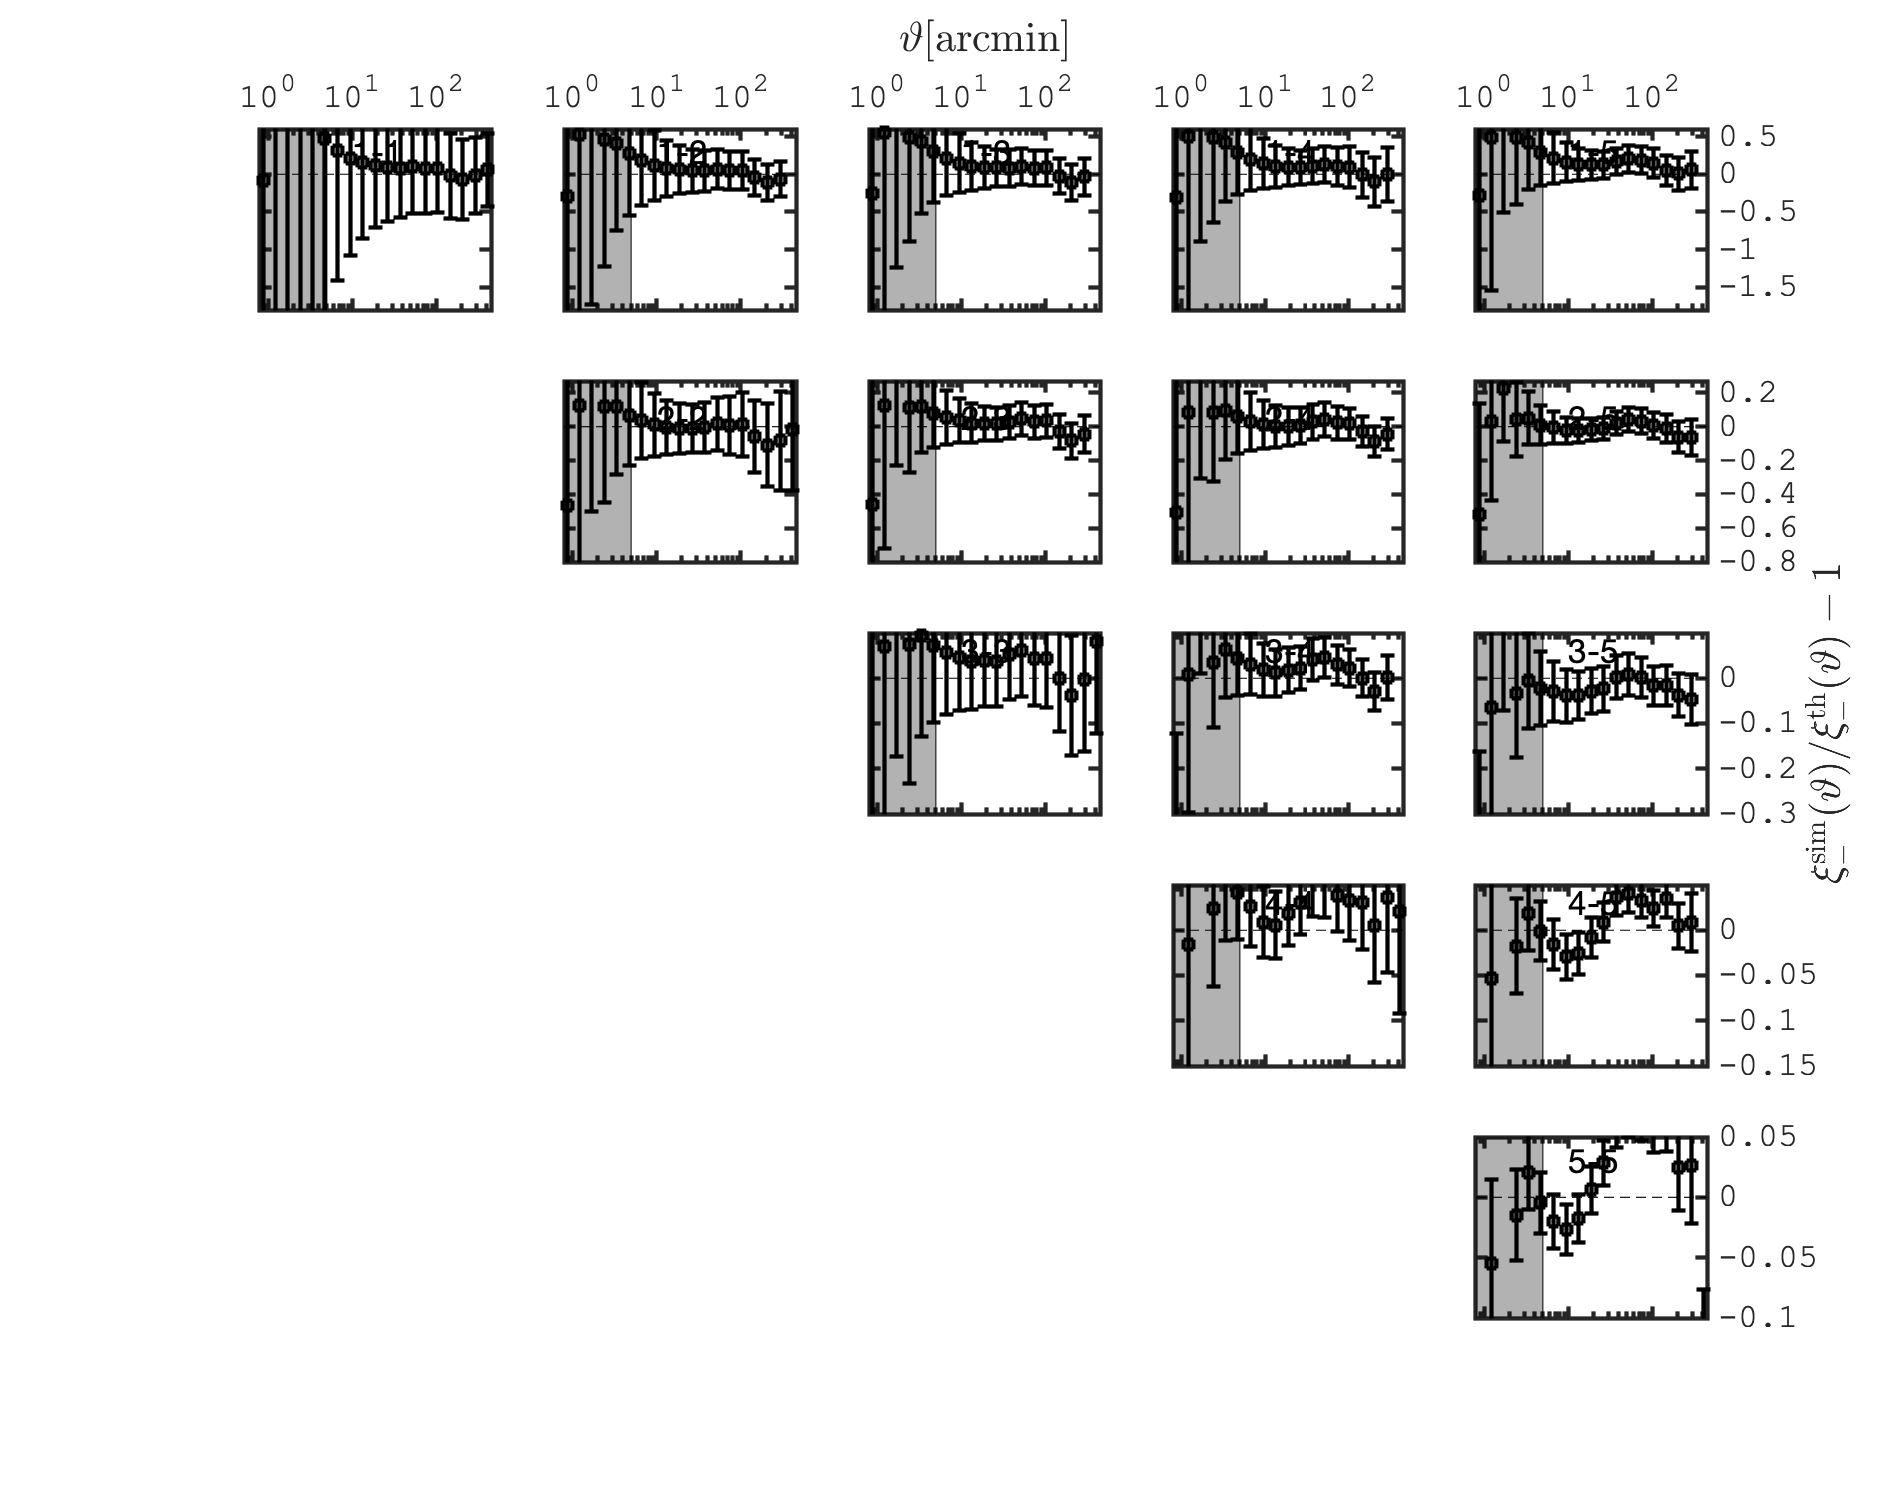
\includegraphics[width=\columnwidth]{graphs/xim_sims_vs_th.eps}
\caption{Fractional difference on $\xi_\pm$ between the measurements from SkySim5000 and the model predictions.  }
\label{fig:frac_err_sims_th}
\end{figure*}

\section{Projected Tidal Field}
\label{app:2d_TT}


\JHD{[To reword]} We derive in this Appendix...  
The prescription to assign an intrinsic alignment based on the projected tidal field, described in Eq. (\ref{eq:tidal_th}), involves the combinations $(s_{xx} - s_{yy})$ and $s_{xy}$, which therefore correspond to:
\begin{eqnarray}
 \widetilde{\epsilon}_1^{\rm IA} (\boldsymbol k_{\perp})  &\propto& \left(\frac{k_x^2 - k_y^2}{k^2} \right) \widetilde{\delta}_{\rm 2D}(\boldsymbol k_{\perp})\mathcal{G_{\rm 2D}}(\sigma_{\rm G})  \, ,\nonumber \\
 \widetilde{\epsilon}_2^{\rm IA} (\boldsymbol k_\perp)  &\propto& \left(\frac{k_x k_y}{k^2} \right) \widetilde {\delta}_{\rm 2D}(\boldsymbol k_\perp)\mathcal{G_{\rm 2D}}(\sigma_{\rm G}) 
 %\label{eq:sij}
\end{eqnarray}

Aside from the smoothing kernel, these are the same filters that are used for converting convergence maps to shear maps under the \citet[][KS hereafter]{KaiserSquires} inversion:
 \begin{eqnarray}
 \widetilde{\gamma_1} (\boldsymbol \ell)  = \left(\frac{k_x^2 - k_y^2}{k^2} \right) \widetilde {\kappa}(\boldsymbol \ell) \, , \hspace{1cm} \widetilde{\gamma_2} (\boldsymbol \ell)  = \left(\frac{k_x k_y}{k^2} \right) \widetilde {\kappa}(\boldsymbol \ell)
 %\label{eq:sij}
\end{eqnarray}
meaning that on can linearly combine the mass sheets with the correct coefficients and obtain intrinsic ellipticities from a normal KS inversion. 

Projecting out the $z$ components (e.i. $s_{0i}$=$s_{i0}$=0 for all $i$),  the tidal torque terms from Eq. (\ref{eq:tidal_th_TT}) can be expanded as:
 \begin{eqnarray}
\gamma^{\rm TT}_{ij}&=& C_2 \left[\sum_{k=x,y} s_{ik} s_{kj} -\frac{1}{3} \delta_{ij} s^2\right] \\
                                  &=&C_2 \left[ s_{ix}s_{xj}  + s_{iy}s_{yj}  -  \frac{1}{3} \delta_{ij} \left( s_{xx}^2 + s_{yy}^2 +2s_{xy}^2 \right)  \right] \, .
\end{eqnarray}
Specifically, this yields:
 \begin{eqnarray}
\gamma^{\rm TT}_{xx}&=& C_2 \left[\frac{2}{3}s_{xx}^2  -  \frac{1}{3}s_{yy}^2 + \frac{1}{3}s_{xy}^2 \right]\, ,  \nonumber \\
\gamma^{\rm TT}_{yy}&=& C_2 \left[-\frac{1}{3}s_{xx}^2  +  \frac{2}{3}s_{yy}^2 + \frac{1}{3}s_{xy}^2  \right]\, , \\
\gamma^{\rm TT}_{xy}&=& C_2 s_{xy}\left[s_{xx}+s_{yy}  \right]\, . \nonumber                                  
\end{eqnarray}
With the standard ellipticity definitions $\epsilon_1^{\rm TT}\equiv \gamma_{xx}^{\rm TT} - \gamma_{yy}^{\rm TT}$ and $\epsilon_2^{\rm TT}\equiv -2 \gamma_{xy}$, we obtain:
\begin{eqnarray}
\epsilon_1^{\rm TT} = C_2  \left[ s_{xx}^2 - s_{yy}^2\right] \, , \epsilon_2^{\rm TT} = -2 C_2 s_{xy}\left[s_{xx}+s_{yy}  \right]\, .
\end{eqnarray}
In the TATT model, the total intrinsic ellipticity component is therefore given by $\epsilon_{1/2}^{\rm IA} = \epsilon_{1/2}^{\rm TATT} = \epsilon_{1/2}^{\delta{\rm-NLA}} + \epsilon_{1/2}^{\rm TT}$.


% Don't change these lines
\bsp	% typesetting comment
\label{lastpage}
\end{document}

% End of mnras_template.tex